%%%%%%%%%%%%%%%%%%%%%%%%%%%%%%%%%%%%%%%%%%%%%%%%%%%%%%%%%%%%
%%% LIVECOMS ARTICLE TEMPLATE FOR BEST PRACTICES GUIDE
%%% ADAPTED FROM ELIFE ARTICLE TEMPLATE (8/10/2017)
%%%%%%%%%%%%%%%%%%%%%%%%%%%%%%%%%%%%%%%%%%%%%%%%%%%%%%%%%%%%
%%% PREAMBLE.
\documentclass[9pt,tutorial,pubversion]{../includes/livecoms}
% Use the 'onehalfspacing' option for 1.5 line spacing
% Use the 'doublespacing' option for 2.0 line spacing
% Use the 'lineno' option for adding line numbers.
% Use the "ASAPversion' option following article acceptance to add the DOI and relevant dates to the document footer.
% Use the 'pubversion' option for adding the citation and publication information to the document footer, when the LiveCoMS issue is finalized.
% The 'bestpractices' option for indicates that this is a best practices guide.
% Omit the bestpractices option to remove the marking as a LiveCoMS paper.
% Please note that these options may affect formatting
\usepackage{lipsum} % Required to insert dummy text
\usepackage[version=4]{mhchem}
\usepackage{siunitx}
\usepackage{listings}
\usepackage{color,soul}
\lstset{
	basicstyle=\ttfamily,
	commentstyle={},
	breakatwhitespace=true,
	breaklines=true,
	language=bash
}
\DeclareSIUnit\Molar{M}
\usepackage[italic]{mathastext}
%\graphicspath{{figures/}}
\DeclareGraphicsExtensions{.png,.eps}

%%%%%%%%%%%%%%%%%%%%%%%%%%%%%%%%%%%%%%%%%%%%%%%%%%%%%%%%%%%%
%%% IMPORTANT USER CONFIGURATION
%%%%%%%%%%%%%%%%%%%%%%%%%%%%%%%%%%%%%%%%%%%%%%%%%%%%%%%%%%%%

\newcommand{\versionnumber}{1.1}  % you should update the minor version number in preprints and major version number of submissions.
\newcommand{\githubrepository}{\url{https://github.com/biomos/gromos_tutorial_livecoms}}  %this should be the main github repository for this article

%%%%%%%%%%%%%%%%%%%%%%%%%%%%%%%%%%%%%%%%%%%%%%%%%%%%%%%%%%%%
%%% ARTICLE SETUP
%%%%%%%%%%%%%%%%%%%%%%%%%%%%%%%%%%%%%%%%%%%%%%%%%%%%%%%%%%%%
%\title{Biomolecular Simulation using the GROMOS Software Package: A set of tutorials illustrating NMR order parameter restraining and binding free-energy calculations [Article v\versionnumber]}
\title{A Suite of Advanced Tutorials for the GROMOS Biomolecular Simulation Software [Article v\versionnumber]}

\author[1]{Bettina Lier}
\author[1]{Benedict Braunsfeld}
\author[1,5]{Radek Crha}
\author[1]{Oriol Gracia Carmona}
\author[2]{Julia Gebhardt}
\author[1]{Christoph \"Ohlknecht}
\author[1,3]{Peter Poliak}
\author[1]{Peter Fraško}
\author[1]{Anita de Ruiter}
\author[2]{Marcelle B. M. Spera}
\author[1]{Michael Gillhofer}
%\author[3]{Coauthor(s) Zurich}
%\author[1,2\authfn{1}\authfn{3}]{Firstname Middlename Familyname}
%\author[2\authfn{1}\authfn{4}]{Firstname Initials Surname}
\author[4]{Wilfred F. van Gunsteren}
\author[1*,5]{Chris Oostenbrink}
\author[2*]{Niels Hansen}
\affil[1]{Institute of Molecular Modeling and Simulation, University of Natural Resources and Life Sciences, Vienna, Austria}
\affil[2]{Institute of Thermodynamics and Thermal Process Engineering, University of Stuttgart, Stuttgart, Germany}
\affil[3]{Institute of Physical Chemistry and Chemical Physics, Slovak University of Technology, Bratislava, Slovakia}
\affil[4]{Institute of Molecular Physical Science, Swiss Federal Institute of Technology, ETH, Z\"urich, Switzerland}
\affil[5]{Christian Doppler Laboratory for Molecular Informatics in the Biosciences, University of Natural Resources and Life Sciences, Vienna, Austria}
\corr{chris.oostenbrink@boku.ac.at}{CO}  % Correspondence emails.  FMS and FS are the appropriate authors initials.
\corr{niels.hansen@itt.uni-stuttgart.de}{NH}

\orcid{Bettina Lier}{0000-0002-8032-0084}
\orcid{Benedict Braunsfeld}{0000-0002-0286-8239}
\orcid{Radek Crha}{0000-0001-9293-8562}
\orcid{Oriol Gracia Carmona}{0000-0001-6560-9106}
\orcid{Julia Gebhardt}{0000-0002-5529-7337}
\orcid{Christoph \"Ohlknecht}{0000-0003-1847-1719}
\orcid{Peter Poliak}{0000-0002-6272-4907}
\orcid{Peter Fraško}{0009-0009-9491-2732}
\orcid{Anita de Ruiter}{0000-0003-3046-8969}
\orcid{Marcelle B. M. Spera}{0000-0001-7841-0489}
\orcid{Michael Gillhofer}{0000-0001-8081-6373}
\orcid{Wilfred F. van Gunsteren}{0000-0002-9583-7019}
\orcid{Chris Oostenbrink}{0000-0002-4232-2556}
\orcid{Niels Hansen}{0000-0003-4366-6120}

%\contrib[\authfn{1}]{These authors contributed equally to this work}
%\contrib[\authfn{2}]{These authors also contributed equally to this work}

%\presentadd[\authfn{3}]{Department, Institute, Country}
%\presentadd[\authfn{4}]{Department, Institute, Country}

\blurb{This LiveCoMS document is maintained online on GitHub at \githubrepository; to provide feedback, suggestions, or help improve it, please visit the GitHub repository and participate via the issue tracker.}

%%%%%%%%%%%%%%%%%%%%%%%%%%%%%%%%%%%%%%%%%%%%%%%%%%%%%%%%%%%%
%%% PUBLICATION INFORMATION
%%% Fill out these parameters when available
%%% These are used when the "pubversion" option is invoked
%%%%%%%%%%%%%%%%%%%%%%%%%%%%%%%%%%%%%%%%%%%%%%%%%%%%%%%%%%%%
\pubDOI{10.33011/livecoms.2.1.18552}
\pubvolume{2}
\pubissue{1}
\pubyear{2020}
\articlenum{18552}
\datereceived{15 September 2020}
\dateaccepted{22 December 2020}

%%%%%%%%%%%%%%%%%%%%%%%%%%%%%%%%%%%%%%%%%%%%%%%%%%%%%%%%%%%%
%%% ARTICLE START
%%%%%%%%%%%%%%%%%%%%%%%%%%%%%%%%%%%%%%%%%%%%%%%%%%%%%%%%%%%%

\begin{document}

\begin{frontmatter}
\maketitle

\begin{abstract}
This tutorial describes the practical use of some recent methodological advances implemented in the GROMOS software for biomolecular simulations. It is envisioned as a living document, with additional tutorials being added in the course of time. 
Currently, it consists of six distinct tutorials. The first tutorial describes the use of time-averaged restraints to enforce agreement with order parameters derived from NMR experiments. 
The second tutorial describes the use of extended thermodynamic integration in the double-decoupling method to compute the affinity of a small molecule to a protein. The molecule involved bears a negative charge, necessitating the application of post-simulation corrections. 
The third tutorial is based on the same molecular system, but computes the binding free energy from a path-sampling method with distance-field distance restraints and Hamiltonian replica exchange simulations. 
The fourth tutorial describes the use of Gaussian accelerated MD, an enhanced sampling technique. 
The fifth tutorial is about the use of Accelerated Enveloping Distribution Sampling (AEDS) an enhanced version of EDS. 
The sixth tutorial illustrates how to run QM/MM simulations with the Buffer Region Neural Network (BuRNN) method. 
The tutorials are written for users with some experience in the application of molecular dynamics simulations. 

%This particular document provides a skeleton illustrating key sections for a Tutorial document.
%Please see the sample \texttt{sample-document.tex} in \url{github.com/livecomsjournal/article_templates/templates} for additional information on and examples of using the LiveCoMS LaTeX class.
%Here we also assume familiarity with LaTeX and knowledge of how to include figures, tables, etc.; if you want examples, see the sample just referenced.
%
%In your work, in this particular slot, please provide an abstract of no more than 250 words.
%Your abstract should explain the main contributions of your article, and should not contain any material that is not included in the main text.
%Please note that your abstract, plus the authorship material following it, must not extend beyond the title page or modifications to the LaTeX class will likely be needed.
\end{abstract}

\end{frontmatter}

\section{Introduction}

% this is the intro
%\textcolor{red}{Here you would explain what problem you are tackling and briefly motivate your work.}
%
%\textcolor{red}{In this particular template, we have removed most of the usage examples which occur in \texttt{sample-document.tex} to provide a minimal template you can modify; however, we retain a couple of examples illustrating more unusual features of our templates/article class, such as the checklists, and information on algorithms and pseudocode.}
%
GROMOS\textsuperscript{TM} is an acronym of the GROningen MOlecular Simulation computer program package for the dynamic modelling of (bio)molecules, which has been developed since 1978 primarily as a research vehicle for methodological development \cite{wfvgn_35_years}. Written in the programming language C++, the latest version has a modular, object-oriented structure \cite{Schmid_2012}, which, together with extensive documentation \cite{volumes_1_to_9}, makes modification relatively easy. Readability of the code is prioritised over speed. The GROMOS code is freely available at \url{www.gromos.net}. The GROMOS software is to be distinguished from the GROMOS force fields for biomolecular systems. The development of the successive GROMOS force-field versions during the past 40 years has been summarised in \cite{wfvgn_35_years,Riniker_FCFF}. 
Recent work showed that time saving approximations employed during force-field development had no effect on the parametrization in terms of agreement with experiment \cite{Diem_2020, Diem_2_2020}.
The GROMOS software comes with a manual that consists of nine volumes. Volume 7 is a basic tutorial that introduces new users to the setup and analyses of molecular simulations with GROMOS \cite{volume_7}.
The set of tutorials presented here is intended to build on these original tutorials released with GROMOS.

%
\subsection{Scope}
%\textcolor{red}{Tutorials should endeavor to cover the specific task at hand, and also highlight how the steps might need to be modified (or additional care might need to be taken at particular points) to handle more general cases.}

%\textcolor{red}{The scope of the tutorial, as well as the expected proficiencies / outcomes for researchers who complete the tutorial, should be clearly defined.
%This will often happen in a specific section or subsection in the article itself.}

The four tutorials presented here cover some of the methodological advances that have been implemented in GROMOS over the last few years and are not treated in the basic tutorials distributed with the software. 
They address an advanced user who has some experience with MD simulations. Beginners in the field are recommended to start with the basic tutorial of GROMOS \cite{volume_7}. Each of the current tutorials is based on an original publication and comes with its own learning objectives and expected outcome(s). 
After completing tutorial 1 ``S2 order parameter restraining" the user should be able to
\begin{enumerate}
\item Prepare a simulation of a protein solvated in water.
\item Understand how NMR restraints are handled in GROMOS.
\end{enumerate}
%
After completing tutorial 2 ``Double decoupling method \& corrections for net-charge changes" the user should be able to
\begin{enumerate}
\item Prepare perturbation topologies for binding free energy calculations.
\item Define distance restraints and perturbed distance restraints for simulations in GROMOS.
\item Calculate binding free energies using the double decoupling method and extended-thermodynamic integration.
\item Apply a post-simulation correction scheme to correct artifacted free-energies obtained from charge-changing perturbations.
\end{enumerate}
%
After completing tutorial 3 ``Using HREMD and distance-field" the user should be able to
\begin{enumerate}
\item Setup a distance-field restraining potential-energy term.
\item Perform umbrella sampling calculations in GROMOS using perturbed distance(-field) restraints.
\item Extract the binding free energy from the potential of mean force.
\end{enumerate}
%
After completing tutorial 4 ``Selective Gaussian accelerated MD (GaMD)" the user should be able to
\begin{enumerate}
\item Prepare GaMD acceleration input files.
\item Perform GaMD parameter searches in GROMOS.
\item Perform GaMD simulations in GROMOS.
\item Extract, reweight and analyze GaMD simulations.
\end{enumerate}
%
After completing tutorial 5 ``Accelerated Enveloping Distribution Sampling (AEDS)" the user should be able to
\begin{enumerate}
\item Prepare AEDS acceleration input files.
\item Perform AEDS parameter searches in GROMOS.
\item Perform AEDS simulations in GROMOS.
\item Extract, reweight and analyze AEDS simulations as a free energy method or as a chemostat.
\end{enumerate}
%
After completing tutorial 6 “NN(QM)/MM simulations with the BuRNN approach" the user should be able to
\begin{enumerate}
\item Prepare QM input data and run QM calculations in mopac.
\item Prepare a training database and train neural networks using SchNet.
\item Run BuRNN simulations in GROMOS.
\end{enumerate}
%
Due to the statistical-mechanical nature of the ensembles of molecular configurations, meaningful values of quantities are averages over configurations or trajectories. Individual trajectories are perfectly fine for instructional purposes such as in this tutorial, but are of little utility in ``real'' research settings, unless there is little or no variation within the configurational ensemble. 
For most degrees of freedom of interest in bio-molecular systems this is certainly not the case. A simple means for generating replicates is to use different seeds of the random number generator for sampling the initial velocities at equilibration.






\section{Prerequisites}

% prerequisites
%\textcolor{red}{Here you would identify prerequisites/background knowledge that are assumed by your work, as well as any software/license requirements.}
The tutorials require the latest GROMOS11 version installed (1.5.0). 
%A GROMOS license will be issued for free upon registration of a user at \url{www.gromos.net}.  
Users can download the GROMOS source code by visiting \url{www.gromos.net} 
and registering.  Upon registration users may download the source code for free, as well as the PDF files for the manual. Files required for the basic tutorials in volume 7 of the manual can also be downloaded upon registration.
%\hl{Users who downloaded GROMOS from the website, also have access to the pdf files of the manual. 
The Program Library Manual (volume 5) \cite{volume_5} 
contains extensive documentation of the input flags. Furthermore, after compilation of the code, one can generate local documentation using doxygen.


\subsection{Background knowledge}
%\textcolor{red}{Tutorials should clearly define what concepts or abilities researchers will need to complete the tutorial (e.g., some proficiency in Python; experience with Jupyter notebooks; knowledge of classical MD; etc).}
%
%The tutorials assume the user to be familiar with the content of a GROMOS system topology, input files and analysis tools as explained in detail in the basic tutorials distributed with the software \cite{volume_7}. 
The tutorials described in this article assume the user to be familiar with the steps described in the GROMOS basic tutorial contained in volume 7 of the manual distributed with the software \cite{volume_7}. 
Specifically, users should be familiar with the content of a GROMOS system topology, input files and analysis tools explained in detail there.
Tutorial 1 (see section 3.1) repeats some of the basic system preparation steps but cannot be comprehensive in explaining all basic operations. We assume that the user is familiar with basic Linux or Unix 
command line interactions and tools to efficiently edit larger plain text files such as VIM or Emacs. Furthermore a user should be able to visualise molecular structures (e.g. with PyMOL \cite{pymol} or VMD \cite{HUMP96}) 
and to use basic plotting tools (e.g. Xmgrace, R, matplotlib).  

The GROMOS software for biomolecular simulation comprises the molecular dynamics engine MD++ and the \linebreak GROMOS++ suite of pre- and postprocessing programs. The program is independent of the computer architecture or force field used. 
The units of the various quantities are defined outside the program through a physical constants block in a force-field file. The only unit conversion performed internally by the program is between degrees and radians. The force-field files come 
in GROMOS units, that is SI units, but with atomic mass units for mass, nm for distance, ps for time, and electronic charge for charge \cite{volume_6}. No simulation protocols are prescribed. 
Input parameters specified by a user are not modified inside 
the program unless incompatible with the code. In all cases a warning message is displayed. The interpretation of the results is simplified by an extensive 
documentation of the implemented algorithms and their technical details 
in the manual available on the GROMOS web site \cite{volume_6,volume_2}.

\subsection{Software/system requirements}
%\textcolor{red}{Tutorials should clearly define what system and/or software requirements %the researcher will need to complete the tutorial (e.g., VMD version 1.9 or newer, AMBER, %etc.). Tutorials requiring specific software packages must provide instructions and files %for the referenced version of the software.}
%
GROMOS can be compiled on almost any operating system compatible with the POSIX standard.
 Some of the libraries required are not available on standard operating systems and have to be installed 
manually as described in detail in volume 8 of the GROMOS documentation \cite{volume_8}. 
In order to use the GROMOS programs without specifying the full path you can add them to your PATH variable, see section 3.2.2. in volume 8.
For some of the analyses a basic installation of Python 3 is required. 
Note that files edited on non-Unix-like operating systems may cause an I/O-error due to a different representation of a line break.




\section{Content and links}

%\textcolor{red}{This is a citiation \cite{Aivazian917}.}
%\textcolor{red}{A tutorial will normally draw on additional files and materials; clearly indicate where and how these are available, with links, and how they are being archived for the long-%term and maintained so they stay current.
%You will likely want to reference your GitHub repository as a central point to access all of this information, and then the GitHub repository may link out to other content as needed.}
The tutorials described in this article can be accessed at \githubrepository. All necessary files for completing each tutorial are provided at that location.

%\subsection{Overview}
% overview


% Tutorial 01

\subsection{Tutorial 1: $S^2$ order parameter restraining}
The backbone N-H order parameter is a measure for the spatial restriction that the N-H vector experiences in a molecular reference frame. 
Order parameters calculated from ensembles generated by MD simulations are not subject to a specific motional model but depend on the 
local flexibility inherent in the force field when solving Newton's equation of motion and on whether the assumption of internal motion 
being independent of overall tumbling is justified. 
GROMOS features a time-averaging variant of order parameter restraining that is described in detail elsewhere \cite{Hansen_S2_2014}. 
Such time-averaged restraining enhances the configurational sampling by forcing the molecule to surmount barriers that would, without restraining, only be surmounted rarely, 
that is, on longer time-scales. Moreover, a possible force-field deficiency hampering the agreement with experiment can be redressed using this restraining technique. 
In this way configurational ensembles consistent with NMR data can be generated allowing a structural interpretation of experimental observations \cite{Smith_2017,Smith_2021}.
We will demonstrate the use of time-averaged order parameters by means of the third IgG-binding domain of Protein G (GB3), which is a small 56-residue protein.

\subsubsection{Topology}
%\textcolor{green}{Should we always provide a list of input files in each subsection as well as a list of generated output files? Or should we point to vol7 for this fine structure?}
Go into the subdirectory \texttt{topo} of the directory \texttt{t\_01}. The input file \texttt{make\_top\_GB3.arg} is already prepared. We will use the force field 54a7. 
The molecular topology file for the protein, \texttt{GB3\_54a7.top}, with SPC water as a solvent can then be generated using the GROMOS++ program \texttt{make\_top} 
by typing
\begin{lstlisting}
$ make_top @f make_top_GB3.arg > GB3_54a7.top
\end{lstlisting}
In order to neutralize the net charge of -2e of the protein topology the next step is to build a topology file for a sodium ion using the input file \texttt{make\_top\_Na.arg}:
\begin{lstlisting}
$ make_top @f make_top_Na.arg > Na_54a7.top
\end{lstlisting}
Next we combine the two topologies using the GROMOS++ program \texttt{com\_top}
\begin{lstlisting}
$ com_top @f com_top_GB3_2Na.arg > GB3_2Na_54a7.top
\end{lstlisting}
The file \texttt{GB3\_2Na\_54a7.top} contains the complete molecular topology. Using the GROMOS++ program \texttt{check\_top} with the arguments \texttt{@build} and \texttt{@param} the topology can be checked against the force field. 
The 34 types of logical checks performed are listed in volume 5 of the documentation \cite{volume_5}.
Be aware that \texttt{check\_top} may not catch every inconsistency 
or that an inconsistency pointed out by \texttt{check\_top} may not necessarily indicate an error in the topology.
In the present case the putative inconsistency with the partial charge on atom 5 spotted by \texttt{check\_top} is 
actually not an error because the partial charge is adapted for the N-terminus of the peptide chain.
Therefore, it is important to assure oneself that the topology generated is the one intended.

\subsubsection{Coordinates}

Go into the subdirectory \texttt{coord}. The Cartesian coordinates for the protein can be downloaded from the Protein Databank, accession code 2OED \cite{Ulmer_2003}. By using the GROMOS++ program \texttt{pdb2g96} the PDB file will be converted to a GROMOS coordinate file. Before conversion we make a copy of the downloaded pdb file \texttt{2oed.pdb} into the file \texttt{2oed\_edited.pdb}. In the latter we do a change in line 1010 (replace “O~” by “O1”) and line 1016 (replace “OXT” by “O2~”) such that \texttt{pdb2g96} recognizes these two atoms as belonging to the carboxy terminus. When editing the PDB file the columns must be kept aligned. The remaining differences between the nomenclature used in the PDB file and the one used in the topology are handled via the file \texttt{pdb2g96.lib}. With
\begin{lstlisting}
$ pdb2g96 @f pdb2g96_GB3.arg > pdb2g96_GB3.cnf
\end{lstlisting}
we generate a GROMOS coordinate file. 
Since the used NMR structure contains more hydrogen atoms than needed by the united-atom GROMOS force field, merging aliphatic hydrogen and carbon atoms into one interaction site, 
a list of warnings regarding ignored hydrogen atoms is issued, which can be ignored. If the initial structure was determined using X-ray diffraction, missing hydrogen atoms can be generated 
with the GROMOS program \texttt{gch} as explained in the basic tutorial.

\subsubsection{Energy minimization}

Before putting the protein in a box of solvent, its configuration is relaxed by energy minimization 
in vacuo to release possible strain induced by small differences in bond lengths, bond angles, improper dihedral angles and short non-bonded contacts 
between the force-field parameters and the NMR structure.
Go into the subdirectory \texttt{min} and open the shell script \texttt{em\_GB3.run} to adapt the paths and the names of the files according to your system. 
The energy minimization of the solute in vacuo is very fast and can be run interactively by typing
\begin{lstlisting}
$ ./em_GB3.run
\end{lstlisting}
Once the energy minimization is finished the minimized coordinates are written to the file \texttt{GB3\_min.cnf} and the general output file \texttt{em\_GB3.omd} contains the progress of the minimization.

\subsubsection{Solvating the protein in a water box}

Now the protein is ready to be placed into a box and solvated for subsequent simulations under periodic boundary conditions. Go into the subdirectory \texttt{box}. The box shape will be chosen to be rectangular, the simple point charge (SPC) water model \cite{Berendsen1981} will be employed (as already specified in the topology file), the minimum solute-to-wall distance will be 1.2 nm such that the closest surface atoms of two periodic copies are at least 2.4 nm apart (longer than the cutoff distance of 1.4 nm). The minimum solute-solvent distance is set to 0.23 nm. The GROMOS++ program \texttt{sim\_box} is used to generate the box and to solvate the protein by executing
\begin{lstlisting}
$ sim_box @f sim_box_GB3.arg > sim_box_GB3.cnf
\end{lstlisting}
During the immersion into the solvent, water molecules may still have been placed too close or too far away relative to the protein surface. Moreover, their orientation towards the protein surface is not optimized. Therefore, we need an equilibration of the solute-solvent system using energy minimization. During this process the solute atoms will be positionally restrained around their coordinates in the initial structure using harmonic springs while the solvent molecules can move freely. The list of atoms to be positionally restrained must be specified in a file \texttt{sim\_box\_GB3.por}. The reference positions of these atoms must be specified in a separate file \texttt{sim\_box\_GB3.rpr}. To prepare these files, copy the coordinate file \texttt{sim\_box\_GB3.cnf} to \texttt{sim\_box\_GB3.por} and \texttt{sim\_box\_GB3.rpr}. Open the file \texttt{sim\_box\_GB3.por} in your text editor and
\begin{itemize}
\item	Write in the title block the text “list of solute atoms to be positionally restrained”
\item	Change the keyword “POSITION” at the beginning of the atom coordinate block into the keyword “POSRESSPEC”
\item	Delete all the solvent atoms. This can also be conveniently achieved by using the command line instruction \lstinline !$ sed -i "/SOLV/d"! \lstinline! sim_box_GB3.por!
\end{itemize}
When GROMOS reads this file, it will entirely ignore the coordinates and just look at the list of atoms. Next, open the \texttt{sim\_box\_GB3.rpr} in your text editor and
\begin{itemize} 
\item	Write in the title block the text “reference positions of solute atoms to be positionally restrained”
\item	Change the keyword “POSITION” at the beginning of the atom coordinate block into the keyword “REFPOSITION”
\end{itemize}
When GROMOS reads this file, it will only use the coordinates of the atoms listed in \texttt{sim\_box\_GB3.por} and ignore the rest. 
Now, adapt the input file \texttt{em\_solvent.imd} according to the number of solvent molecules in your box by adjusting the second number in the \texttt{SYSTEM} block and by adjusting the index of the last atom in the \texttt{FORCE} block.
Now, adapt the paths and the names of the files in \texttt{em\_solvent.run} according to your system. 
Then start the energy minimization of the solvent interactively by typing 
\begin{lstlisting}
$ ./em_solvent.run
\end{lstlisting}
This will take a few moments. Once the minimization is finished, the new coordinate file, \texttt{GB3\_h2o.cnf} and the general output file \texttt{em\_solvent.omd} will be written out. 

\subsubsection{Adding counter ions}

To complete the preparation of the simulation box two sodium ions should be added. Go to the subdirectory \texttt{ion}. The two sodium ions are added to the simulation box using the GROMOS++ program \texttt{ion} such that they replace the water molecules which have the lowest electrostatic potential. You can run \texttt{ion} by typing
\begin{lstlisting}
$ ion @f ion_GB3.arg > GB3_2Na_h2o.cnf
\end{lstlisting}

\subsubsection{Thermalisation and equilibration}
For thermalisation we will use a combination of a progressively increasing temperature and progressively decreasing position restraints on the solute atoms. The thermalisation procedure is facilitated by the use of the GROMOS++ program \texttt{mk\_script}, which allows the automatic generation of successive MD jobs that (i) slightly differ in their input parameters; (ii) use the final configuration and velocities of one job as the starting configuration and velocities of the next one; (iii) automatically submit the next job upon completion of the previous one. Go into the subdirectory \texttt{eq}. Before running the script you need to adjust the number of solvent molecules and the last atom for the set of degrees of freedom in the input file \texttt{equilibration.imd} as well as the paths and names in \texttt{eq\_mk\_script.arg}. Moreover new position restraint files \texttt{GB3\_2Na\_h2o.por} and \texttt{GB3\_2Na\_h2o.rpr} have to be prepared as described above based on the output file \texttt{GB3\_2Na\_h2o.cnf} from the \texttt{ion} program. Now the job scripts and corresponding input files are created by typing
\begin{lstlisting}
$ mk_script @f eq_mk_script.arg
\end{lstlisting}
You are now ready to start the thermalisation and equilibration. Run the first job script and the others will be automatically executed as soon as the preceding script has finished.
\begin{lstlisting}
./eq_GB3_1.run
\end{lstlisting}
After the equilibration is finished you can carry out some basic checks in the \texttt{eq/ana} directory. You can for example see that the kinetic energy is increasing at every new job.

\subsubsection{Unrestrained molecular dynamics simulation}
The equilibration procedure produced short simulations at constant temperature and volume. Now we want to elongate the simulation to 21 ns under constant temperature and pressure. Go to the directory \texttt{md} and use the \texttt{mk\_script} program to create the job scripts and input files:
\begin{lstlisting}
$ mk_script @f md_mk_script.arg
\end{lstlisting}
Here the simulation is split into 21 jobs that may preferably run on a computer cluster. To run the jobs interactively type
\begin{lstlisting}
$ ./md_GB3_1.run
\end{lstlisting}
To facilitate the submission to a cluster, adjust the entry \texttt{lastcommand} in the file \texttt{mk\_script.lib}. Depending on your cluster settings, you may also want adjust the entry \texttt{workdir} and 
make sure to use a binary that runs GROMOS in parallel (MPI or openMP) or uses the GPU acceleration \cite{volume_8}.

\subsubsection{$S^2$-order parameter restrained molecular dynamics simulation}

Starting again from the final configuration of the equilibration procedure we now perform the $S^2$ order parameter restraining simulation. Go to the directory \texttt{md\_S2res} and have a look into the input file \texttt{md.imd}. 
Compared to the unrestrained simulation it contains the additional block 

\begin{lstlisting}
ORDERPARAMRES
# NTOPR NTOPRA COPR TAUOPR UPDOPR NTWOP
   -1    0    300     200   1     250
END
\end{lstlisting}
By setting the switch \texttt{NTOPR} to \texttt{-1} you specifiy that you use time-averaged restraining without individual weights for the force constant. The switch \texttt{NTOPRA} controls reading of the 
averages from the startup file. The value should be \texttt{0} for the first job and \texttt{1} for continuation jobs. The switch \texttt{COPR} defines the order parameter restraining force constant. With 
\texttt{TAUOPR} the coupling time is specified. The switch \texttt{UPDOPR} is only relevant if the averages are not calculated using the damped memory approach but as a running average covering the 
last \texttt{TAUOPR} picoseconds of the simulation. We note that window averaging shows no advantage over the damped memory approach while requiring a sizeable amount of RAM. Finally \texttt{NTWOP}
controls how often the order parameters are written to the special trajectory. 
The actual settings of the switches \texttt{NTOPRA}, \texttt{COPR} and \texttt{TAUOPR} are defined in the joblist \texttt{S2\_restraining.jobs} that has the following structure: 
\begin{lstlisting}
TITLE
S2 order parameter restraining
END
JOBSCRIPTS
job_id [...] NTOPR NTOPRA COPR TAUOPR [...]
   1   [...]    -1   0     10    200  [...]   
   2   [...]    -1   1    300    200  [...] 
   3   [...]    -1   1    300    200  [...] 
... 
END
\end{lstlisting}
In the first job we start with a small restraining force constant \texttt{COPR} since we want a gentle build-up of the time averages. From the second job onwards the force constant is unchanged. Similar settings of force constant and averaging time were used in previous work on this system \cite{Hansen_S2_2014}.
The experimental order parameters used for the restraining are taken from Hall and Fushmann \cite{Hall_2003} and are specified in the column \texttt{S0} of the file \texttt{order\_exp.dat}.
In the latter file the atoms \texttt{i} and \texttt{j} defining the bond vector need to be specified as well as the average bond length \texttt{R0}. 
In the column \texttt{DSO} the flat-bottom parameter of the restraining potential-energy term is set to 0.05. Therefore, no restraining force is applied if the absolute value of the difference between simulation and experiment is smaller than or equal to this value.
%The column \texttt{DS0} contains the width of the flat bottom region while
With \texttt{WOPR} individual weights can be assigned to the order parameters if the corresponding switch \texttt{NTOPR} in \texttt{md.imd}
is selected. Now use the \texttt{mk\_script} program to create the job scripts and input files:
\begin{lstlisting}
$ mk_script @f md_mk_script.arg
\end{lstlisting}
The file \texttt{order\_exp.dat} needs to be specified under the keyword \texttt{order} in the \texttt{@files} section of \texttt{md\_mk\_script.arg}.
As before the simulation is split into 21 jobs that may preferably run on a computer cluster. To run the jobs interactively type
\begin{lstlisting}
$ ./md_GB3_1.run
\end{lstlisting}

\subsubsection{Analysis}
First, we analyse the energy trajectories of the unrestrained and restrained simulations. Go into the directory \texttt{ana/ene\_ana/unres} and run the analysis program \texttt{ene\_ana} by typing
\begin{lstlisting}
$ ene_ana @f ene_ana_unres.arg > ene_ana_unres.out
\end{lstlisting}
The first trajectory is excluded from the analysis to account for the fact that the system needs some additional equilibration phase when switching from a constant volume to a constant pressure simulation.
The file \texttt{ene\_ana\_unres.out} contains the averages while the time series of all specified properties are contained in the \texttt{.dat} files. The total intramolecular energy of the protein 
had to be defined in the \texttt{ene\_ana.md++.lib} file located in the subdirectory above, see line 150 in that file. Repeat the analysis for the restrained simulation and compare the results. For the latter we additionally 
evaluate the total restraining energy in order to check whether the contribution of the restraints is small compared to the total intramolecular energy of the protein. 
Note that the file \texttt{ene\_ana.md++.lib} has to be compatible with the GROMOS version used. If you use a newer version than 1.5.0, you will find the corresponding file in the directory \texttt{md++-x.y.z/data}.

Second, the atom positional root-mean-square deviation of the backbone atoms from a reference structure is calculated for the two trajectories using the GROMOS++ program \texttt{rmsd}. 
For the unrestrained simulation go to the directory \texttt{ana/rmsd/unres} and type
\begin{lstlisting}
$ rmsd @f rmsd_unres.arg > rmsd_unres.out
\end{lstlisting}
Here, we use the last structure of the equilibration simulation as reference. The two resulting RMSD time series are shown in Figure~\ref{GB3_rmsd}. 

Third, the root-mean-square fluctuation of the backbone N atoms is calculated using the program \texttt{rmsf}. For the unrestrained simulation go to the directory \texttt{ana/rmsf/unres} and type
\begin{lstlisting}
$ rmsf @f rmsf_unres.arg > rmsf_unres.out
\end{lstlisting}
The two resulting plots are displayed in Figure~\ref{GB3_rmsf} and show that the restrained simulation does not necessarily show less fluctuations compared to the unrestrained simulation.
% although the order parameters are mostly larger. 

Finally the N-H order parameters are calculated using the program \texttt{nhoparam}. For the unrestrained simulation go to the directory \texttt{ana/nhoparam/unres/0.5} and type
\begin{lstlisting}
$ nhoparam @f nhoparam_unres.arg > nhoparam_unres.out
\end{lstlisting}
We do the analysis using two averaging time windows of 0.5 and 1.0 ns, respectively. Since the order parameter is defined as long-time tail of the autocorrelation function of the bond vector, this comparison provides 
insight whether the corresponding autocorrelation functions have reached their plateau values. The \texttt{nhoparam} program also calculates order parameters averaged over the entire trajectory. These values 
may be considerably smaller than those calculated using 1 ns averaging time. If that is the case, conformational changes occur on larger time scales and a structural interpretation based on order parameters might be difficult.
Figure~\ref{GB3_S2} shows a relatively small influence of the averaging time on the resulting order parameters in the present case. 

\begin{figure}[H]
\centering
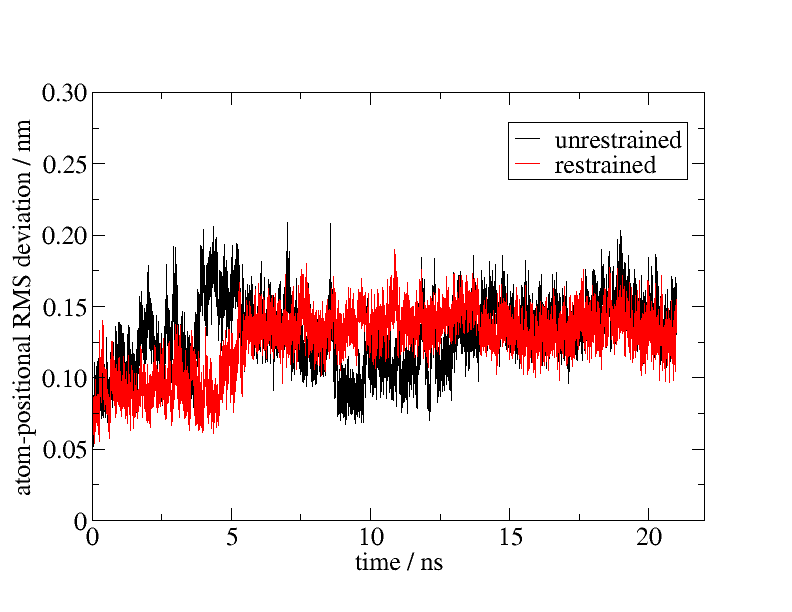
\includegraphics[scale=.3]{../04_tutorial_01/figures/GB3_RMSD}
\caption{Backbone atom-positional root-mean-square deviation (RMSD) of GB3 with respect to the final structure of the equilibration simulation.}
\label{GB3_rmsd}
\end{figure}

\begin{figure}[H]
\centering
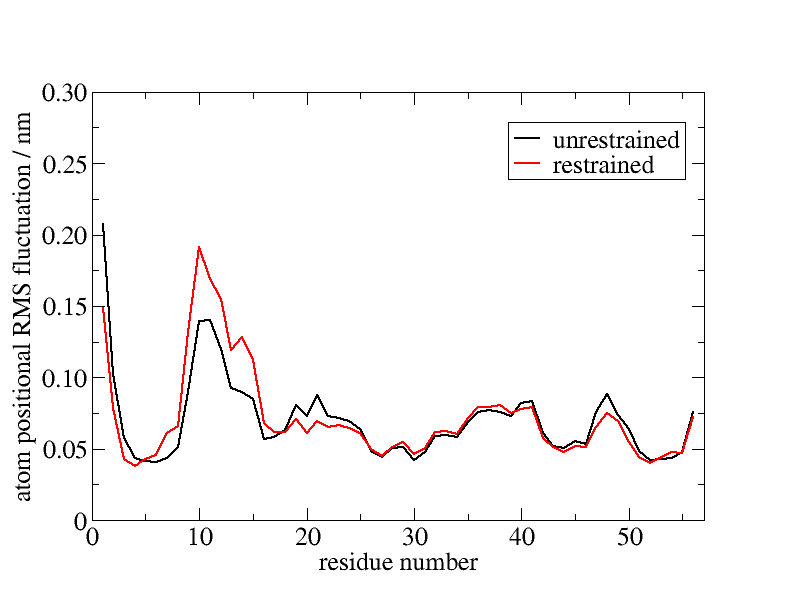
\includegraphics[scale=.3]{../04_tutorial_01/figures/GB3_RMSF}
\caption{Backbone N atom-positional root-mean-square fluctuation (RMSF) of GB3.}
\label{GB3_rmsf}
\end{figure}

\begin{figure}[H]
\centering
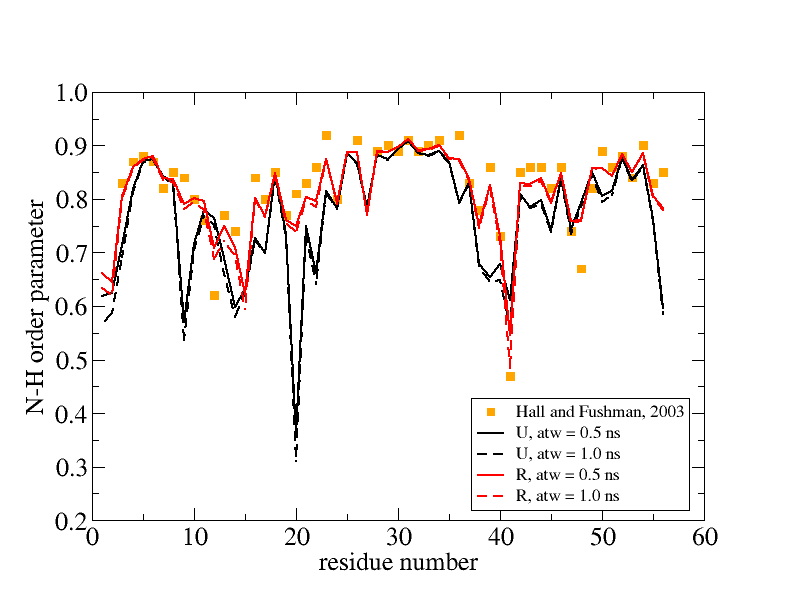
\includegraphics[scale=.3]{../04_tutorial_01/figures/GB3_S2}
\caption{Comparison of backbone N-H order parameters for protein GB3, determined from unrestrained (U) and restrained (R) MD simulations using different averaging time windows (atw) in the analysis. The experimentally derived order parameters used for restraining were taken from the work of Hall and Fushman ~\cite{Hall_2003} (anisotropic model).}
\label{GB3_S2}
\end{figure}










% Tutorial 02

\subsection{Tutorial 2: Double decoupling method \& corrections for net-charge changes} \label{chap:tut2}
The double decoupling method (DDM)~\cite{DDM} is an alchemical perturbation approach to compute binding free energies from molecular dynamics simulations by making use of a thermodynamic cycle (Figure \ref{TC_ASA}). Two of the branches are determined by thermodynamic integration corresponding to the decoupling of the ligand from the system (perturbing the ligand into a non-interacting dummy molecule), free in solution and when bound to the host. In order to avoid sampling of non-relevant phase space in the complexed system, the ligand is kept in a position that resembles that of the native bound conformation by gradually introducing a harmonic distance restraint. The free energy of the restraint removal can be evaluated analytically.

\begin{figure}[H]
    \centering
    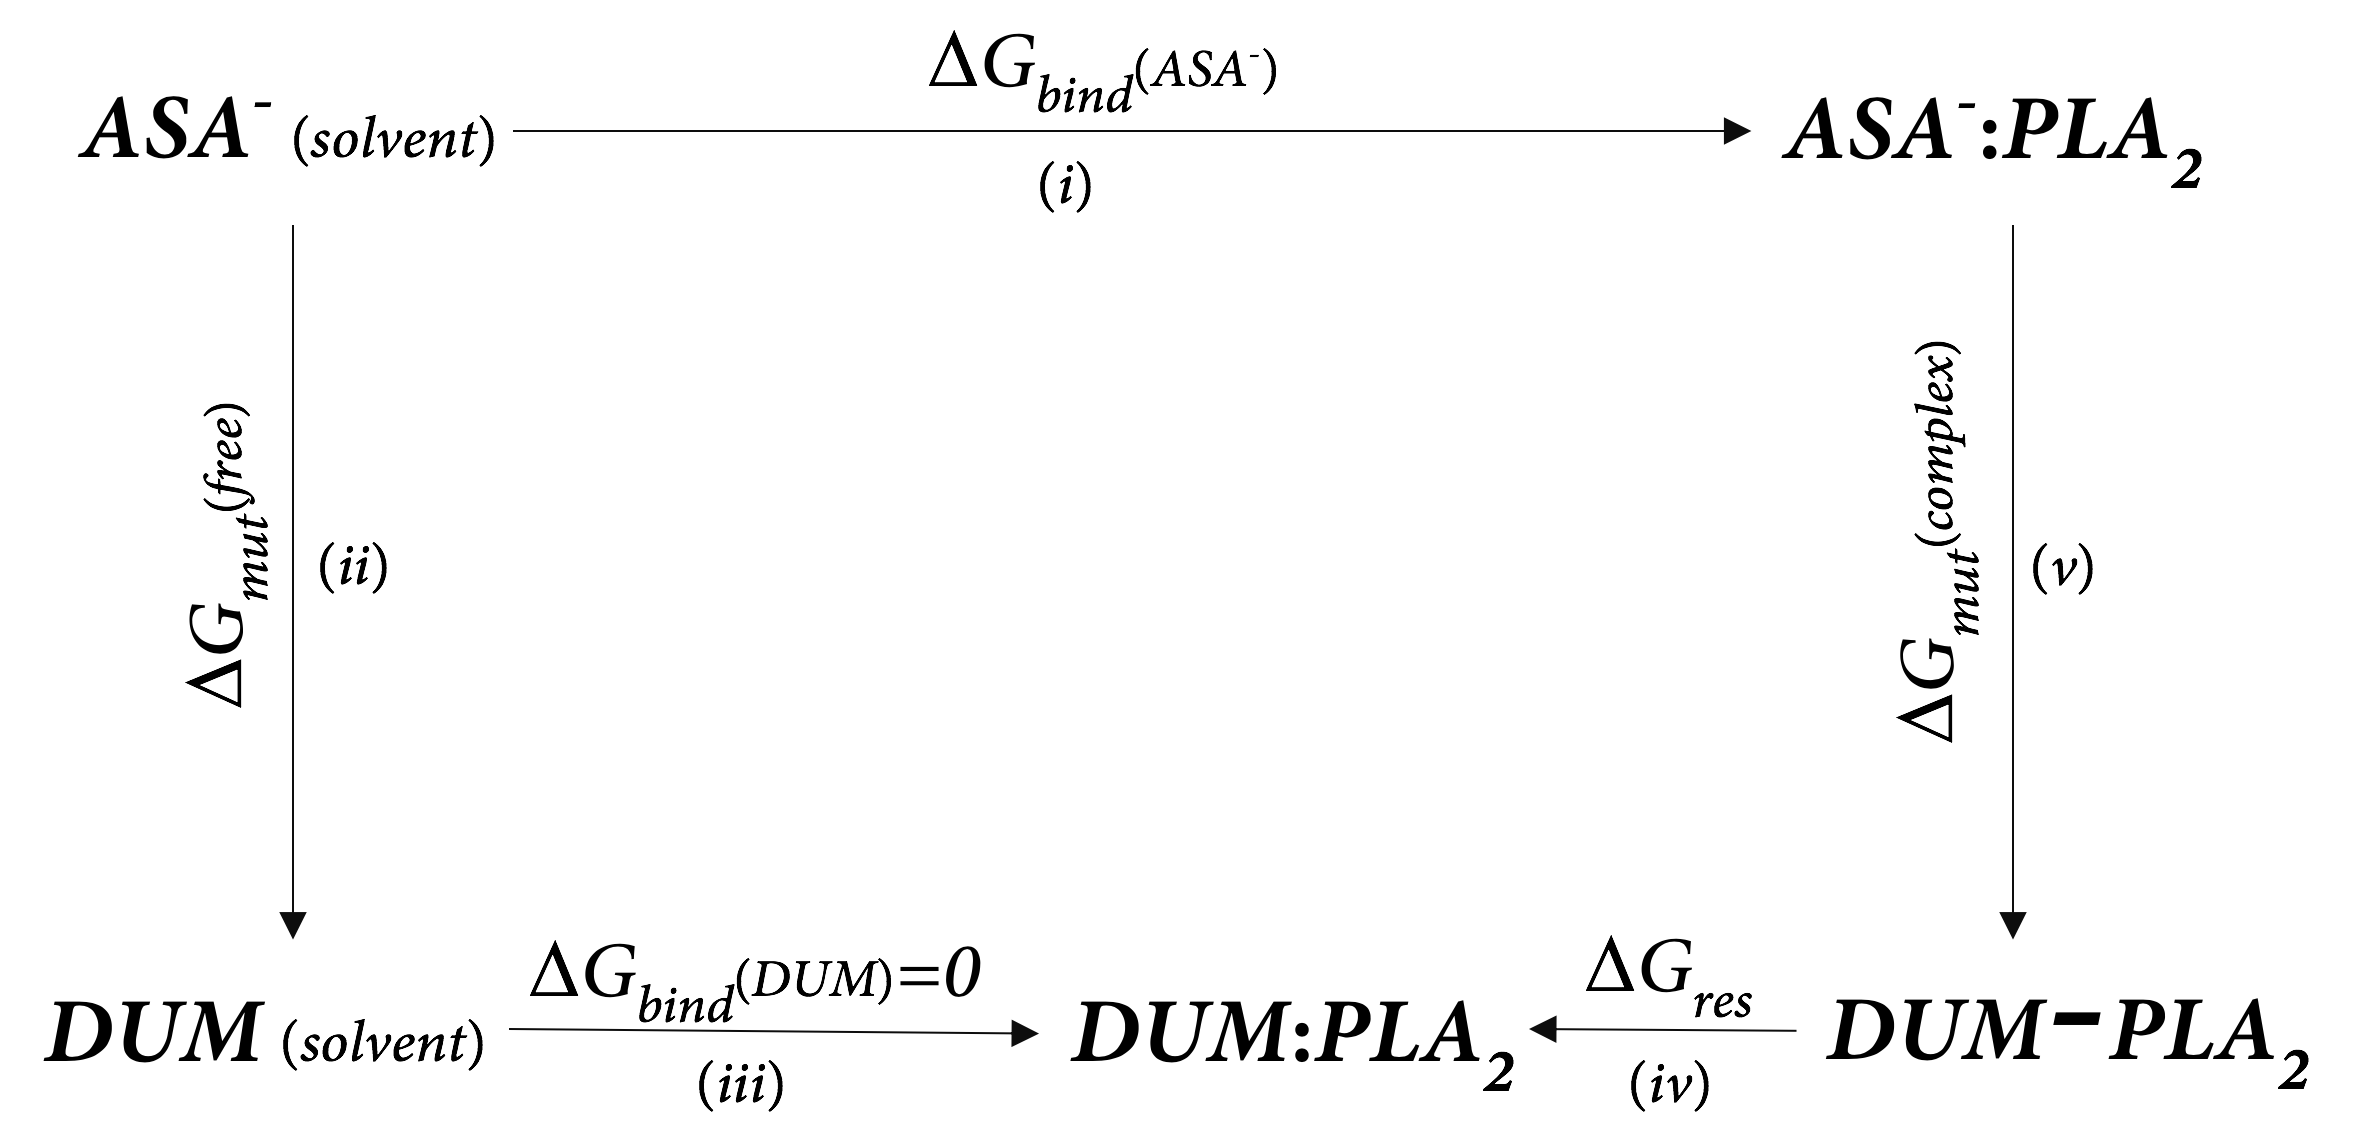
\includegraphics[scale=0.21]{../05_tutorial_02/figures/TC_ASA.png}
    \caption{Thermodynamic cycle for the calculation of the standard binding free energy of aspirin (ASA$^-$) binding to the protein phospholipase A$_2$ (PLA$_2$). ASA$^-$ is turned into a non-interacting dummy molecule (DUM), both in its complexed state (\textit{v}) and free in solution (\textit{ii}). The free energy of DUM binding to PLA$_2$ is zero (\textit{iii}). An intermediate state (DUM-PLA$_2$) is introduced by linking both binding partners with a harmonic distance restraint. The free energy contribution of this restraint can be calculated analytically (\textit{iv}) via equation \ref{disres}. The free energy differences of branches (\textit{ii}) and (\textit{v}) are determined via (extended) thermodynamic integration (TI), enabling the calculation of the standard binding free energy (\textit{i}).}
    \label{TC_ASA}
\end{figure}
%
In this tutorial we will calculate the standard binding free energy of aspirin (ASA) to the protein phospholipase A$_2$ (PLA$_2$) using the DDM and extended-thermodynamic interaction (X-TI)~\cite{X_TI}. 
For an application of X-TI and corrections of net-charge changes in current research see e.~g. Ref.~\cite{Ohlknecht_2020b}.

\subsubsection{Simulation setup}
Preparation of topologies and coordinate files, energy minimization, solvation in SPC water and the addition of counter ions as well as the setup of equilibrations and simulations can be performed in analogy to tutorial 1. The Cartesian coordinates for the enzyme phospholipase A$_2$ with bound acetyl salicylic acid (ASA) can be obtained from the Protein Databank with accession code 1OXR~\cite{Singh2005}.
The final equilibrated structures, \texttt{eq\_ASA\_Na\_7.cnf} and \texttt{eq\_PLA2\_ASA\_Ca\_2Na\_7.cnf}, are in subdirectories \texttt{eq/eq\_ASA} and \texttt{eq/eq\_PLA2\_ASA} of the directory \texttt{t\_02}. 

\subsubsection{Perturbation topology}
Go into the subdirectory \texttt{topo}. The topologies for the ligand (\texttt{ASA.top}) and the protein (\texttt{PLA2.top}) are already prepared. You can also find the combined topologies with sodium counter ions and a calcium ion that is important for the ligand binding (\texttt{ASA\_Na.top} and \texttt{PLA2\_ASA\_Ca\_2Na.top}). For ligand decoupling, the topology for ASA in the decoupled state (\texttt{DUM.top}) was generated by changing the integer atom code (\texttt{IAC}) to 22 corresponding to dummy type for all the atoms and setting all the charges to 0. The program \texttt{make\_pt\_top} can convert topologies from state A and B into a perturbation topology. The \texttt{PERTATOMPARAM} block lists all atoms with their respective force field parameters that will be alchemically perturbed during the simulation. 

\subsubsection{Distance restraints}
Distance restraints are introduced for the calcium ion to keep it bound in the active site. For this a distance restraint specification file \texttt{disres.dat} is set up in subdirectory \texttt{eq} containing the following block.
\begin{lstlisting}[columns=flexible]
DISTANCERESSPEC
# DISH  DISC
  0.1   0.153
# i     j  k  l  type i    j  k  l  type r0     w0    rah
  1208  0  0  0  0    309  0  0  0  0    0.223  1.0   0
  1208  0  0  0  0    321  0  0  0  0    0.235  1.0   0
  1208  0  0  0  0    339  0  0  0  0    0.246  1.0   0
  1208  0  0  0  0    489  0  0  0  0    0.255  1.0   0
  1208  0  0  0  0    490  0  0  0  0    0.248  1.0   0
END
\end{lstlisting}
The restraint is defined between the calcium ion and 5 atoms of residues coordinating the ion (3 amide oxygens and 2 carboxylate oxygens). \texttt{type} \texttt{0} is referring to explicit/real atoms. \texttt{r0} is the distance between two atoms in nm. The restraint is defined with a weight factor \texttt{w0} of 1 by which the distance restraint interaction term \texttt{CDIR} of the \texttt{DISTANCERES} block in the \texttt{imd}-file gets multiplied (force constant). The parameter \texttt{rah} controls the form and dimension of the restraint, here it is set to zero which corresponds to a full harmonic potential in $x$, $y$, $z$ dimensions. Parameters \texttt{DISH} and \texttt{DISC} are the hydrogen-carbon and carbon-carbon distances, respectively. GROMOS can also apply distance restraints on virtual or pseudo atoms by setting the appropriate type and a specification of additional atoms \texttt{j}, \texttt{k} and \texttt{l}. \\

To keep the ligand within the active site when getting decoupled, we gradually turn on a harmonic distance restraint simultaneously to the perturbation. Go into the subdirectory \texttt{DDM/md\_TI} where you will find the \texttt{disres.dat} file which contains an additional block.
\begin{lstlisting}
PERTDISRESSPEC
# DISH  DISC
0.1  0.153
# i j   k   l type i    j    k    l type n m Ar0  Aw0  Br0  Bw0 rah
 21 211 264 529 -1 1195 1199 1203 0 -1   0 0 0.0  0.0  0.0  1.0 0
END 
\end{lstlisting}

The distance restraint is defined between the centre of geometry (\texttt{type} \texttt{-1}) of 4 backbone atoms (\texttt{i}, \texttt{j}, \texttt{k} and \texttt{l}) of PLA$_2$ around the active site and the centre of geometry of 3 atoms of the ligand's benzene ring with a distance of zero (\texttt{A\_r0=B\_r0=0}). At state A the restraint is turned off (\texttt{A\_w0=0}), while at state B the restraint is retained with a weight factor of 1 (\texttt{B\_w0=1}). Parameters \texttt{n} and \texttt{m} control hidden 
restraints~\cite{Christen}. Parameters \texttt{DISH} and \texttt{DISC} are not relevant for the centre of geometry and this type of pseudo atoms.

\subsubsection{Extended-thermodynamic integration simulation} \label{chapt:exTI}
The thermodynamic integration approach uses the coupling parameter $\lambda$, which defines the system as a linear combination of the two end-states~\cite{kirkwood_TI}. The coupling parameter approach formulates the Hamiltonian of the system dependent on $\lambda$ by interpolating between the two states (scaling of force-field parameters). \\

\begin{align}
\label{equ:ext_ti}
V_{\text{nb}}(r_{ij},\lambda) = (1-\lambda)^n V^{\text{A}}(r_{ij},\lambda) + \lambda^n V^{\text{B}}(r_{ij},1-\lambda)
\end{align}
with
\begin{align}\begin{split}
V^{\text{X}}(r_{ij},\lambda) = \frac{C_{12}^{\text{X}}}{(\alpha_{\text{lj}}\lambda^2 C_{126}^{\text{X}} + r_{ij}^6)^2} - \frac{C_{6}^{\text{X}}}{\alpha_{\text{lj}}\lambda^2 C_{126}^{\text{X}} + r_{ij}^6} + \\
 \frac{q_i^{\text{X}} q_j^{\text{X}}}{4 \pi \epsilon_0} \left \lbrack \frac{1}{(\alpha_{\text{crf}}\lambda^2 + r_{ij}^2)^{1/2}} - \frac{1/2 C_{\text{rf}}r_{ij}^2}{(\alpha_{\text{crf}} \lambda^2 + R_{\text{rf}}^2)^{3/2}} - \frac{1 - 1/2C_{\text{rf}}}{R_{\text{rf}}} \right \rbrack
\end{split}\end{align}

\noindent where $C_{6}^{\text{X}}$, $C_{12}^{\text{X}}$, $q_i^{\text{X}}$ and $q_j^{\text{X}}$ are the Lennard-Jones parameters and partial charges for state X (A or B). $r_{ij}$ is the distance between particles $i$ and $j$, $C_{\text{rf}}$ and $R_{\text{rf}}$ are parameters of the electrostatic reaction field assumed outside the cutoff sphere \cite{Tironi1995}. 
$\alpha_{\text{crf}}$ and $\alpha_{\text{lj}}$ are soft-core parameters \cite{Beutler1994}. 

Go into the subdirectory \texttt{md\_TI}. The input files \texttt{md\_TI\_ASA\_Na.imd} and \texttt{md\_TI\_PLA2\_ASA\_Ca\_2Na.imd} contain two additional blocks that are relevant for the free energy calculations using X-TI integration. The \texttt{PERTURBATION} block controls the alchemical perturbation 
\begin{lstlisting}
PERTURBATION
#     NTG   NRDGL    RLAM   DLAMT 
        1       0     0.0     0.0 
#  ALPHLJ   ALPHC    NLAM  NSCALE 
      1.0     1.0       1       0 
END
\end{lstlisting}
\texttt{NTG} turns on the perturbation to calculate $\partial\mathcal{H}/\partial\lambda$ and \texttt{RLAM} is the initial value for $\lambda$. The initial value of $\lambda$ could also be read from the configuration when setting \texttt{NRDGL=1}. \texttt{RLAM} will be adjusted for several different $\lambda$ points using the jobs file \texttt{md\_TI.jobs}. \texttt{DLAMT} controls the increase of $\lambda$ with time. The parameters \texttt{ALPHLJ} and \texttt{ALPHC} are the soft-core parameters for Lennard-Jones ($\alpha_{\text{lj}}$) and Coulomb ($\alpha_{\text{crf}}$) interactions, respectively. \texttt{NLAM} controls the power dependence of the $\lambda$ coupling ($n$ in eq. \ref{equ:ext_ti}) and \texttt{NSCALE} the use of interaction scaling for complete energy groups.  

The \texttt{PRECALCLAM} block is relevant for the pre-calculation of intermediate non-simulated $\lambda$-points during the simulation as extension to standard TI. 
\begin{lstlisting}
PRECALCLAM
# NRLAM   MINLAM   MAXLAM
     81        0        1
END
\end{lstlisting}
With the settings in the above block, the energies and derivatives with respect to $\lambda$ will be calculated on-the-fly at 81 points ranging from $\lambda$=0 to $\lambda$=1, which results in $\lambda$-steps of 0.0125.


%%for PLA2-ASA with disres and new gromos binary
The simulation is defined in the jobs file \texttt{md\_TI.jobs}. Simulations will be performed at 11 equally spaced $\lambda$-points between $\lambda$=0 and $\lambda$=1 for 5 ns each in case of the complexed system, where ASA is bound to PLA$_2$. This system also requires the perturbed distance restraint. The simulations of ASA free in solution will also be performed at 11 $\lambda$-points each for 0.5 ns.   
Note that this tutorial can also be carried out using standard TI, in which case the \texttt{PRECALCLAM} block is not required. 
The choice of 11 equally spaced $\lambda$-points is typically a reasonable start, but it is recommended to adjust the number of points and the spacing according to the curvature and error estimates of $\partial\mathcal{H}/\partial\lambda$. 
In X-TI, adjustment is often not necessary, even fewer points are sufficient in some cases, but for standard TI usually more than 11 $\lambda$-points are needed. 
Therefore, we strongly recommend to use the \texttt{PRECALCLAM} block and take advantage of the pre-calculation of intermediate non-simulated $\lambda$-points and subsequent reweighting.
To run the two simulations, copy the argument files required by the \texttt{mk\_script} program into the two directories \texttt{md\_TI\_ASA} and \texttt{md\_TI\_PLA2\_ASA}, respectively, and adapt the paths before generating the job files with the \texttt{mk\_script} program and submitting the jobs to a cluster. If you prefer to continue directly, you will find the necessary energy and free energy trajectories in the subdirectories \texttt{L\_*}.

\subsubsection{Free energy analysis}
The free energies can be determined via extended-thermodynamic integration (X-TI)~\cite{X_TI} or the Bennett acceptance ratio (BAR) method~\cite{bar}. The raw data for both methods can be extracted from the energy and free energy trajectory files using the gromos++ program \texttt{ext\_ti\_ana}. 

Go into the subdirectory \texttt{DDM/ana\_TI/ana\_TI\_ASA} and run the program \texttt{ext\_TI\_ana} via the bash-script by typing
\begin{lstlisting}
$ ./ext_ti_ana_bar.sh
\end{lstlisting}
%
X-TI requires the pre-calculation of free energies at non-simulated points. Free energy derivatives at requested non-simulated $\lambda_{\text{P}}$ values can be reweighted to obtain ensemble averages for $\lambda_{\text{P}}$ from simulated $\lambda_{\text{S}}$ points. The predictions from multiple simulations at $\lambda_{\text{S}}$ points can be merged into a single TI profile by a linear reweighting scheme using the program \texttt{ext\_TI\_merge}. 
Run the program via the bash-script by typing
\begin{lstlisting}
$ ./ext_ti_merge.sh
\end{lstlisting}
%
The program calculates the integral of the final TI-curve using the trapezoidal rule in order to obtain the free energy estimate. The results of X-TI for both systems, ASA and PLA2\_ASA, are shown in Figure~\ref{TI_ASA}.  


BAR estimates free energies from the free energy differences between two adjacent $\lambda$ points $i$ and $j$, using
\begin{align}
\Delta G(\lambda_i \rightarrow \lambda_j) 
     = k_{\text{B}} T \ln \frac{\langle f(E(\lambda_i) - E(\lambda_j) + C)\rangle_{\lambda_j}}
          {\langle f(E(\lambda_j)-E(\lambda_i) - C )\rangle_{\lambda_i}}  + C
\end{align}
with
\begin{align}
f(x) = \frac{1}{1+\exp(x/k_{\text{B}} T)}
\end{align}
$C$ is determined iteratively to ensure that the two ensemble averages
from $\lambda_i$ and $\lambda_j$ are identical. To calculate error estimates, a
bootstrap sampling can be conducted. Run the program \texttt{bar} via
the bash-script by typing
\begin{lstlisting}
$ ./bar.sh 
\end{lstlisting}
%
BAR is computationally more efficient and converges relatively fast compared to regular TI. The efficiency of X-TI is comparable with the added advantage of a direct visualization of the entire free energy profile~\cite{Maurer}.

\begin{figure}[H]
    \centering
    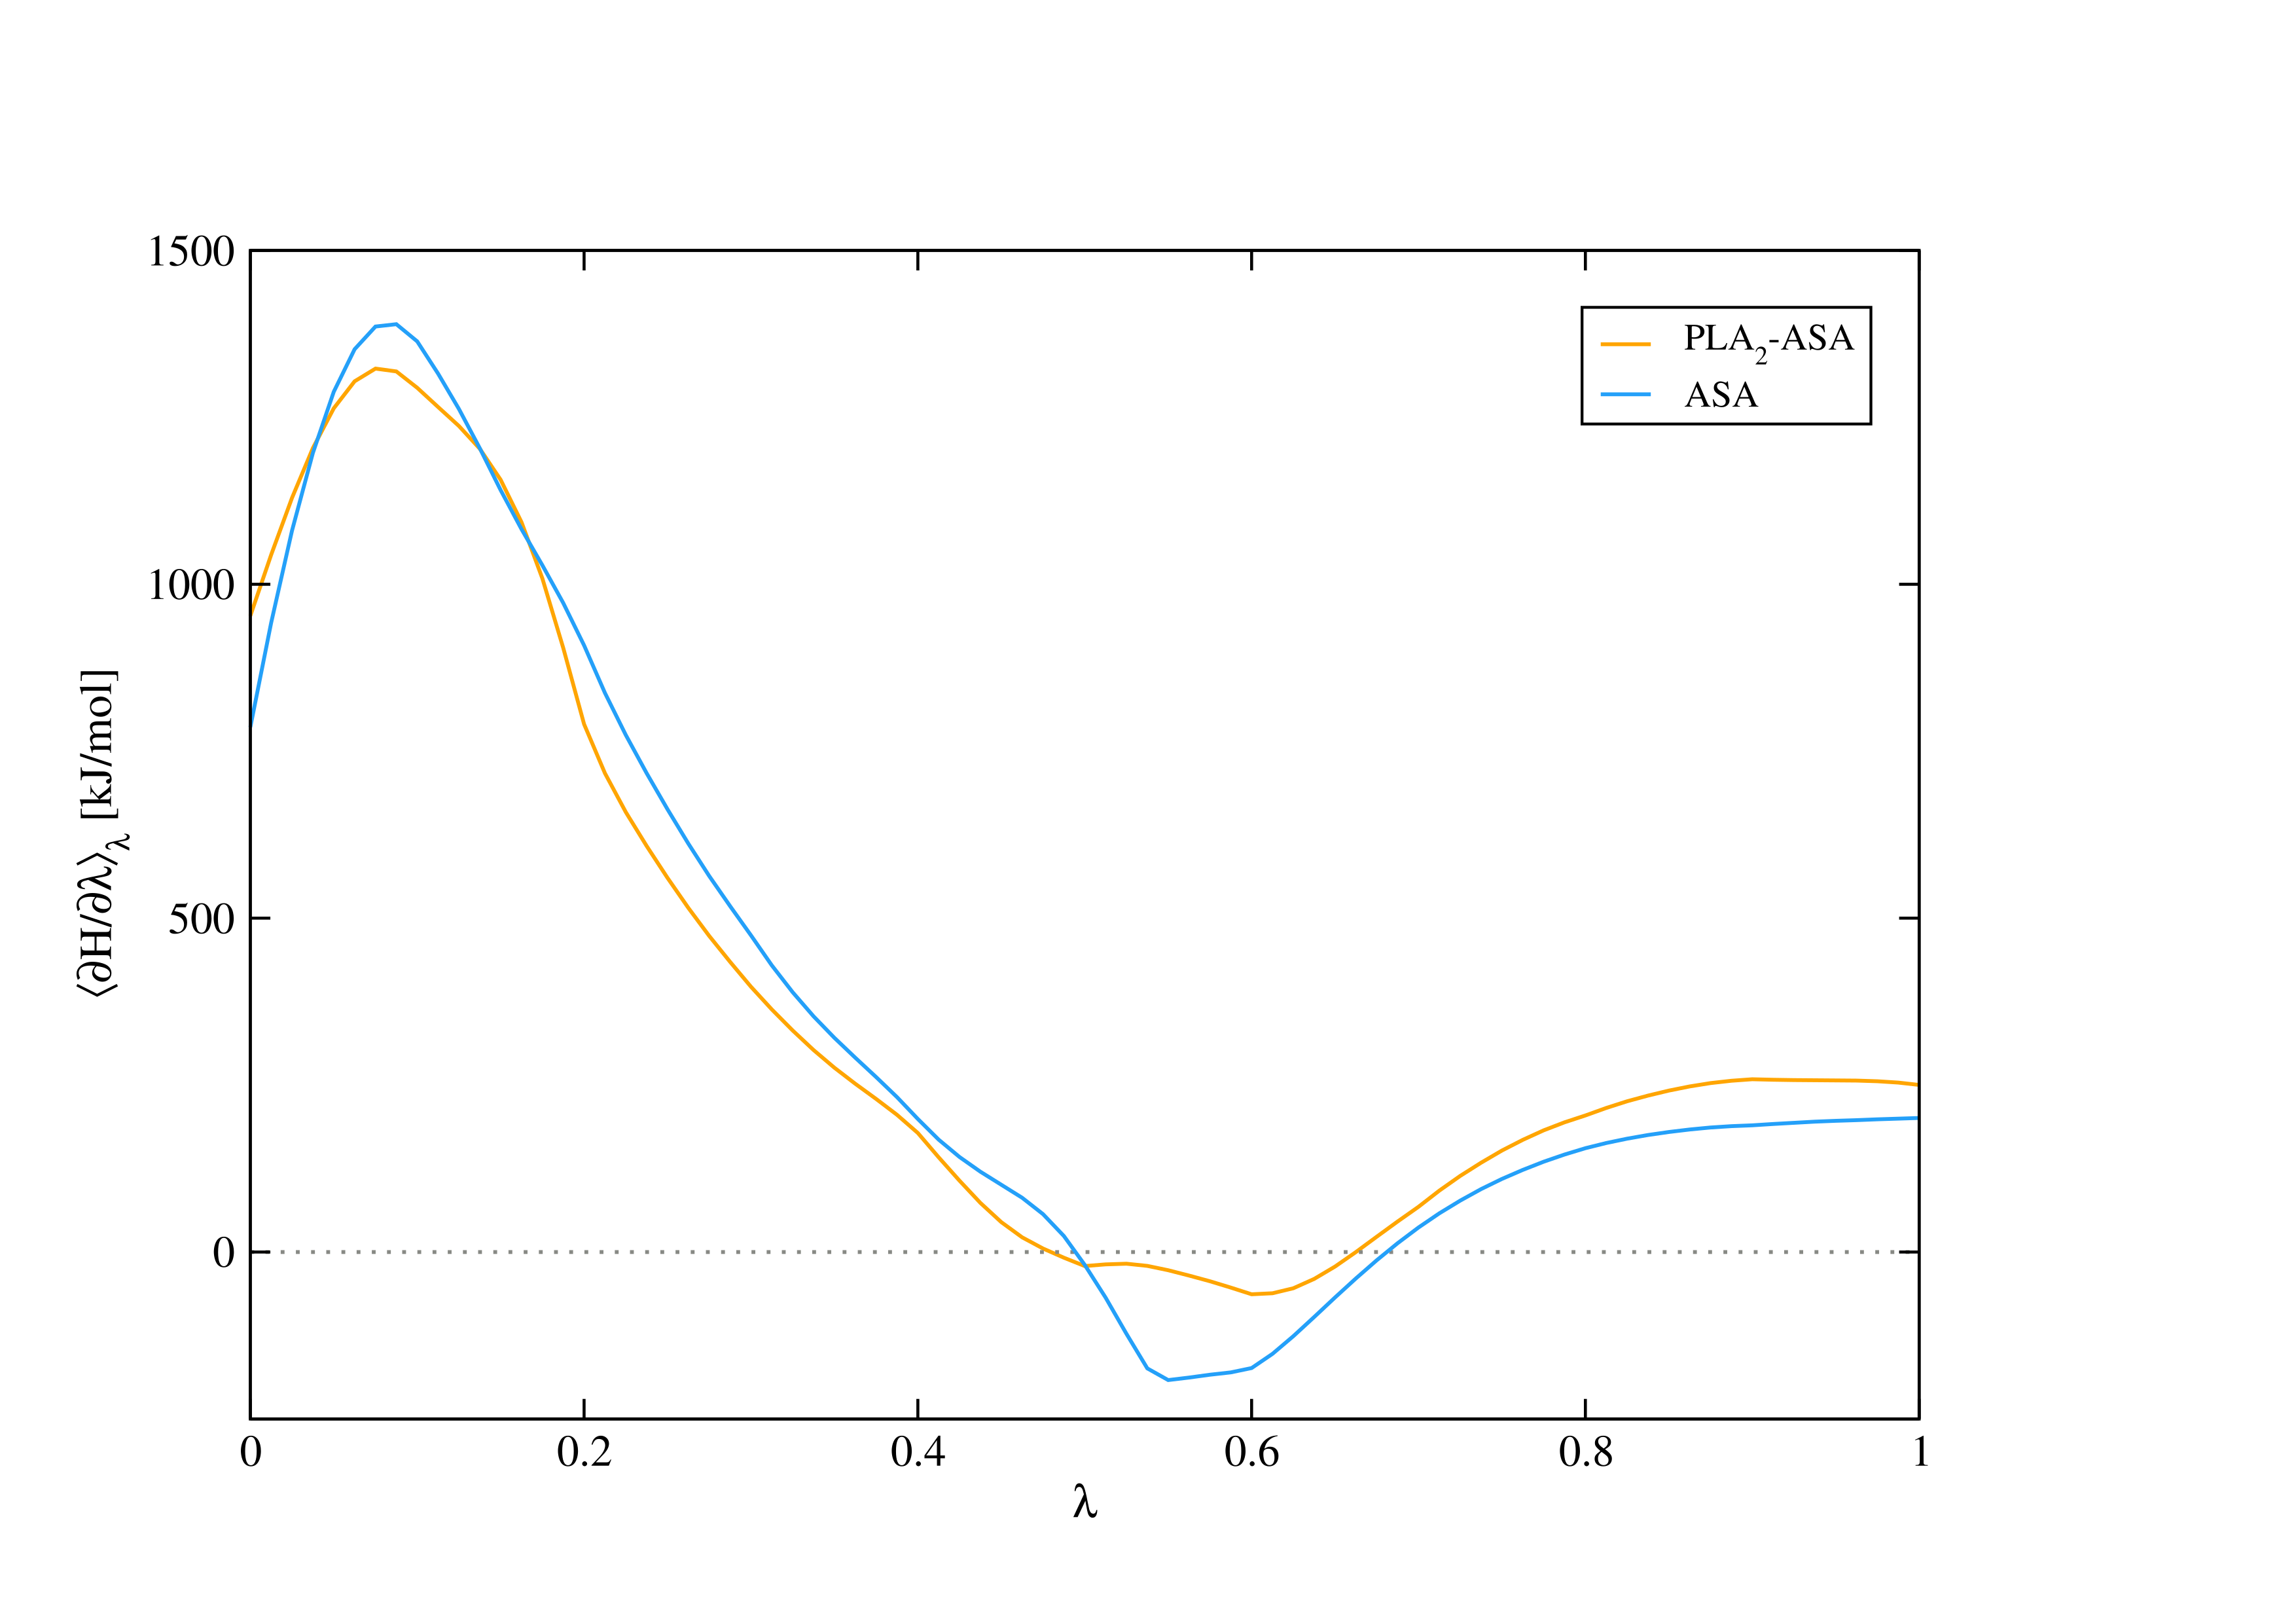
\includegraphics[scale=0.3]{../05_tutorial_02/figures/ana_TI.png}
    \caption{The reweighted property $\left<\frac{\partial\mathcal{H}}{\partial\lambda}\right>$ for $\lambda$=0 to $\lambda$=1 for both systems ASA and PLA$_2$\_ASA.}
    \label{TI_ASA}
\end{figure}

\subsubsection{Thermodynamic cycle}
The free energy of binding is determined according to the thermodynamic cycle shown in Figure~\ref{TC_ASA} as
\begin{align}\begin{split}
& \Delta G_{\text{bind}}(\text{ASA}^-)= \\ 
& \Delta G_{\text{mut}}(\text{free})+\Delta G_{\text{bind}}(\text{DUM})-\Delta G_{\text{res}}-\Delta G_{\text{mut}}(\text{complex})
\end{split}\end{align}
%
The free energy associated with the removal of the restraint ($\Delta G_{\text{res}}$) for a dummy particle can be calculated analytically, including a standard state correction~\cite{Roux, Boresch}: 
\begin{align} \label{disres}
    \Delta G_{\text{res}} = -k_{\text{B}}T \ln\frac{V^{\circ}}{\Big(2\pi k_{\text{B}}T/K\Big)^{3/2}}
\end{align}
where $K$ is the force constant of the harmonic distance restraint and $V^{\circ}$ is the accessible solution volume corresponding to the standard-state definition. For a molar reference concentration it is given by $V^{\circ}=1.661$~nm$^3$.
Equation \ref{disres} corrects for restricted mobility and can be derived from the partition function associated with the restraining potential energy function, 
given that the restraint is so strong that the integration volume can be extended to the entire space~\cite{Gebhardt2016}.

\subsubsection{Correction terms for net-charge changes}
Due to finite box sizes, periodic boundary conditions and
simplifications in the calculations of the electrostatic interactions,
the calculated free energies are artifacted. In the following
paragraphs, we will refer to these energies as raw free energies. We
will quantify and correct these artifacted components using a
free energy correction $\Delta G_{\text{cor}}$ to yield methodology-independent
values $\Delta G$ as
\begin{align}
    \Delta G = \Delta G_{\text{raw}} + \Delta G_{\text{cor}}
\end{align}
%
Analogous to Reif and Oostenbrink~\cite{Reif2014}, $\Delta G_{\text{cor}}$ is a
combination of multiple free energy corrections for a spurious
solvent-polarization ($\Delta G_{\text{pol}}$), the impracticality
of
calculating the zero of the potential under periodic boundary
conditions using discrete solvent molecules ($\Delta G_{\text{dsm}}$) and
artifacted direct interactions between the ligand and the host
molecule ($\Delta G_{\text{dir}}$). The free energy correction is calculated
as
\begin{align} \label{equ:corrected_free_energy}
  \Delta G_{\text{cor}} = \Delta G_{\text{pol}} + \Delta G_{\text{dir}} + \Delta G_{\text{dsm}}
\end{align}
%
These three correction terms will be calculated in the following
paragraphs. A general scheme about the calculation of the corrections
based on $\lambda$-generated trajectories can be found in
Figure~\ref{fig:correction_scheme}~\cite{Ohlknecht2020}. 
Note that within this tutorial, only the information needed for the
practical part is provided, further details about the theory can be
found elsewhere~\cite{ReifBook2011,Kastenholz2006_I,Reif2014}. The set
of the three correction terms needs to be calculated for both branches of
the thermodynamic cycle. Have a look into the directory
\texttt{corrections}. It contains subdirectories for Aspirin free in
solution and the complex of Phospholipase A2 with Aspirin. The
correction procedure will only be explained for Aspirin free in
solution, the procedure for the complex is similar. Go into the
directory \texttt{corrections/ASA}. First, we need to create a set of
topologies for intermediate states. These topologies will have full,
unperturbed VdW parameters but charges that scale with $\lambda$.  Go
further into the subdirectory \texttt{correction\_topologies}. The
python script \texttt{interpolate\_topocharges.py} takes three input
parameters: topologies at states A and B and a specific
$\lambda$-value. A new topology with charges that correspond exactly
to the given $\lambda$-value is written out. All other parameters
remain unperturbed and are taken from topology A. We do not have to use
it directly but can use the bash script
\texttt{do\_interpolate\_topocharges.bash} instead. It creates six
topologies at equidistant $\lambda$-points. These will be used for the
individual correction terms explained in the following paragraphs.

\begin{figure}[H]
    \centering
    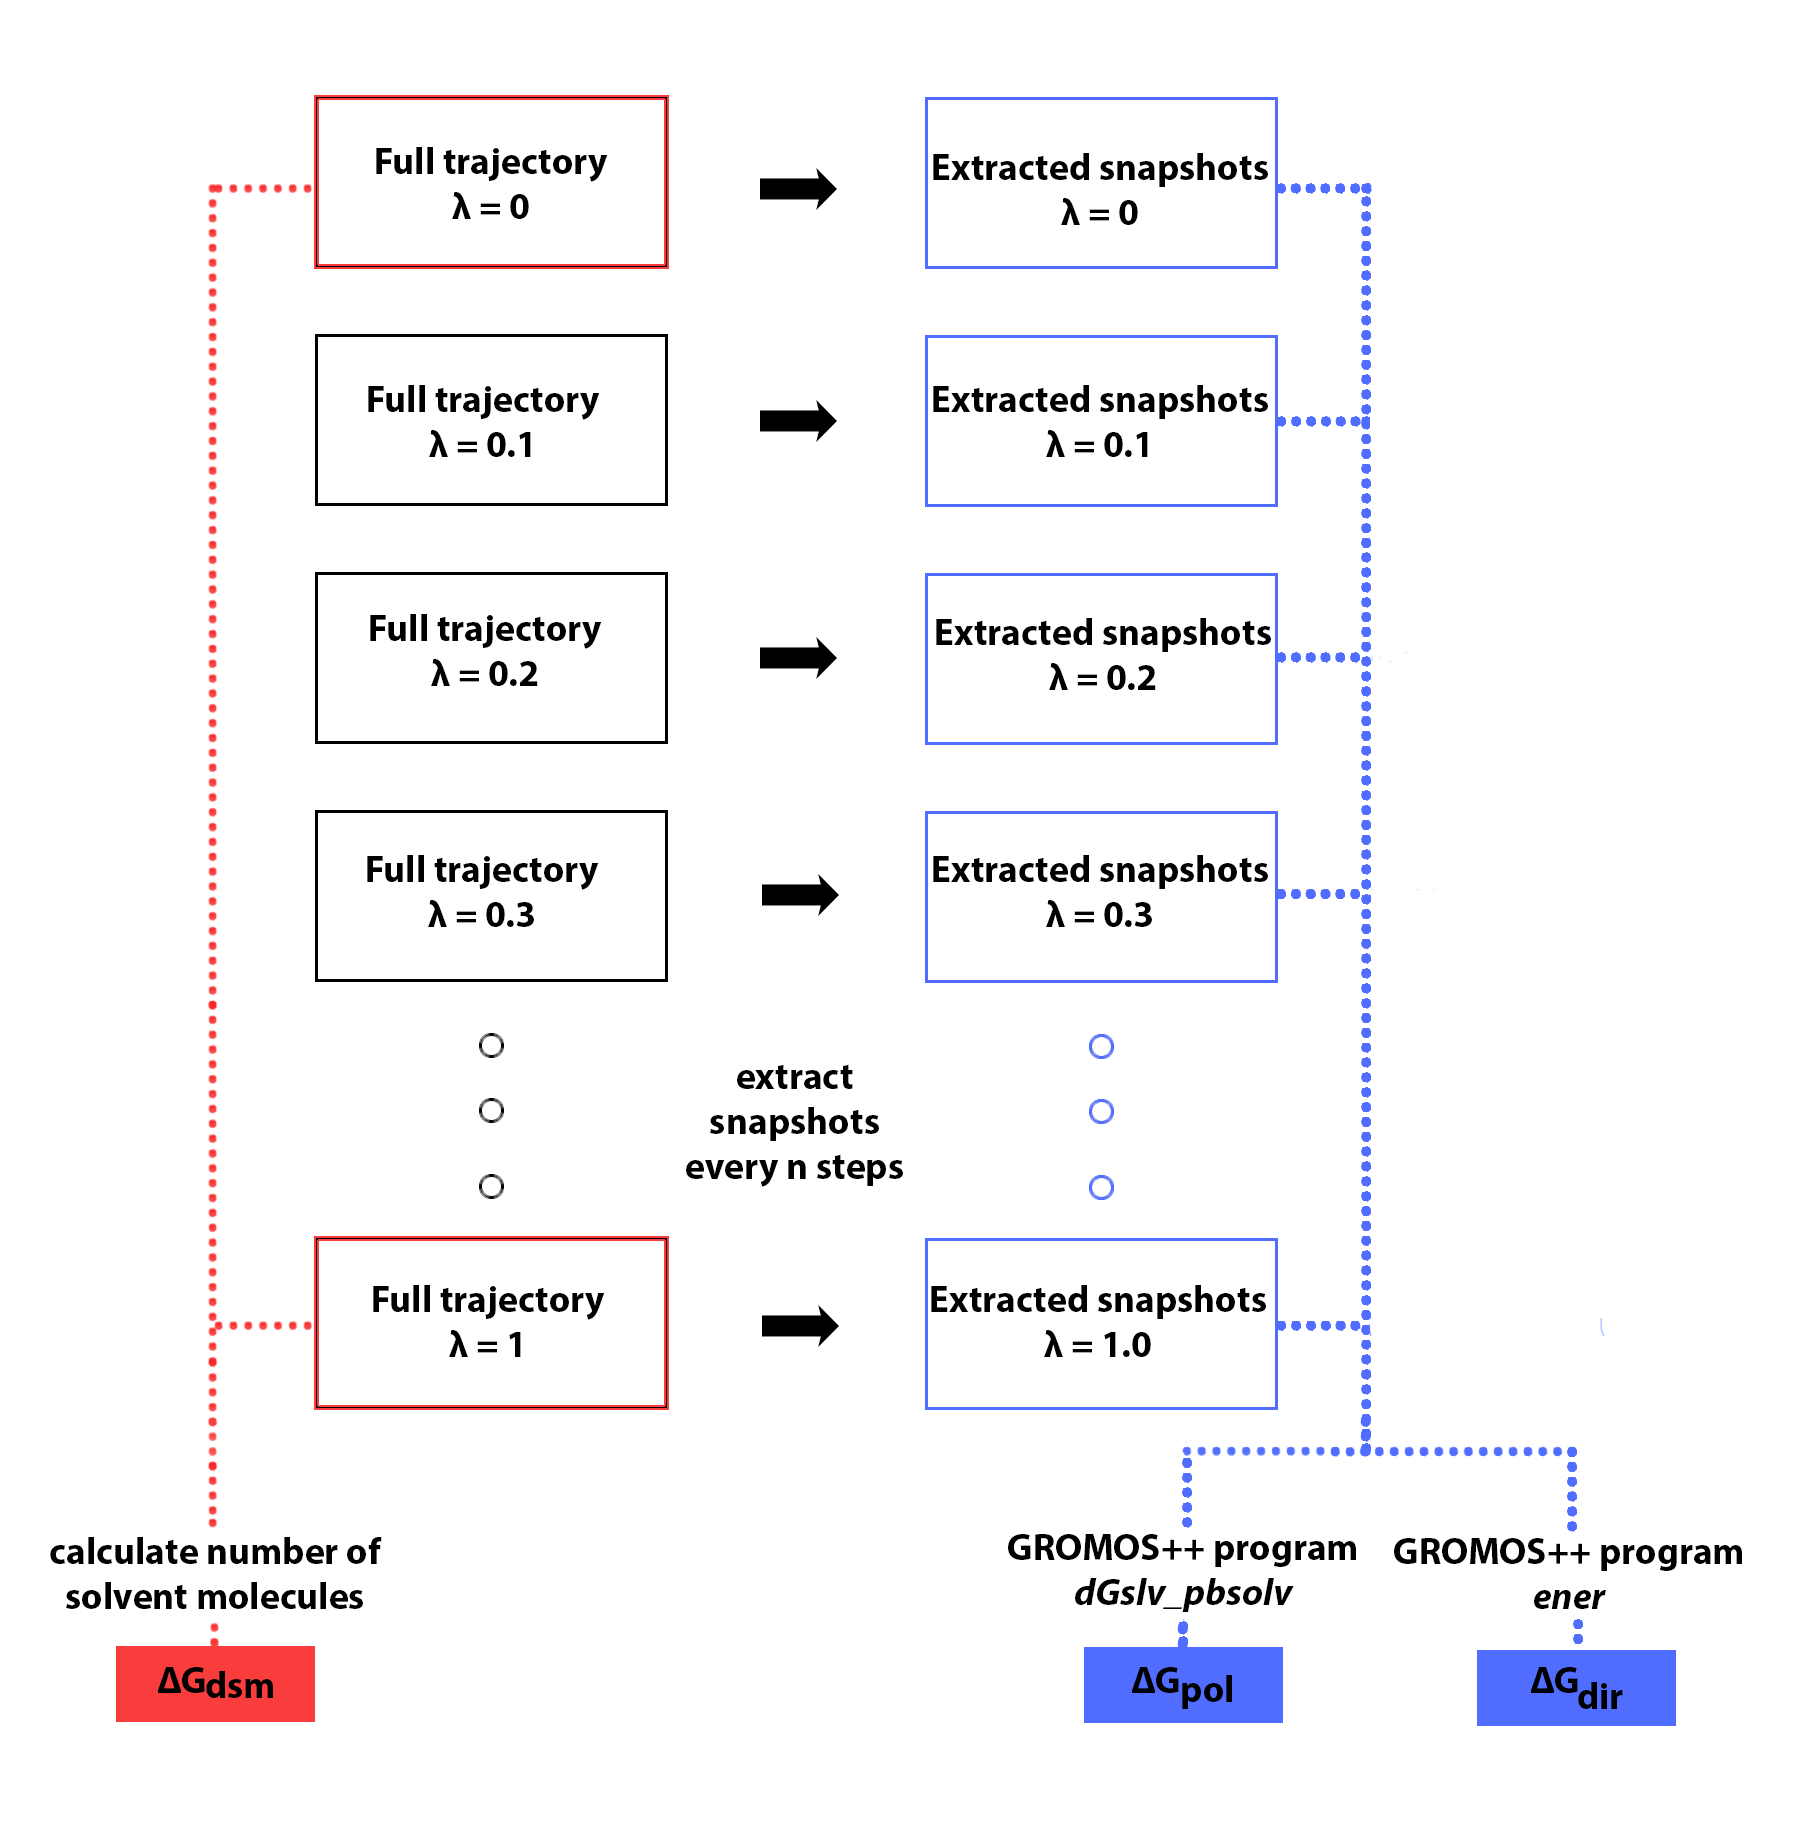
\includegraphics[scale=0.14]{../05_tutorial_02/figures/general_application_corrections.png}
    \caption{Schematic representation of the corrections. $\Delta G_{\text{dsm}}$ is
      calculated over full trajectories of the end states (however, if one of the end states has zero charges, it can be skipped). $\Delta G_{\text{pol}}$ and $\Delta G_{\text{dir}}$ are both calculated on individual snapshots
      only. In this tutorial, only the final snapshots of 6 chosen $\lambda$-points are used for these calculations.}
    \label{fig:correction_scheme}
\end{figure}


\subsubsection{Solvent polarisation}
First, we calculate the correction estimate $\Delta G_{\text{pol}}$ for the
spurious solvent polarisation. We will use a set of
continuum-electrostatics calculations on configurations extracted from
trajectories that were sampled at different $\lambda$ points. For each of
these configurations, the electrostatic potential at the atom sites of the
Aspirin molecule will be calculated twice - using a cutoff scheme with
a reaction-field contribution under periodic boundary conditions and
using full Coulombic charges under non-periodic boundary
conditions. The integrated differences between both
potentials will give an estimate of $\Delta G_{\text{pol}}$, which can be directly
applied to the raw free energies that were calculated in the
simulation. Note that for the sake of simplicity, in this tutorial we
will use only the last configurations of six $\lambda$-generated
trajectories. However, when used for ``real'' research questions, a
more complete set of configurations should be analysed in order to achieve
more reliable results.

Go into the subdirectory \texttt{corrections/ASA/dGpol}. It
contains argument files for the GROMOS++ program
\texttt{dGslv\_pbsolv}. There are six argument files for six different
$\lambda$ points.
% and one additional argument file that uses a snapshot that was generated with full charges but is re-analyzed with zero charges. 
Since the continuum-electrostatics calculations are
computationally demanding, the output files are already
provided. However, if you prefer to run the continuum-electrostatics
calculations yourself, you can run them by typing
\begin{lstlisting}
$ dGslv_pbsolv @f dGslv_pbsolv_L_0.0.arg > dGslv_pbsolv_L_0.0.out
$ dGslv_pbsolv @f dGslv_pbsolv_L_0.2.arg > dGslv_pbsolv_L_0.2.out
...
$ dGslv_pbsolv @f dGslv_pbsolv_L_1.0.arg > dGslv_pbsolv_L_1.0.out
\end{lstlisting}
%$ dGslv_pbsolv @f ASA_Na_L_0.0_no_charges.arg > ASA_Na_L_0.0_no_charges.out
%
Let's have a look at one of the output files. It contains four rows for
the individual atoms of the charged acetyl group
of the Aspirin molecule. There are several
columns. Next to basic information for the individual atoms, there are
six columns with potentials created under non-periodic boundary
conditions in solvation (NPBC\_SLV), non-periodic boundary conditions
in vacuum (NPBC\_VAC), periodic boundary conditions in solvation
(PBC\_SLV), periodic boundary conditions in vacuum (PBC\_VAC), a fast
Fourier transform result for the lattice-summation method under
periodic boundary conditions (FFT\_LS\_PBC) and a fast Fourier
transform result for the reaction-field method under periodic boundary
conditions (FFT\_RF\_PBC).  The potential that has to be integrated
over $\lambda$ reads (NPBC\_SLV - NPBC\_VAC) - (PBC\_SLV - PBC\_VAC) -
(FFT\_LS\_PBC - FFT\_RF\_PBC). Note that the last term has to be used
only if a cutoff scheme with reaction field contribution was applied
in the simulation. You can simply use the script
\texttt{integrate.py}. Type
\begin{lstlisting}
$ ./integrate.py
\end{lstlisting}
We are interested in the result NPBC - PBC, which is the correction term $\Delta G_{\text{pol}}$.
%12.3 kJ/mol. 

\subsubsection{Direct ligand-protein interactions}
In the actual MD simulation, the interaction between the ligand and
the protein atoms was calculated by a cutoff scheme with a reaction
field contribution. A correct scheme would involve no cutoff and
purely Coulombic interactions. $\Delta
G_{\text{dir}}$ accounts for the difference between the simulated and the
real case. Note that in order to minimize the dependence of the
correction terms on the conformations of the molecules the same
configurations have to be used for $\Delta
G_{\text{dir}}$ that were used for the calculations of $\Delta
G_{\text{pol}}$. Go into the subdirectory
\texttt{corrections/ASA/dGdir}. It contains argument files for the
GROMOS++ program \texttt{ener}. There are 12 argument files for six
different $\lambda$-points,
one for Coulombic interactions under non-periodic boundary conditions
(NPBC) and one for Coulomb/Reaction-field interactions under periodic
boundary conditions (PBC). You can use the provided output files or
generate them yourself by typing
\begin{lstlisting}
$ ener @f ener_PBC_L_0.0.arg > ener_PBC_L_0.0.out
$ ener @f ener_NPBC_L_0.0.arg > ener_NPBC_L_0.0.out
$ ener @f ener_PBC_L_0.2.arg > ener_PBC_L_0.2.out
...
$ ener @f ener_NPBC_L_1.0.arg > ener_NPBC_L_1.0.out
\end{lstlisting}
%
We are interested in the integrated energies NPBC-PBC. You can do it
yourself or use a provided Python script. Simply type
\begin{lstlisting}
$ ./integrate.py 
\end{lstlisting}
The integrated result is the correction term $\Delta G_{\text{dir}}$. %should be around -9.1 kJ/mol.

\subsubsection{Potential from discrete solvent molecules}
Another artifact stems from the impossibility of calculating the
absolute zero potential in a periodic simulation box and the
convention to average the solvent-generated potential over the
exterior and the interior of the solvent molecules. As a consequence,
the calculated potential differs from the ``real'' potential by an
offset. For a rigid solvent model with a single van der Waals
interaction site and any scheme relying on molecular-cutoff truncation
based on this specific site, it can be shown that this offset is
related to the quadrupole moment trace of the solvent model used. The
free energy correction is furthermore proportional to the
water-molecule density inside the box (LS - lattice summation schemes)
or within the cutoff radius (cutoff schemes with reaction-field
correction - RF) and reads
\begin{equation}
  \Delta G_{\text{dsm}}(\text{LS}) = -N_{\text{A}} (6 \epsilon_0)^{-1} \gamma_{\text{s}} \Delta Q N_{\text{S}} V_{\text{B}}^{-1}
\end{equation}
for the LS scheme and
\begin{equation} \label{equ:dsm}
  \Delta G_{\text{dsm}}(\text{RF}) = -N_{\text{A}} (6 \epsilon_0)^{-1} \frac{2 (\epsilon_{\text{RF}}-1)}{2\epsilon_{\text{RF}}+1} \gamma_{\text{s}} \sum_{i=1}^n \Delta q_i \left\langle N_{\text{S}}(R_{\text{C},i})\right\rangle V_{\text{C}}^{-1}
\end{equation}
for the RF scheme, where $N_{\text{A}}$ is the Avogadro constant, $\epsilon_0$
is the vacuum dielectric permittivity, $\epsilon_{\text{RF}}$ is the (relative)
reaction-field dielectric permittivity, $\Delta Q$ is the net-charge
change in the system, $\Delta q_i$ is the net-charge change of the perturbed atom $i$, $N_{\text{S}}$ is the number of solvent molecules in the
box, $\left\langle N_{\text{S}}(R_{\text{C},i})\right\rangle$ is the average number of
solvent molecules in the cutoff sphere of the perturbed atom i, $V_{\text{B}}$ is the volume of the
computational box and $V_{\text{C}}$ is the volume of the cutoff
sphere. $\gamma_{\text{s}}$ is the quadrupole moment trace relative to the van
der Waals interaction site. Values for typically used water models can be found in
table \ref{tab:quadrupole_moments}. Hint: the reaction-field permittivity used in the simulations can be found in the \texttt{NONBONDED} block in one of the \texttt{imd} files, parameter \texttt{EPSRF}.

\begin{table}[h]
  \center
  \caption{ Quadrupole-moment traces [e nm$^2$] for typical solvent models}
  \label{tab:quadrupole_moments}
  \begin{tabular}{ l  c  }
    \hline
    \textbf{model} & $\gamma_{\text{s}}$ \\ 
    \hline
    SPC~\cite{Berendsen1981} & 0.008200 \\
    SPC/E~\cite{Berendsen1987} & 0.008476 \\
    TIP3P~\cite{Jorgensen1983} & 0.007641 \\
    TIP4P~\cite{Jorgensen1983} & 0.009295 \\
    TIP5P~\cite{Mahoney2000} & 0.002054 \\
    ST2~\cite{Stillinger1974} & 0.001754 \\
    \hline
  \end{tabular}
\end{table}
%
Go into the subdirectory \texttt{corrections/ASA/dGdsm}. First, we need
to calculate the average number of water molecules in the cutoff
sphere that was used in the simulation. We will calculate this number
using a radial distribution function (rdf) over the trajectory that
was generated with full charges on the perturbed atoms. The argument
file for the GROMOS++ program \texttt{rdf} is already provided, 
as is the output file for the case your simulation did not finish yet.
You can run \texttt{rdf} by typing
\begin{lstlisting}
$ rdf @f rdf.arg > rdf.out 
\end{lstlisting}
The output file contains the densities of water particles as function of
the distance of all the perturbed atoms. 
%----------------------------------------------------------------------------------
%To obtain the
%total number of water molecules, these densities need to be integrated
%over the distance and multiplied by the water number density
%$\rho = N/V_{\text{B}}$ in the simulation box. The latter can be found by looking
%into one of the configuration files - the POSITION block contains the
%number of solvent molecules and the GENBOX block provides the box
%dimensions.  The integral over the rdf can be calculated using the
%provided Python script. You can simply run it by
%typing %The calculated water number density in the box should be roughly 32.4.
%\begin{lstlisting}
%$ ./integrate.py
%\end{lstlisting}
%%The calculated total amount of water molecules in the cutoff sphere
%%should be about 370.
%Equation \ref{equ:dsm} then gives the final
%correction term $\Delta G_{\text{dsm}}$. %which should be roughly 77.5 kJ/mol
%---------------------------------------------------------------------------------------------------
To obtain the
total number of water molecules, these densities need to be integrated
over the distance and multiplied by the water number density
$\rho = N/V_{\text{B}}$ in the simulation box. Equation \ref{equ:dsm} then gives the final correction term $\Delta G_{\text{dsm}}$ . You can calculate it by typing
\begin{lstlisting}
$ ./integrate.py
\end{lstlisting} 
This script reads the file \texttt{rdf.out} as well as \texttt{system.info} that contains relevant information about the box size, the cutoff, the correction field and the solvent model.    
Relevant information about the box size can be found by looking
into one of the configuration files - the \texttt{POSITION} block contains the
number of solvent molecules and the \texttt{GENBOX} block provides the box
dimensions.  Settings for the electrostatics can be found in the \texttt{NONBONDED} block in the \texttt{imd} files. 


\subsubsection{Corrected results}
Above, the three correction terms for Aspirin free in solution were
calculated. According to equation \ref{equ:corrected_free_energy}, the
sum of these three correction terms constitutes the total correction
for this branch of the thermodynamic cycle. The same set of correction terms has to be
calculated for the ligand bound to the host (directory \texttt{corrections/PLA2\_ASA}). Both corrections
can be directly added to the raw free energies to yield
methodologically independent results (see table \ref{tab:results}). The final calculated estimate $\Delta G^{\circ}_{\text{bind}} = \Delta G(\text{PLA}_2\_\text{ASA}) - \Delta G(\text{ASA}) = -32.3$ kJ/mol agrees 
quite well with the experimentally determined estimate of $\Delta G_{\text{bind,exp}} = -29.6$ kJ/mol~\cite{Singh2005}.

\begin{table}[h]
  \center
  \caption{ Results from Double Decoupling with corrections. All values are reported in kJ/mol.}
  \label{tab:results}
  \begin{tabular}{ @{}l c@{\phantom{~~}} c c c c@{\phantom{~}} c@{}}
    \hline
    \textbf{System} & $\Delta G_{\text{raw}}$ & $\Delta G_{\text{res}}$ & $\Delta G_{\text{pol}}$ & $\Delta G_{\text{dir}}$ & $\Delta G_{\text{dsm}}$ & $\Delta G$ \\
    \hline
    ASA & -371.2 & - & 12.3 & -9.1 & 77.5 & -290.5 \\
    PLA$_2$\_ASA & -383.2 & 18.2 & -13.3 & 23.4 & 32.1 & -322.8 \\
    \hline
  \end{tabular}
\end{table}

\subsubsection{Common errors}
\textbf{[Note:} Please document frequently occurring errors, including a clear descriptive title for each error and a brief explanation of how it occurs, how to resolve it, and how to prevent it.\textbf{]}

\paragraph{Error}
cause, indicators, solution, prevention, tips,...




% Tutorial 03

\subsection{Tutorial 3: Using HREMD and distance-field}
Another way to calculate the binding free energy of a ligand to a protein is to pull the ligand out of the active site. 
There are several methods available to perform such calculations, however, most of them require the \textit{a priori} knowledge of the dissociation path. 
Even if the dissociation path is determined during the simulation, it is often assumed that it is linear, or that only a single dissocation path exists. 
For an accurate estimate of the binding free energy the simulations should be performed such that the binding and unbinding of the ligand can be sampled reversibly.
In this tutorial we will use the distance-field (DF) distance as the reaction coordinate and combine this with Hamiltonian-replica-exchange molecular dynamics (HREMD) simulations \cite{deRuiter_2013}.
The advantage of the DF distance is that we will be able to pull the ligand back into the active site, even if it moved to the other side of the protein. 
The HREMD simulations allow for multiple paths to be sampled reversibly.

\subsubsection{Preparations}
As in the tutorial above, we will use the PLA$_2$ - ASA complex as a test system. 
The preparation of the topology, coordinates, the energy minimization and the equilibration of the system are very similar to the tutorial above. 
The only difference is that we will use a larger cubic box to allow the ligand to move freely in the solvent. 
The final equilibrated structure can be found in the directory \texttt{eq} with the name \texttt{eq\_PLA2\_ASA\_Ca\_2Na\_7.cnf}.

\subsubsection{Slow-growth}
In order to get some initial coordinates for each of the replicas of the HREMD simulations, we will perform a short slowgrowth simulation where the ligand is pulled out of the active site in a non-equilibrium manner. 
The exact pulling speed and force constant are not relevant in this case as we are not trying to calculate the binding free energy from the slow-growth simulations. 
It is, however, important that the structure of the protein does not get disrupted during this initial simulation. 
The slow-growth simulation is started from the final configuration of the equilibration. 
Go to the directory \texttt{slowgrowth} and have a look at the \texttt{PERTURBATION} block in the input file \texttt{slowgrowth.imd}. 
\begin{lstlisting}
PERTURBATION
#     NTG   NRDGL    RLAM   DLAMT
        1       0     0.0   0.001
#  ALPHLJ   ALPHC    NLAM  NSCALE
      0.0     0.0       1       0
END
\end{lstlisting}
With \texttt{NTG} set to \texttt{1}, you specify that a free energy calculation will be performed. 
The starting $\lambda$ point \texttt{RLAM} is set to \texttt{0}. With each timestep during the simulation, $\lambda$ will be increased. The rate of increase in ps$^{-1}$ is set to \texttt{DLAMT = 0.001}. 
Together with \texttt{NSTLIM = 500000} (from the \texttt{STEP} block) and an integration time step of 0.002~ps this results in a simulation of 1ns where $\lambda$ is continuously changed from 0 to 1. 
\texttt{ALPHLJ} and \texttt{ALPHC} are the softness parameters of the Lennard-Jones and Coulombic interactions, respectively. 
These are set to 0 here, because we are not changing any nonbonded interactions, only distance restraints. 
In addition to that, we have to specify which kind of restraints will be used. In this case we will use distance-field distance restraints:
\begin{lstlisting}
DISTANCEFIELD
# NTDFR
      1
#  GRID PROTEINOFFSET PROTEINCUTOFF PROTECT
    0.2       15          0.2             0
# UPDATE  SMOOTH   RL   NTWDF     PRINTGRID
    100        1  1.0    1000             0
END
\end{lstlisting}
With \texttt{NTDFR} set to \texttt{1}, we turn on distance-field (DF) restraining during the simulation. Typically the grid size (\texttt{GRID}) for the DF calculation is set to 0.2~nm. 
\texttt{PROTEINOFFSET} is the penalty which is added to the DF distance if the path crosses the host. 
This value has to be large enough, such that paths through the protein always result in larger DF distances than around the protein. Here we have chosen \texttt{PROTEINOFFSET = 15}. 
\texttt{PROTEINCUTOFF = 0.2} determines that any grid point which is within 0.2 nm of a protein atom will be flagged as protein. 
In cases where the binding site is quite small, it can happen that the zero distance point is often flagged as protein, in these cases it might be necessary to use \texttt{PROTECT > 0}. 
This is the radius around the zero-distance point in which a grid point will not be flagged as protein. For our simulation, we will leave this value at \texttt{0}. 

In order to speed up the simulation, the grid is calculated only every \texttt{UPDATE = 100} steps. 
The \texttt{SMOOTH} parameter is used to prevent very large forces acting at the surface of the protein due to the large penalties. 
With each smoothening step the non-protein grid points are identified which have a direct neighbouring grid point flagged as protein. 
These are on the edge of the protein and we will recalculate their DF distance but now without the protein penalty. 
This removes the large forces pointing away from the protein, but because the smoothening steps are performed after the updating step, they do not influence the optimal route. 
We will set the number of smoothening rounds to \texttt{1}. Forces change linearly for distances larger than 1 nm as set by \texttt{RL}. 
We will write DF distances and forces to an external file (special trajectory file, *.trs) every \texttt{NTWDF = 1000} steps. We will not print the grid to the final configuration, so we use \texttt{PRINTGRID=0}. 
The definition of the distance restraint that will be modified during the slow-growth simulation, is specified in the distance restraint specification file \texttt{disres.dat}. 
There are two blocks in this file. 
The first one, \texttt{DISTANCERESSPEC} specifies the distance restraints between the Ca$^{2+}$ ion and its surrounding residues, which prevents the Ca$^{2+}$ from drifting away. 
The second block \texttt{PERTDFRESSPEC} specifies the perturbed distance-field restraints. 
\begin{lstlisting}
PERTDFRESSPEC
# DISH  DISC
  0.1   0.153
# PROTEINATOMS  A_R0  K_A  B_R0  K_B  M  N
          1190   0.0  500   5.0  500  0  0
#  TYPE_I  NUM_I ATOM_I[0] .. ATOM_I[NUM_I]
       -1      7    16 190 249 312 486 632 1208
#  TYPE_J  NUM_J ATOM_J[0] .. ATOM_J[NUM_J]
       -1      2  1194 1203
END
\end{lstlisting}
\texttt{DISH = 0.1} specifies the carbon - hydrogen distance and \texttt{DISC = 0.153} specifies the carbon-carbon distance in nm. 
These are used to compute the position of some types of pseudo or virtual atoms, respectively, from the positions of explicitly represented atoms.
\texttt{PROTEINATOMS} specifies the last atom number of the protein which will be used to flag protein atoms. 
\texttt{A\_R0} and \texttt{B\_R0} are the restraining distances in nm at \texttt{$\lambda$ = 0} and \texttt{$\lambda$ = 1}, respectively. 
We will use a force constant of 500 kJ mol$^{-1}$ nm$^{-2}$ which remains the same upon changing $\lambda$ (\texttt{K\_A = K\_B = 500}). 
We will not use hidden distance restraints, so \texttt{M = N = 0}. 

The distance between pseudo atom \texttt{i} and pseudo atom \texttt{j} will be restrained, where pseudo atom \texttt{i} is defined as the center of geometry of 7 atoms (\texttt{NUM\_I = 7}) with atom numbers 16, 190, 249, 312, 486, 632 and 1208. 
These atom numbers correspond to the $C_{\alpha}$ atoms of residues L2, W18, A22, C28, D48, Y63 (residue numbers according to the topology) and the calcium ion. 
Pseudo atom \texttt{j} is the center of geometry of atoms C2 and C7 (topology names) of the aspirin ligand. 
All input files are now prepared and we can generate the run file with:
\begin{lstlisting}
$ mk_script @f mk_script.arg
\end{lstlisting}
Make sure the generated \texttt{slowgrowth\_PLA2\_ASA\_1.run} file is ready to be submitted to a cluster. 
After running the slow-growth simulation, we can analyze the system by using \texttt{trs\_ana}. 
We will use this program to read out the DF distances and forces from the special trajectory, \texttt{*.trs}, file. An example of the argument file is prepared in \texttt{trs\_ana.arg}. 
You can run the program with 
\begin{lstlisting}
$ trs_ana @f trs_ana.arg
\end{lstlisting}
The DF distance as a function of time is written out to the file \texttt{df\_dist.dat}. Have a look at the file with e.g. Xmgrace and make sure no sudden jumps are present. 
We also need to make sure that the protein was not disrupted during the pulling process. For this, calculate the root-mean-square deviation (RMSD) as a function of time with
\begin{lstlisting}
$ rmsd @f rmsd_bb.arg > rmsd_bb.dat
$ rmsd @f rmsd_all.arg > rmsd_all.dat
\end{lstlisting}
Have a look at the RMSD of the backbone atoms (\texttt{rmsd\_bb.dat}) as well as for all protein atoms (\texttt{rmsd\_all.dat}). 
When both the \texttt{df\_dist.dat} and the RMSD plots look normal, we can continue to prepare the starting structures for the replica-exchange simulations. 
If not, the slow-growth simulation should be performed again with some variables modified.
For example, you can decrease \texttt{DLAMT} (and increase \texttt{NSTLIM} accordingly) in order to pull slower. 
Changing the force constant of the DF restraints (\texttt{K\_A} and \texttt{K\_B} in the \texttt{PERTDFRESSPEC} block) or choosing different atoms to apply the DF restraints to can also help to avoid any disruption of the protein.

\subsubsection{Hamiltonian-replica-exchange simulations}
One of the first choices that we have to make when starting a HREMD simulation, is how many replicas will be used. 
For performance issues it is best to keep the number of replicas equal to the number of CPUs available (preferably on a single computational node). 
In the prepared example, we used 24 replicas. Have a look at the prepared input file for the replica-exchange simulation (\texttt{HREMD.imd} in the directory \texttt{HREMD}). 
You will find that the \texttt{PERTURBATION} block is still present, but with \texttt{DLAMT} now set to \texttt{0}. 
This means we are still calculating free energies, but we are no longer changing the $\lambda$ parameter during a single simulation. 
The \texttt{DISTANCEFIELD} block is pretty much unchanged, apart from \texttt{NTWDF} because we will write out the DF data more often. You will also find an additional block:
\begin{lstlisting}
REPLICA
# NRET
  1
# RET(1..NRET)
  298.0
# LRESCALE
  0
# NRELAM
  24
# RELAM(1..NRELAM)
 0.0000 0.0435 0.0870 0.1304 0.1739 0.2174 0.2609 0.3043 0.3478 0.3913 0.4348 0.4783 0.5217 0.5652 0.6087 0.6522 0.6957 0.7391 0.7826 0.8261 0.8696 0.9130 0.9565 1.0000
# RETS(1..NRELAM)
 0.002  0.002  0.002  0.002  0.002  0.002  0.002  0.002  0.002  0.002  0.002  0.002  0.002  0.002  0.002  0.002  0.002  0.002  0.002  0.002  0.002  0.002  0.002  0.002
# NERTRIAL
  100
# NREQUIL
  0
# CONT
  1
END
\end{lstlisting}
Because we will perform Hamiltonian-replica-exchange and not temperature replica exchange, the number of replica exchange temperatures are set to \texttt{NRET=1}. 
We thus also only have one \texttt{RET} value which is the temperature of each replica, in this case equal to 298~K. 
We do not need to scale temperatures after exchange trials, so \texttt{LRESCALE=0}. \texttt{NRELAM} is the number of replica-exchange lambda values, which is set to 24 here. 
For each of the replicas you have to specify at which $\lambda$ value it should be simulated. These values are given at \texttt{RELAM}. 
We do not know the optimal spread of the $\lambda$ values of the replicas before actually running the simulations, so as an initial guess we just spread them evenly between $\lambda$ = 0 and 1. 
We will keep the standard timestep of 0.002 ps for each $\lambda$-replica, as given by \texttt{RETS}. 
In order to keep the simulation time per run short, we set the number of exchange trials per run to \texttt{NERTRIAL=100}. 
Prolonging the simulations can then be done by performing multiple runs sequentially. 
\texttt{NREQUIL} sets the number of exchange periods for equilibration, during which no switches between the replicas are allowed. 
This would be especially benificial if you start the HREMD simulations from a single configuration and you need time to equilibrate. 
Since we start from multiple configurations which are close to their respective $\lambda$ values, we will set this to 0. 
\texttt{CONT=1}, as we start from multiple configuration files, instead from a single configuration.
The next step will be to select the appropriate configurations from the slow-growth simulation as initial configurations for each of the replicas.

The script \texttt{write\_start\_files.py} in the directory \texttt{starting\_coordinates} will help with this. 
The program will find the $\lambda$ values of the replicas, look for the DF restraint in the PERTDFRESSPEC block in the distance restraints file and determine the restraining distances for each of the replicas from this information.
It will then search for the frame in the slow-growth simulation which has a DF distance which is closest to the restraining distance of this replica.
This frame will be written to a separate file for each of the replicas, named \texttt{start\_\{X\}.cnf}, where \texttt{X} will be the replica number. 
An example argument file is provided which lists the topology of the system, the DF distances over time of the slow-growth simulation (\texttt{df\_dist.dat}), the coordinate trajectory from the slow-growth simulation, the HREMD input file and the distance restraint specification file as will be used for the HREMD simulation. To run the script:
\begin{lstlisting}
$ ./write_start_files.py @write_start_files.arg 
\end{lstlisting}
The starting coordinates for the HREMD simulation are now available and we can prepare the run files with \texttt{mk\_script}:
\begin{lstlisting}
$ mk_script @f mk_script.arg
\end{lstlisting}
The HREMD simulations are split into quite a few runs, in order to prevent an extremely long single simulation. 
Go to the first directory, \texttt{run1} and submit \texttt{HREMD\_1.run} to a computer cluster, preferable with the same number of CPUs as we have replicas, which would be 24 in the prepared example. 

\subsubsection{Analysis of HREMD}
All analyses for HREMD simulations will be performed in the subfolder \texttt{analysis}. 
In order to make sure the choice of replicas is appropriate, we will analyze whether there were sufficient switches between the replicas. This can be done already after only a few runs have finished. 
The switching information of the replicas is written out to the \texttt{replica.dat} file for each of the runs separately. 
You can combine them into a single file by using the provided script:
\begin{lstlisting}
$ ./gather_replica_data.sh [nr_runs] [nr_trials]
\end{lstlisting}
Here, you need to replace [nr\_runs] with the number of runs which have been performed already and [nr\_trials] with the number of exchange trials per run, which was set to 100 in the example files.
This script results in the file \texttt{replica\_all.dat}. The switches of the replicas can now be visualized by running
\begin{lstlisting}
$ ./rep_ana_mpi.py replica_all.dat
\end{lstlisting}
The resulting \texttt{rep\_change.out} file can be opened with \linebreak Xmgrace. An example of such file is shown in  Figure~\ref{rep_change}.

\begin{figure}[H]
\centering
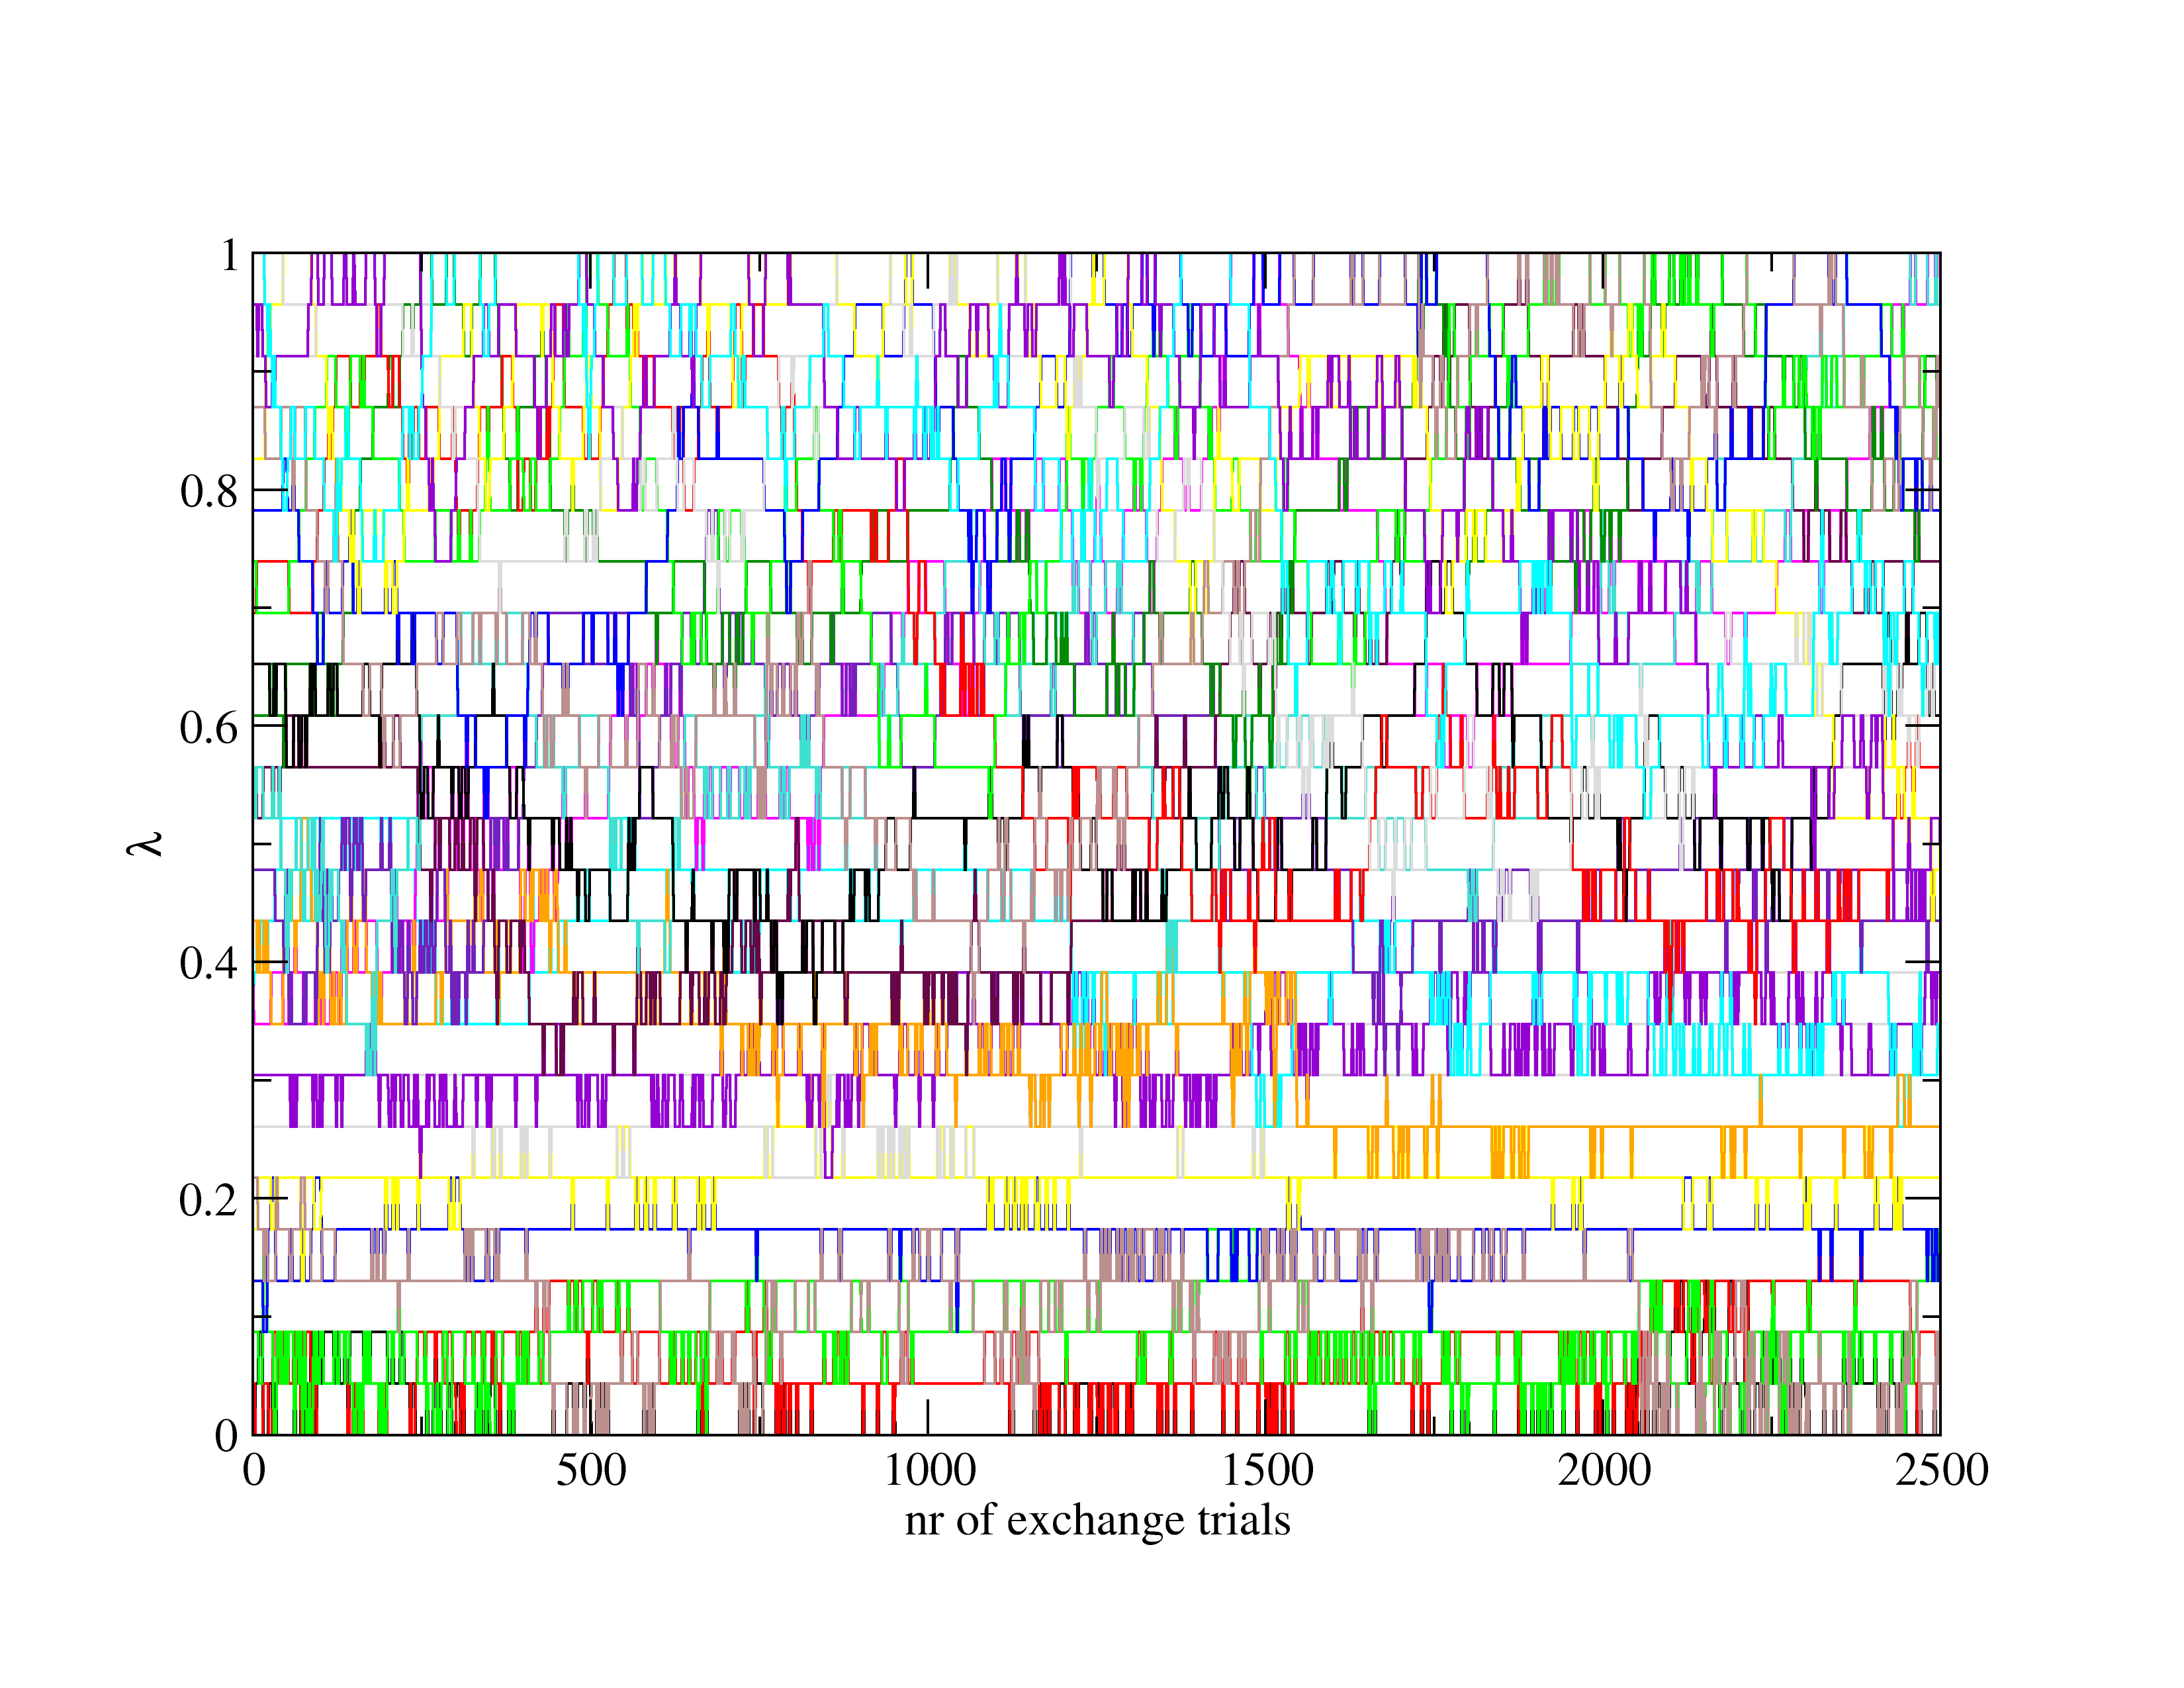
\includegraphics[scale=.3]{../06_tutorial_03/figures/rep_change}
\caption{Replica exchanges during time. Different colors represent different replicas.}
\label{rep_change}
\end{figure}

In case there is a pair of $\lambda$ points for which not enough switches are occurring, you have two options to resolve this. 
You can either insert another $\lambda$ point or make the difference between the $\lambda$ points smaller. 
The former option is maybe quicker to set up, but requires longer simulation time because of the additional replica. 
The latter option does not require more replicas, but it is not guaranteed that your small change improves the switching probabilities and that you do not introduce another region of low switching probability due to the change.
Of course you can also use more elaborate methods to optimize the $\lambda$-spacing \cite{Hritz_2007}.

If you are happy with the switching probabilities, you can start preparing for the calculation of the Free Energy Curve (FEC).
First, we have to write out the measured DF distances for each of the replicas. Then we calculate the distributions of these and on this data we can perform the weighted histogram analysis method (WHAM) which will result in the FEC.
We will again use the program \texttt{trs\_ana} to extract the DF distance from the special trajectories (\texttt{*trs.gz}). 
A small script is provided which runs this program for each of the replicas, thereby collecting data from each of the runs.

\begin{lstlisting}
$ ./do_all_trs_ana.sh [nr_runs] [nr_replicas]
\end{lstlisting}
This will generate a subdirectory called \texttt{df\_dist} which then contains \texttt{df\_dist\_X.dat} files for each replica X. 
From these distance files, we will first generate the distributions, which can then be used to determine the FEC by applying WHAM. 
The program \texttt{tcf} can generate distributions for each of the \texttt{df\_dist} files. 
We will set the boundaries to 0 and 5 nm (the same range as the restraining distances) and use 200 bins. 
Especially the boundaries should be adapted when working on different systems. 
Again, a small script is prepared which will perform the program \texttt{tcf} on each of the replicas:

\begin{lstlisting}
$ ./do_tcf.sh [nr_replicas]
\end{lstlisting}
One should always check whether the distributions at adjacent $\lambda$-values are sufficiently overlapping and whether the individual distributions are sufficiently sampled.
We can then determine the FEC $F(r)$ by using the WHAM program. 
Note that the FEC contains the Jacobian contribution, whereas a PMF does not \cite{Trzesniak_2007}. 
As input parameters, the WHAM program needs the temperature of the simulation, the restraining distance for each replica and the force constant of the restraints. 
All this information is read from the \texttt{HREMD.imd} and \texttt{disres.dat} files as specified in the \texttt{do\_wham.sh} file:
\begin{lstlisting}
$ ./do_wham.sh
\end{lstlisting}
This script also moves the final FEC on the y-axis such that its minimum is placed at 0 kJ/mol.
The file \texttt{wham\_FEC\_200bins\_5000iter\_min0.dat} now contains the final FEC, which is shown in Fig.~\ref{FEC}. As you can see, the curve is not completely flat at larger distances, but is rather noisy. Ideally, you would have to change the spacing of the replicas, add more replicas in the unbound range, or lower the maximum distance which you restrain such that the replicas are placed more densely in the unbound range. 
However, we can still see where the plateau of the unbound range is, so we will go ahead with the calculation of the binding free energy.

\begin{figure}[H]
\centering
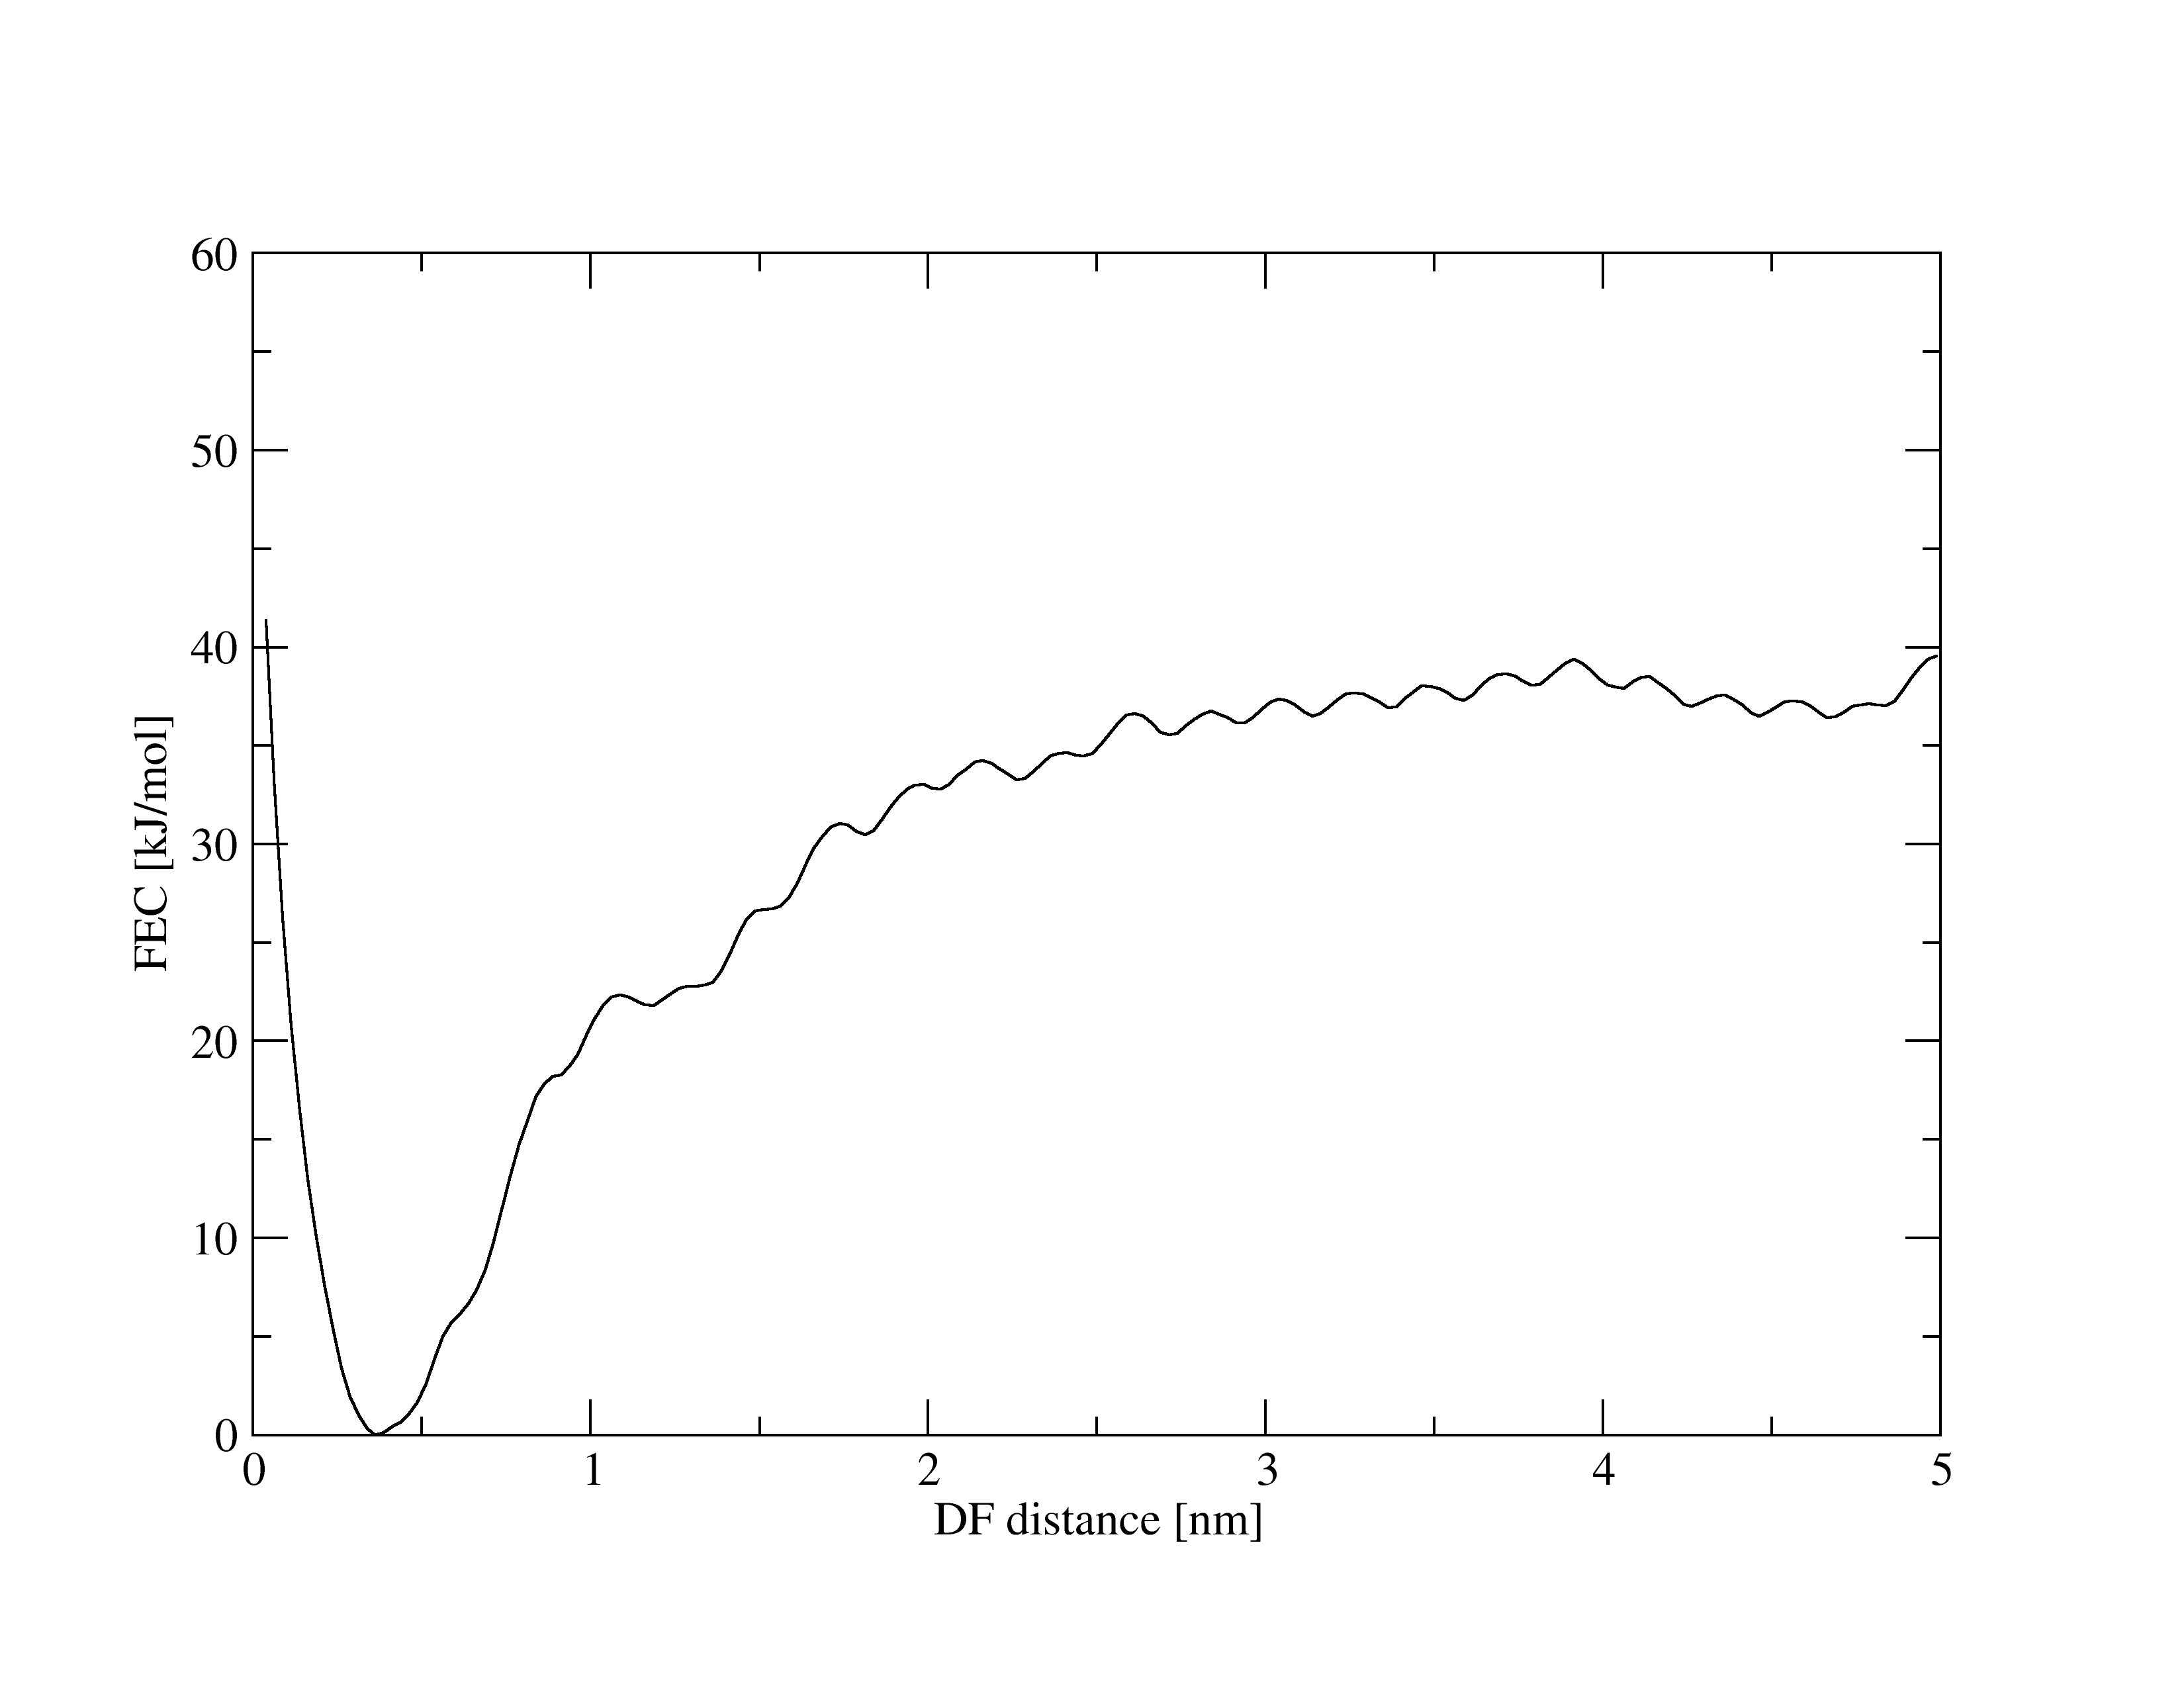
\includegraphics[scale=.3]{../06_tutorial_03/figures/FEC}
\caption{Free Energy Curve (FEC) along the DF distance as obtained from HREMD simulations, for the PLA2-ASA system.}
\label{FEC}
\end{figure}

\subsubsection{Calculation of binding free energy}

To derive the binding free energy from the FEC in Fig.~\ref{FEC} we cannot simply take the value of $\Delta G$ at the plateau around the unbound state. We will need to integrate the bound and unbound ranges of the FEC and we will need to include the standard state correction of 
\begin{equation}
\Delta G_{\text{std}} = -k_{\text{B}}T \ln \left (\frac{V_{\text{u}}}{V^{\circ}} \right )
\end{equation}
Here, $V^{\circ}$ is the standard state volume of 1.661 nm$^3$ and $V_{\text{u}}$ is the unbound volume which is sampled by the ligand in the unbound range.
This range is defined by the plateau observed in the FEC curve.  

In order to determine $V_{\text{u}}$ we need to select the configurations of the trajectory which contributed to the plateau range of the FEC. 
In this example, the plateau can be observed between 3 and 5 nm. 
The script \texttt{select\_frames\_unbound\_region.sh} (which you can find in the subdirectory \texttt{unboundVolume}) will select the appropriate frames by reading in the \texttt{df\_dist\_X.dat} files which were generated using \texttt{do\_all\_trs\_ana.sh}.
Since the DF distances are written out every 50 steps (\texttt{NTWDF=50}) and the coordinates only every 1000 steps (\texttt{NTWE=1000}), the script filters the \texttt{df} distance file such that it matches the timesteps of the coordinate trajectory. 
In order to run the program, specify the number of replicas, the number of runs and the boundaries of the unbound range:
\begin{lstlisting}
$ ./select_frames_unbound_region.sh 24 [nr_runs] 3.0 5.0
\end{lstlisting} 
%In this case the energy trajectory was written out every \texttt{NTWE=50} steps and the coordinates only every \texttt{NTWX=1000}, so we take only every 20th frame of the energy trajectory into account.
%The small script \texttt{do\_ene\_ana.sh} runs the program \texttt{ene\_ana} and filters the result such that it matches the timesteps of the coordinate trajectory.
%In order to run the program, specify the replicas which mark the unbound region, as well as the number of runs;
%\begin{lstlisting}
%$ ./do_ene_ana.sh 15 24 [nr_runs]
%\end{lstlisting} 
%Another program is then used to select the frames which have zero interaction energy and to write out the corresponding snapshots of the coordinate trajectory;
%\begin{lstlisting}
%$ ./select_frames_0kJ.sh 15 24 [nr_runs]
%\end{lstlisting}
%The results are written to different directories for each of the replicas.
A list of the selected configurations (\texttt{list\_frames\_unbound\_\\region.txt}) as well as the trajectory with only these configurations (\texttt{unbound\_region\_frames.trj}) are written to separate directories for each of the replicas.
%For each of the replicas in the unbound region, we will then determine how much volume was sampled in these selected frames.
We will now combine all the configurations from the unbound range and determine how much volume was sampled by the ligand by using the program \texttt{iondens}.
\texttt{iondens} calculates the average density of ions (ligand in our case) from a trajectory file.
For the example, here you can start it with
\begin{lstlisting}
$ ./do_iondens.sh 
\end{lstlisting}
where we use the final configuration from the equilibration run as a reference configuration. 
Some parameters in \texttt{do\_iondens.sh} have been set as appropriate for the current system.
For example, the particle that we will be monitoring now, will not be an ion, but the centre of geometry (cog) of the atoms C2 and C3 of the aspirin ligand.
The grid spacing is set to 0.1 nm, such that a single grid point corresponds to 1 \AA$^3$.
The thresholds are set very low, such that we pick up single occupancies of the grid points.
The results are written out to multiple files, but we are interested only in the file \texttt{grid.pdb}.
This file contains one line for each of the grid points that have been sampled by the particle at least once. 
Since we have chosen the grid spacing such that each point corresponds to 1 \AA$^3$, the number of different grid points that have been visited (number of lines in the file) corresponds to the unbound volume (in \AA$^3$) which was sampled by the ligand during the simulations. 
For the current example (5~ns HREMD simulation with the unbound range chosen between 3 and 5~nm), the number of visited grid points is 11\,258 which equals to a sampled unbound volume of 11.3 nm$^3$.


%With this information we can now calculate the sampled volume in the unbound state 
%\begin{lstlisting}
%$ ./calc_unboundVolume.py @calc_unboundVolume.arg
%\end{lstlisting}
We can now determine the raw binding free energy from the WHAM results and determine the standard state correction with the sampled unbound volume which we have just obtained.
To perform this calculation, we will use the program \texttt{calc\_dG\_corrected.py} which you can find in the \texttt{analysis} directory. 
Before running the program, be sure to modify the argument file \texttt{calc\_dG\_corrected.arg} to your data.
It should contain the file name of the WHAM results, the start of the bound range (in nm), the end of the bound range (in nm), the start of the unbound range (in nm), the end of the unbound range (in nm) and the sampled unbound volume (in nm$^3$), each on a separate line. 
You can now run the program with
\begin{lstlisting}
$ ./calc_dG_corrected.py @calc_dG_corrected.arg
\end{lstlisting}
%
This program will determine the raw binding free energy from the FEC $F(r)$  obtained with WHAM, the standard state correction and the final binding free energy:

\begin{equation}
  \begin{aligned}
    \Delta G_{\text{bind}}^{\circ} & = \Delta G_{\text{bind}}^{\text{raw}} + \Delta G_{\text{std}}  \\
                            & = -k_{\text{B}} T \ln \left ( \frac{\int_{\text{b}} \mathrm{d}r\: e^{-F(r)/k_{\text{B}} T}}{\int_{\text{u}} \mathrm{d}r\: e^{-F(r)/k_{\text{B}} T}} \right ) -k_{\text{B}} T \ln \left( \frac{V_{\text{u}}}{V^{\circ}} \right )
  \end{aligned}
\end{equation}
%
It also prints the standard state correction and the final binding free energy. 
Note that in \cite{deRuiter_2013}, $F(r)$ is referred to as $\Delta G_{\text{WHAM}}(r)$. The expression (Eq. 21) used in that paper to calculate the binding free energy is obtained when shifting $F(r)$ to become $\hat{F}(r) = F(r) + C$, such that $\int_{\text{b}} \mathrm{d}r\: e^{-\hat{F}(r)/k_{\text{B}} T}$ becomes equal to 1. This is achieved for 
\begin{equation}
  \begin{aligned}
    C = k_{\text{B}}T \ln \int_{\text{b}} \mathrm{d}r\: e^{-F(r)/k_{\text{B}} T}
  \end{aligned}
\end{equation}
Note that the minus sign in Eq. 21 of ref~\cite{deRuiter_2013} should actually be a plus sign.

We have performed the prepared HREMD simulations for 5 ns and obtained $\Delta G^{\text{raw}}_{\text{bind}}=-31.9$ kJ/mol, $\Delta G_{\text{std}}=-4.7$ kJ/mol and $\Delta G^{\circ}_{\text{bind}}=-36.7$ kJ/mol. The final result is similar to what we found in the previous tutorial (-32.2 kJ/mol), but deviates a bit more from the experimental estimate of -29.6 kJ/mol \cite{Singh2005}.
As mentioned before, the spacing of the replicas is not optimal in the current example. 
This can influence both the convergence of the FEC and final binding free energies.
An improvement of the accuracy of the final binding free energy can thus likely be obtained by optimizing the spacing of the replicas, adding more replicas and/or prolonging the simulations.


% Tutorial 04

\subsection{Tutorial 4: Selective Gaussian accelerated MD (GaMD)}
Molecular dynamics simulations often struggle to sufficiently sample the events of interest in the accessible simulation time scales \cite{hansson2002molecular}.
This is due to high energy barriers separating the desired minima of the energy landscape \cite{volkhardt2022estimating}.
Enhanced sampling techniques make possible to cross these barriers thanks to the use of a bias. Several enhanced sampling techniques have been developed and improved over the years, each of them with their respective advantages and limitations \cite{yang2019enhanced}.
Gaussian accelerated MD is a recently developed technique that allows to increase the sampling without the need of \textit{a priori} knowledge of the cause of the energy barriers. GaMD works by adding a boosting potential that flattens the energy landscape.

\begin{equation}
  \begin{aligned}
\Delta V(r) =\begin{cases}
          \frac{1}{2} K \left ( E - V(r) \right )^2 \quad &\text{if} \, V(r) < E \\
          V(r) \quad &\text{if} \, V(r) \geq E \\
     \end{cases}
  \end{aligned}
\end{equation}
Where $\Delta V(r)$ is the boosting potential added to the system, $E$ is the energy threshold and $K$ is the force constant of the boosting potential \cite{miao2015gaussian}. The used potential leads to a Gaussian distribution of $\Delta V$ making the reweighting process easier through the use of cumulant expansion to the second order \cite{miao2014improved}. Both acceleration parameters ($E$ and $K$) can be easily obtained trough a search simulation. The energy threshold $E$, can be defined as $E = V_{max}$ (lower bound) or as $E = V_{min} + \frac{1}{K}$, where $V_{max}$ and $V_{min}$ are the maximum and minimum energy observed in the search simulation. $K$ is defined as: 
\begin{equation}
  \begin{aligned}
  K \equiv K_0 \frac{1}{V_{max} - V_{min}}
    \end{aligned}
\end{equation}
Where $K_0$ can be calculated as:
\begin{equation}
\label{lowerbound}
  \begin{aligned}
K_0 = min\left(1.0, \frac{\sigma_0}{\sigma_V} · \frac{V_{max} - V_{min}}{V_{max} - V_{avg}}\right)
    \end{aligned}
\end{equation}
When $E$ is set to the lower bound or as:
\begin{equation}
  \begin{aligned}
K_0 = K_{0}^{"} \equiv \left(1 - \frac{\sigma_0}{\sigma_V}\right)\frac{V_{max} - V_{min}}{V_{max} - V_{avg}}
  \end{aligned}
\end{equation}
When $E$ is set to the upper bound. If $K_{0}^{"}$ is not found between 0 and 1 then $K_0$ is calculated with eq \eqref{lowerbound}. $\sigma_0$ corresponds to a user-specified upper limit for the $\sigma_{\Delta V}$ to ensure a narrow distribution of the boosting potential. In addition, GaMD offers different types of acceleration. One can accelerate the whole potential term, only the dihedral term, or both by separate (dual boosting).

Recent improvements of the methodology have been developed, among them, the often referred to as "selective" GaMD in which instead of adding the boosting potential to the potential energy term of the whole system, the boosting is selectively applied to a subset of the atoms of the system. These selective approaches allow for a stronger enhancement of the events of interest with no additional computational cost \cite{miao2020ligand, wang2020peptide, wang2022protein, wang2023ligand}. The cited methodologies allow to selectively accelerate small ligands, bound peptides and the interactions between two proteins. The selective GaMD methodology that will be used in this tutorial focuses on offering full flexibility in defining the regions that one wants to accelerate.

In this tutorial we will use both the standard GaMD approach as well as a showcase of the selective GaMD functionality on the alanine dipeptide. All the boosting potentials used follow the dual boosting approach and the energy threshold is set to the lower bound, since it is the most commonly used setup. GROMOS is compatible with all the other approaches, and the tutorial can be run with any of them by simply adapting the input files.

\subsubsection{Preparations}
In this tutorial we will use alanine dipeptide as a test system. The alanine dipeptide is an extensively studied system that has been used to validate the different GaMD implementations \cite{pang2017gaussian, copeland2022gaussian, miao2015gaussian}. In this tutorial we will compute the potential of mean force (PMF) over the dihedrals $\phi$ and $\psi$ of the alanine dipeptide (Figure~\ref{aladip}).

\begin{figure}[H]
\centering
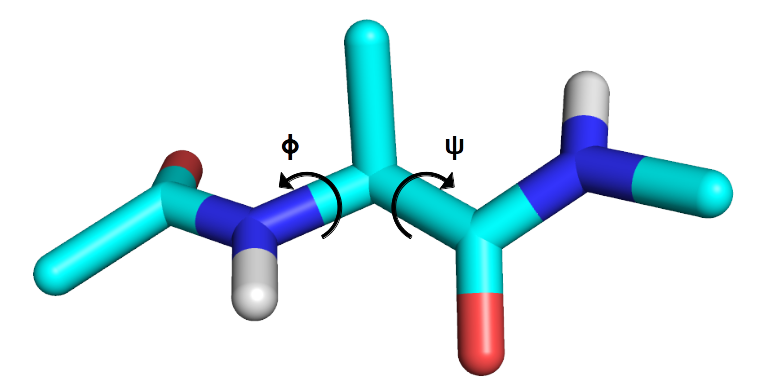
\includegraphics[scale=.3]{../07_tutorial_04/figures/aladip}
\caption{Stick representation of alanine dipeptide with the $\phi$ and $\psi$ dihedrals highlighted.}
\label{aladip}
\end{figure}
 
The preparation of the topology, coordinates, the energy minimization and the equilibration of the system follow the same procedure as described in tutorial 1.
The final equilibrated structure can be found in the directory \texttt{eq} with the name \texttt{aladip\_equilibrated.cnf}.

\subsubsection{GaMD regions definition}
The first step to perform GaMD simulations is to create a GaMD input file containing all the information of which groups of interactions to accelerate and how they need to be accelerated. 
On the directory \texttt{gamd\_setup}, you will find two files, one with the definitions to run standard GaMD, \texttt{ala.gamd}, and one showcasing the selective GaMD functionality, \texttt{selective\_ala.gamd}. Take a look to the block \texttt{GAMDATOMS} of both files.
\begin{lstlisting}
# Standard GaMD:
-----------------------------
GAMDATOMS
1
#  INATOM   FINATOM   AGROUP      
        1      3840        1
END
------------------------------
# Selective GaMD:
------------------------------
GAMDATOMS
2
#  INATOM   FINATOM   AGROUP      
        1        12       1
       13      3840       2
END
------------------------------
\end{lstlisting}
With \texttt{GAMDATOMS} you specify the number of groups of atoms to account for separately. The next line indicates the index of the first atom of the group, \texttt{INATOM}, the final atom, \texttt{FINATOM}, and an integer that will be assigned to that group, \texttt{AGROUP}, (groups of atoms with the same \texttt{AGROUP} index will be considered a single group). In the case of standard GaMD, only one set of atoms is defined. For selective GaMD, the user can define as many atom groups as desired. In the case of this tutorial, two atom groups are defined, one containing the solute (\texttt{AGROUP} = 1), and one containing the solvent (\texttt{AGROUP} = 2).
Now take a look at the second block of the \texttt{.gamd} files.
\begin{lstlisting}
# Standard GaMD:
-----------------------------
GAMDGROUPS
1
# AGROUP_1   AGROUP_2   ACCELGROUP
  1          1          1
END
------------------------------
# Selective GaMD:
------------------------------
GAMDGROUPS
1
# AGROUP_1   AGROUP_2    ACCELGROUP
  1          1           1
  1          2           1
END
------------------------------
\end{lstlisting}
This block defines the number of acceleration potentials to use, and to which interactions they should be applied.
In a similar fashion as with the previous block, \texttt{GAMDGROUPS} specifies the number of distinct acceleration potentials to use. 
The next lines assigns each group of interactions to their corresponding acceleration group were \texttt{AGROUP\_1} and \texttt{AGROUP\_2}  are the indexes of the atom groups defined in the previous block and \texttt{ACCELGROUP} is the index for the acceleration potential. 
In the case of standard GaMD, we have only one acceleration group containing the interactions of all the atoms of the system. For the selective GaMD, the interactions of the alanine didpeptide with itself (\texttt{AGROUP\_1} = 1, \texttt{AGROUP\_2} = 1) and the interactions of the alanine dipeptide with the solvent (\texttt{AGROUP\_1} = 1, \texttt{AGROUP\_2} = 2) are assigned to one acceleration group. The interactions of the solvent with itself (\texttt{AGROUP\_1} = 2, \texttt{AGROUP\_2} = 2) are not assigned to any group and thus not accelerated. The same behaviour can be obtained by using \texttt{ACCELGROUP} = 0, which is never accelerated.

\subsubsection{Acceleration parameter search}
In order to get the acceleration parameters (E and K) a search simulation needs to be performed. The search starts with a conventional MD (cMD) simulation in which the necessary statistics are recorded. After the cMD search, a starting set of $E$ and $K$ parameters is computed and applied to the system. After an equilibration phase, the statistics are collected again and the acceleration parameters are constantly updated. After the adaptive GaMD search, the final acceleration parameters are collected to be used for the production simulations. In this tutorial we will use 0.1 ns of cMD search followed by 0.3 ns of GaMD search. For a real case scenario the search phase must be run for longer times, at least 10 times longer than the searches described here.
Go to the directory \texttt{search}, in there you will find two directories, one for the search of the standard GaMD methodology \texttt{gamd}, and one for the selective approach \texttt{selective\_gamd}. Take a look at the \texttt{GAMD} block of the input file.
\begin{lstlisting}
GAMD
  1
# SEARCH  FORM  THRESH  NTIGAMDS
       1     1       1        1
# AGROUPS  IGROUPS
       1    1
# DIHSTD  TOTSTD
  24.79   24.79
#ED
  0
#ET
  0
#KD
  0
#KT
  0
#EQSTEPS
  0
#WINDOW
  0
END
\end{lstlisting}
The fourth line specifies the general parameters for the GaMD simulation, such as the search algorithm to use (\texttt{SEARCH}), whether the dihedral term has to be accelerated by separate (\texttt{FORM}), whether the energy threshold used is an upper or lower bound (\texttt{THRESH}), and whether the search needs to be initialized (\texttt{NTIGAMDS}). For this tutorial we will accelerate dihedral and potential term by separate (dual boosting approach) and the energy threshold will be set at the lower bound ($E$ = $V_{max}$). 
The next line contains the number of atom groups and interaction groups or acceleration groups defined in the gamd file.
\texttt{DIHSTD} and \texttt{TOTSTD} correspond to the values of $\sigma_0$ for the dihedral term boosting and the potential term boosting respectively.  
The variables $ED$, $ET$, $KD$ and $KT$ are the acceleration parameters that define the boosting potential that will be applied to the system. $ED$ and $ET$ correspond to the list of energy thresholds for the dihedral terms and the potential energy of the system respectively, while $KD$ and $KT$ correspond to the list of force constants of the boosting potential applied to the dihedral term and to the potential energy term. Since this is a search run, all the parameters can be set to 0, for a production run, this parameters will need to be updated for the ones found during the search. Since each acceleration region requires its own parameters, if more than one acceleration region is defined, one must provide extra $ED$, $ET$, $KD$ and $KT$ parameters.
Finally, \texttt{EQSTEPS}  correspond to the number of equilibration steps to use before starting to collect statistics of the search simulation and \texttt{WINDOW} is the size of the window to use to collect the parameters, when \texttt{WINDOW} equals 0 the whole simulation is used to compute the needed statistics.

All input files are now prepared and we can generate the run file with:
\begin{lstlisting}
$ mk_script @f mkscript_gamd_search.arg
\end{lstlisting}
The job file \texttt{gamd\_search.jobs} provided to mk\_script shows the parameters that change between search runs.

For this tutorial we provide two mk\_script libraries, one to prepare the run files for a cluster using SLURM as a queueing system (\texttt{libs\/mkscript.lib}), and one for running the simulations locally, (\texttt{libs\/mkscript\_local.lib}). If the CUDA acceleration code is to be used, one simply needs to uncomment the block \texttt{INNERLOOP} from the imd files before running mk\_script.

After running the GaMD simulation, we can extract the acceleration parameters by using \texttt{ene\_ana}. The analysis files are provided in the folder \texttt{ana}.
We will use this program to read out the energy thresholds and force constants from the last energy trajectory.

You can run the program with 
\begin{lstlisting}
$ ene_ana @f ene_ana.arg
\end{lstlisting}

The file \texttt{ene\_ana.arg} contains the information of which parameters to extract from the energy trajectory. The definitions of those parameters can be found on the library file \texttt{ene\_ana.md++.lib}. This program will generate the trajectories of the selected parameters. The name of the parameters use the following syntax, "gamd\_" (to indicate that is a gamd parameter), followed by parameter to extract (in lower case), followed by the number of the acceleration region. For example, the energy threshold for the dihedrals ($ED$) for the first acceleration group, will be \texttt{gamd\_ed1}.

\subsubsection{GaMD production run}
Now that the search is complete we can run the production run.
Go to the directory \texttt{prod}. In a similar fashion to the \texttt{search} directory, there you will find two directories, one for the standard GaMD methodology \texttt{gamd}, and one for the selective approach \texttt{selective\_gamd}. 
The same imd used in the search runs can be used for the production ones. However, the search algorithm needs to be turned off (\texttt{SEARCH} = 0) and the acceleration parameters obtained from the search run need to be added in. 
For this tutorial, since the search run was not long enough to obtained optimal acceleration parameters, the imd files already contain all the acceleration parameters needed in them, estimated from a longer GaMD search. We will run a production simulation for a total of 1ns, although a true production run must be much longer.

The run files can be created in the same way as in the search runs by using mk\_script with its corresponding .arg file.

\subsubsection{GaMD analysis}

All the analyses for the GaMD simulations will be performed in the subfolder \texttt{ana}. 
In this section of the tutorial we will calculate the reweighted PMF for the $\phi$ and $\psi$ dihedrals of the alanine dipeptide. The same procedure can be used with any other collective variable of interest.
To extract the dihedral angle time series, first we need to run the program \textt{tser} with the correct argument files. You will find two argument files in the folder, on for each dihedral of interest, eg: \texttt{phi\_dihedral\_tser.arg}.
 \begin{lstlisting}
$ tser @f phi_dihedral_tser.arg > phi.out
\end{lstlisting}

The argument files already contain the information needed to compute the dihedrals over time accounting for periodicity, providing values from -180 to 180 degrees.
The next step is to extract the trajectory of the biasing potential used to then be able to reweight the obtained dihedral time series. This can be achieved by using the program \texttt{ene\_ana} in a similar fashion to how the acceleration parameters from the search were extracted. The values of interest are \texttt{totgamd\_dV} which contains the total boosting potential in kJ\/mol, \texttt{totunbiased} which contains the total potential energy excluding the boosting potential and \texttt{totpot} which contains the total potential energy. The boosting potential for each acceleration region can also be extracted independently by adding \texttt{gamd\_dVi} to the ene\_ana property list  @prop with the \texttt{i} sub-index indicating the acceleration group of interest.
After obtaining the collective variables (CV) and biasing potential trajectories, the next step is to reweight and plot them. We will do this using both exponential reweighting and cumulant expansion to the second order.
In the exponential reweighting, the time series of observed values of X (in this case the dihedral angles) sampled during the biased simulation R can be reweighted to the unbiased state Y using the following equation:

\begin{equation}
  \begin{aligned}
 \langle X \rangle_Y = \frac {\langle X \exp \left[-\beta \left (V_Y - V_R \right) \right] \rangle_R} {\langle \exp \left[-\beta \left (V_Y - V_R \right) \right] \rangle_R} = \langle X \exp \left[-\beta \left (V_Y - V_R -\Delta F_{YR} \right) \right] \rangle_R
\end{aligned}
\end{equation}
where $\Delta F_{YR} = F_{Y} - F_{R}$.

The gromos toolkit offers a program called \texttt{reweight} that can be used to reweight time series of observed properties and produce a histogram of the selected number of bins. During the reweightening process special care is taken in order to avoid overflow \cite{berg2003multicanonical}. A sample input file is provided under the name of \texttt{reweight.arg}. Note that the reweight program only accepts a single time series at a time. The script \texttt{ExponentialReweighing.py} provided in the \texttt{scripts} folder can be used to reweigh the probability distribution of interest $p_{R}(\phi, \psi)$. \texttt{ExponentialReweighing.py} first discretizes the two dimensional dihedral angle matrix into a one dimensional time series. The probability distribution of this time series is then computed and reweighted using the \texttt{reweight} program. Finally, the one dimensional reweighted probability distribution is mapped back to a two dimensional probability distribution, $p_{Y}(\phi, \psi)$, and converted to energies to be able to plot them.
 \begin{lstlisting}
$ python ExponentialReweighing.py --cv1 phi.out --cv2 psi.out --vr totpot.dat --vy totunbiased.dat --xdim -180 180 10 --ydim -180 180 10
\end{lstlisting}

An alternative way of reweighting the trajectories would be to use cumulant expansion to the second order to approximate the reweighting factor. The reweighted free energy  $F_{Y}(\phi, \psi)$ will then be calculated as:
\begin{equation}
  \begin{aligned}
 F_{Y}(\phi, \psi) = F_{R}(\phi, \psi) - \sum_{k=1}^{2} \frac{\beta^{k}}{k!}C_{k} + F_{c}
\end{aligned}
\end{equation}
where $F_{c}$ is a constant, $F_{R}(\phi, \psi)$ is the free energy obtained from the unreweighted trajectory, $F_{R}(\phi, \psi) = -k_{B}T \ln{p_{R}(\phi, \psi)}$ and the first two cumulants are:
\begin{equation}
  \begin{aligned}
C_{1} = \langle \Delta V \rangle,\\
C_{2} = \langle \Delta V^2 \rangle - \langle \Delta V \rangle^2 = \sigma^{2}_{v}
\end{aligned}
\end{equation}
This can be achieved by using the pyreweight script that is provided in the \textttt{scripts} directory or that can be downloaded from its original repository \cite{miao2014improved}.

The version provided in the \textttt{scripts} folder contains a small modification to provide the results in kJ/mol to ease the comparison to the results provided by GROMOS. The script takes as input a file with the CVs in columns and another file with the biasing potential with three columns, biasing in kJ/mol, time, and biasing in kcal/mol. An example of how to run the script can be found on the \textttt{scripts} folder on the file \textttt{pyreweight\_command.txt}.

Because the performed trajectories are too short to obtain converged PMFs, the dihedral and energy trajectories of a 100 ns run are provided in the subfolder \texttt{data}. The same analysis can be performed on the files provided there, producing the 2D-PMFs in figure \ref{aladip_pmf}:

\begin{figure}[H]
\centering
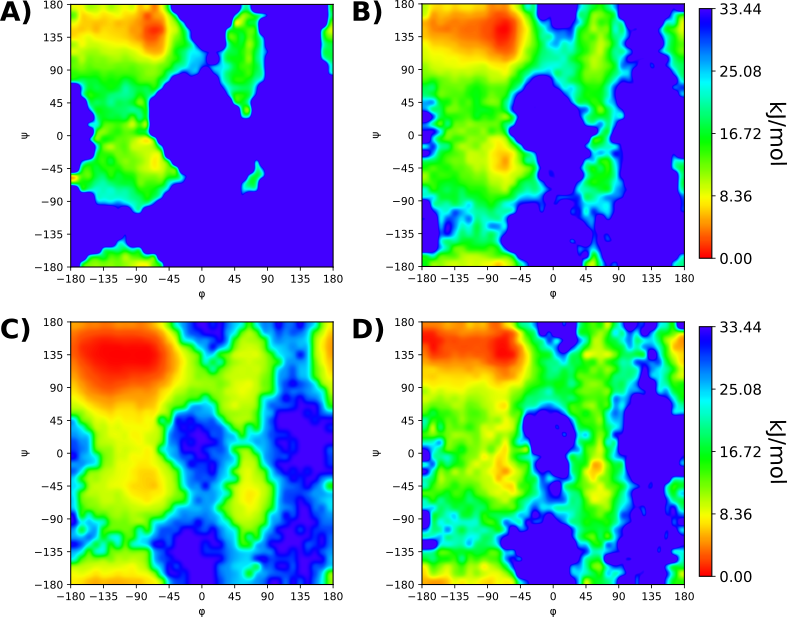
\includegraphics[scale=.43]{../07_tutorial_04/figures/pmf_tutorial}
\caption{Potential of Mean Force (PMF) profiles over the $\phi$ and $\psi$ angles of the alanine dipeptide. A) Simulation using the standard GaMD approach reweighted with cumulant expansion to the second order. B) Simulation using the standard GaMD approach reweighted with exponential reweighing. C) Simulation using the selective GaMD approach reweighted with cumulant expansion to the second order. D) Simulation using the selective GaMD approach reweighted with exponential reweighing. }
\label{aladip_pmf}
\end{figure}




% Tutorial 05

\subsection{Tutorial 5: Accelerated Enveloping Distribution Sampling (AEDS)}

Alchemical free-energy methods have been established as an irreplaceable tool in computational drug design. A vast variety of methods to perform alchemical transformations exists. We have already seen the extended-Ti approach outlined in section \ref{chapt:exTI}. One family of free-energy methods is the free-energy perturbation (FEP) based on Zwanzig´s equation (eq. \ref{eq:Zwanzig1}) \cite{Zwanzig1954}. Defining the free-energy difference $\Delta G_{i,j}$ between two states $i$ and $j$, represented by Hamiltonian's $H_i$ and $H_j$ over the positions $\vec{r}$ as an ensemble average over state $i$. 

\begin{equation}
\begin{aligned}
\Delta G_{i,j} & = G_j - G_i \\ & = -k_BT \ln  \Biggl \langle e^{ -(H_j(\vec{r}) - H_i(\vec{r}))/k_BT} \biggr \rangle_i 
\end{aligned}
\label{eq:Zwanzig1}
\end{equation}

As mentioned in section \ref{chap:tut2} sampling relevant phase-space is of utmost importance to converge to plausible results. While methods like TI \cite{kirkwood_TI} or BAR \cite{bar} aim to connect physical states through non-physical states, one-step perturbation methods take a different approach. Here, a reference Hamiltonian, constructed from the end-states, is sampled. This avoids spending simulation time on non-relevant states. This method fits perfectly to investigate closely related systems like derivates. In this tutorial, we will take a look at accelerated enveloping distribution sampling (AEDS) \cite{JP2018,JP2020}. In enveloping distribution sampling a reference Hamiltonian $H_R(\vec{r})$ is constructed by combining several different end-state Hamiltonian's $H_i(\vec{r})$. To achieve equal sampling of each of the end-states, $H_i(\vec{r})$ is biased by an offset $\Delta F_{i}^R$. The partition function of $H_R(\vec{r})$ results now as the sum of the biased end-state partition functions (eq. \ref{eq:EDS1}).
%\nameref{equ:ext_ti}
\begin{equation}
\begin{aligned}
H_R(\vec{r}) & = -k_BT \ln  \left( \sum_{i=1}^{N} e^{ -(H_i(\vec{r}) - \Delta F_{i}^R)/k_BT} \right) 
\end{aligned}
\label{eq:EDS1}
\end{equation}

Since this approach can lead to high energy barriers between the minima and thus to sampling problems, the original EDS version introduced a smoothing parameter $s$ (eq. \ref{eq:EDS2}) to smoothen the energy landscape. 

\begin{equation}
\begin{aligned}
H_R(\vec{r}) & = -\frac{k_BT}{s} \ln  \left( \sum_{i=1}^{N} e^{ -s(H_i(\vec{r}) - \Delta F_{i}^R)/k_BT} \right) 
\end{aligned}
\label{eq:EDS2}
\end{equation}

This can lead to a deformation of the energy landscape, not preserving the position of the energy minima. Therefore, a refined approach using a boosting potential was proposed \cite{JP2018,JP2020}. Similar to Gaussian accelerated MD, a harmonic boosting potential is used to accelerate defined regions, namely the non-bonded interactions of the perturbed atoms. The accelerated reference Hamiltonian $H_R^{\ast}(\vec{r})$ is defined as shown in equation \ref{eq:AEDS}, where the acceleration range is defined by $E_{max}$ and $E_{min}$. 

\begin{equation}
  \begin{aligned}
H_R^{\ast}(\vec{r}) =\begin{cases}
        H_R(\vec{r}) - \frac{E_{max} - E_{min}}{2} &\text{if} \, H_R(\vec{r}) \geq E_{max} \\

        H_R(\vec{r}) - \frac{1}{2(E_{max} - E_{min})}(H_R(\vec{r}) -  E_{min})^2 &\text{if} \,  E_{min} < H_R(\vec{r}) < E_{max} \\

        H_R(\vec{r}) &\text{if} \, H_R(\vec{r}) \leq E_{min} \\
     \end{cases}
  \end{aligned}
  \label{eq:AEDS}
\end{equation}

To obtain parameters for $E_{max}$, $E_{min}$, and the offsets a parameter search simulation is necessary. In the search simulation, the currently sampled state is defined as the state with the lowest energy for $H_i(\vec{r}) - \Delta F_{i}^R$. $E_{max}$ is defined as the maximum observed transition energy after a full state round trip, meaning that each state was sampled at least once. $E_{min}$ is based on the fluctuations of $H_i(\vec{r})$ of the state with the lowest energy. The offsets have different definitions depending on the search algorithm in use. Generally, the difference between two offsets $\Delta\Delta F_{ij}$ is the free-energy difference between the accelerated end-states $i$ and $j$. In older iterations of the search algorithm, the offsets were estimated as the free-energy difference between an accelerated end-state and the accelerated reference state and afterward anchored to one of the end-states. The search algorithm used in this tutorial uses an approach similar to local elevation by continuously adding to the offsets based on their sampling probability. In this approach, all offsets are averaged around zero. This has proven to be a more robust search algorithm and removed the dependency on the anchor state. The parameters obtained from the search simulation are then used in a production run.

\subsubsection{Preparations}
In this tutorial, we will use two SPC water molecules as a test system. We will use AEDS to calculate free-energy differences and as a tool for water probing in a protein-ligand system \cite{gracia1}.   
 
The preparation of the topology, coordinates, energy minimization, and equilibration of the system follows the same procedure as described in tutorial 1.
The final equilibrated structures can be found in the directory \texttt{eq}. The perturbation topologies can be created as shown in tutorial 2 and are provided in the directory \texttt{topo}.

\subsubsection{Acceleration parameter search}
To get the acceleration parameters ($E_{max}$, $E_{min}$, offsets) a search simulation needs to be performed. The search run starts from an equilibrated structure. If no initial parameters are given the search starts as a conventional MD simulation. After each simulation step $E_{max}$, $E_{min}$, and the offsets are updated. After approximately 5-25 ns the parameter search simulation converges. The needed simulation time depends mostly on the complexity of the system and the perturbation since we are dependent on visiting all end-states to adjust the acceleration parameters. In this tutorial, we will run a very short search simulation of 0.5 ns and use parameters from a longer simulation for the production run.  

Go to the directory \texttt{search}. In this folder, you will find three files namely \texttt{aeds.arg}, \texttt{aeds.job}, and \texttt{aeds.imd}. Let's start with the \texttt{aeds.imd} file. This file is a simulation input file we already know from previous tutorials. At the bottom of the file, we have an additional \texttt{AEDS} block.
\begin{lstlisting}
AEDS
# AEDS
     1
# FORM  NUMSTATES
     5          4
# EMAX  EMIN
     0     0
# EIR [1..NUMSTATES]
    0   0   0   0 
# NTIAEDSS  RESTREMIN   BMAXTYPE    BMAX 
         1          1         2        2    
# ASTEPS    BSTEPS
    1000     10000 
END
\end{lstlisting}
In the second line, we set $FORM$ to 5 specifying an all-parameter search using the adaptive search.
Later we will change this into $FORM$ 1 to run a production run. Other options are described in the  \texttt{gromos} handbook. $NUMSTATES$ specifies the number of end-states in this simulation. Since we perturb two SPC water molecules A and B we get four possible end-states as all combinations of A and B being present or dummies as shown in table \ref{tab:states}.

\begin{table}[h!]
    \begin{center}
     \begin{tabular}{*{3}{m{0.1\textwidth}}}
      & \hfil A & \hfil B \\
       \toprule
        end-state 1
      & 
        \begin{center}
\includegraphics[width=0.08\textwidth]{../08_tutorial_05/figures/water.png}\end{center}
      & 
        \begin{center}
\includegraphics[width=0.08\textwidth]{../08_tutorial_05/figures/water.png}\end{center} \\
        end-state 2
      & 
        \begin{center}
\includegraphics[width=0.08\textwidth]{../08_tutorial_05/figures/dummy.png}\end{center}
      & 
        \begin{center}
\includegraphics[width=0.08\textwidth]{../08_tutorial_05/figures/dummy.png}\end{center} \\
        end-state 3
      & 
        \begin{center}
\includegraphics[width=0.08\textwidth]{../08_tutorial_05/figures/water.png}\end{center}
      & 
        \begin{center}
\includegraphics[width=0.08\textwidth]{../08_tutorial_05/figures/dummy.png}\end{center} \\
        end-state 4
      & 
        \begin{center}
\includegraphics[width=0.08\textwidth]{../08_tutorial_05/figures/dummy.png}\end{center}
      & 
        \begin{center}
\includegraphics[width=0.08\textwidth]{../08_tutorial_05/figures/water.png}\end{center} \\
      \bottomrule
      \end{tabular}
      \caption{Showing the resulting end-states 1-4 for the perturbation of two SPC water molecules A and B.}
      \label{tab:states}
    \end{center}
\end{table}

In the third line, we set zeros for both $E_{max}$ and $E_{min}$ as well as for the offsets in the line underneath. If we had prior information about these values we could give them as a starting point for the search instead of starting from scratch. Line five is specific for search runs. With $NTIAEDSS$ 1 we initialise the search run. You will see that we turn it off in the jobscript after the first initialization. $RESTREMIN$ restricts $E_{min}$ to the minimum average end-state energy before all states have been visited at least once. $BMAXTYPE$ and $BMAX$ are used to control the estimated maximum barrier height. By default, we set both of them to 2. $ASTEPS$ is used to control the change rate in offsets. A higher number means a faster change in offsets. $BSTEPS$ is used for initial free-energy guesses in other search algorithms. In the argument file, we need to specify the folder location and the location of the md binaries as absolute paths. The \texttt{imd} file uses the $INNERLOOP$ block for \texttt{CUDA} support. If the used \texttt{gromos} binary does not support \texttt{CUDA}, comment the block out using hashtags. The jobfile is used to create ten \texttt{imd} and \texttt{run} files of the same simulation length as specified in \texttt{aeds.imd}. The only changes in the settings are that 
$NTIAEDSS$ is set to zero after the first jobscript.

With all input files prepared, we can now generate the run files using \texttt{mk\_script} from \texttt{gromos++} package with:
\begin{lstlisting}
$ mk_script @f aeds.arg
\end{lstlisting}

For this tutorial, we provide two \texttt{mk\_script} libraries, one to prepare the run files for a cluster using SLURM as a queueing system (\texttt{libs/mk\_script.lib}), and one for running the simulations locally, (\texttt{libs/mk\_script\_local.lib}).

After running the parameter search simulation, we can extract the acceleration parameters by using \texttt{ene\_ana}. The analysis files are provided in the subfolder \texttt{ana} in the search directory. 
We will use this program to read out the energy and offset of each end-state as well as $E_{max}$ and $E_{min}$. 

You can run the program with 
\begin{lstlisting}
$ ene_ana @f ene_ana.arg
\end{lstlisting}

The file \texttt{ene\_ana.arg} contains the information of which parameters to extract from the defined energy trajectories. The definitions of those parameters can be found in the library file \texttt{libs/ene\_ana.md++.lib}. \texttt{ene\_ana} will generate trajectories of the selected parameters. We could plot \texttt{eds\_emin.dat}, \texttt{eds\_emax.dat}, and \texttt{e*r.dat} to check for convergence, where the * in \texttt{e*r.dat} is to be replaced by the end-state number. These files contain the offsets for each end-state. Another way is to use \texttt{search.py} in the scripts folder. This script splits the trajectories into ten blocks and gives us the average $E_{min}$ and $E_{max}$ of the last block in the first line. Underneath the offsets with an error estimate for each end-state averaged for each block are shown. It also calculates the theoretical offsets, as the free-energy difference to the accelerated reference state, shown in the third column. In an ideal case, the offset values converge to a single value in the later blocks and have a small error estimate. In addition, they should be similar to the theoretical offset meaning the free-energy difference between the accelerated end-state and the accelerated reference state. Keep in mind that the offsets in column one are averaged around zero.
To call \texttt{search.py} in the \texttt{search/ana} folder, do the following:

\begin{lstlisting}
$ python ../../scripts/search.py
\end{lstlisting}

The output from the longer search run can be found in \texttt{search/ana/long}.
We will use $E_{min}$ and $E_{max}$ as well as the offset parameters from the last block of each end-state found in \texttt{search.out}.

\subsubsection{AEDS production run}
With the parameters from the search run, we can now start a production run. From the production run, we can calculate our relative free energies. Go into the directory \texttt{prod}. Here we see two files, \texttt{aeds.arg} and \texttt{aeds.imd}. We do not use the $@joblist$ argument in the argument file, but the $@script$ argument to specify the number of jobs. If we take a short look into \texttt{aeds.imd} we will spot a few differences:

\begin{lstlisting}
AEDS
# AEDS
     1
# FORM  NUMSTATES
     1          4
# EMAX  EMIN
    43.08  -187.95
# EIR [1..NUMSTATES]
 16.32   -43.66   12.99    14.35 
# NTIAEDSS  RESTREMIN   BMAXTYPE    BMAX   
         0          1         2        2      
# ASTEPS    BSTEPS
    1000     10000 
END
\end{lstlisting}

We now use $FORM$ 1 for a production run. We also inserted values for $E_{max}$, $E_{min}$, and the offsets. We also set $NTIAEDSS$ to zero which is optional since this line is not read in a production run. Similar to the search run we now use \texttt{mk\_script} to create our input files. Again, the $INNERLOOP$ block in the \texttt{imd} file has to be commented out if the used \texttt{gromos} binary does not support \texttt{CUDA}.
Since we use well converged parameters we can get away with a short production run of 1 ns. In practice, production runs are mostly between 20-100 ns.

\subsubsection{Production run analysis}
The analysis will be done in the subfolder \texttt{prod/ana}. We will do two kinds of analysis. Firstly, we will take a look at the free-energy difference between the end-states using \texttt{ene\_ana} and \texttt{dfmult}. Secondly, we will take a look into the fractional occupancy of the end-states. We will use this information in the water probing section later on. All values shown are from a longer production run. The files can be found in the subfolder \texttt{prod/ana/long}. To start with analysis we will run the following commands:

\begin{lstlisting}
$ ene_ana @f ene_ana.arg
\end{lstlisting}

and after that we use

\begin{lstlisting}
$ dfmult @f df.arg > df.out
\end{lstlisting}

\texttt{ene\_ana} generates the trajectories of the selected parameters as before. We use \texttt{dfmult} to calculate free energies and save them in \texttt{df.out}. If we take a look at the \texttt{df.out} file we will see the following:

\begin{lstlisting}
            #DF (kJ/mol)               err
DF_1_R     2.1428295e+01     6.9032914e-02
DF_2_1     5.3410399e+01     7.9494696e-02
DF_3_1     2.5792504e+01     3.0323318e-01
DF_4_1     2.6096480e+01     1.9175297e-01
DF_2_R     7.4838694e+01     3.8460413e-02
DF_3_2    -2.7617895e+01     2.9776361e-01
DF_4_2    -2.7313919e+01     1.8298067e-01
DF_3_R     4.7220799e+01     2.9514515e-01
DF_4_3     3.0397569e-01     3.4513025e-01
DF_4_R     4.7524775e+01     1.7868847e-01
\end{lstlisting}

In each row, we see a specifier like $DF\_1\_R$ meaning end-state 1 to the reference state, the relative free energy in kJ/mol, and an error estimate in kJ/mol. From two water present to no water present we get a free-energy difference of $53.3 \pm 0.1$ kJ/mol. From two water to one present and one not present we get $25.9 \pm 0.3$ kJ/mol and $26.2 \pm 0.3$ kJ/mol. Turning two different single water into dummies produces free energies in good agreement with each other as well as doing two at the same time which is roughly double the solvation free energy of a single water molecule. The values also agree with values from the literature \cite{gracia1}. To estimate the quality of our free energies as well as to estimate the time of occupancy for each end-state we use the \texttt{prevalence.py} script like:

\begin{lstlisting}
$ python ../../scripts/prevalence.py
\end{lstlisting}

This script gives us an output as follows: 

\begin{lstlisting}
ENDSTATE    WEIGHT      PERCENTAGE  #FRAMES
Endstate 1  53399.95    26.7        37491
Endstate 2  52681.49    26.34       58881
Endstate 3  42163.19    21.08       5621
Endstate 4  50356.36    25.88       7325
\end{lstlisting}

Showing the accumulated probability of each end-state over all frames (WEIGHT), the same value in percentage (PERCENTAGE), and the total number of frames that contributed to the final free energy within a cutoff of one $k_BT$ (\#FRAMES). The more frames contribute to the free energy the more certain we are to sample the true minimum of that state. Free energy estimates based on just a few frames are less trustworthy. If we use too much acceleration, this leads to a very flat energy surfaces, and we struggle to sample the real minima. In such a case, one would still find a lowest energy for that end-state which do not necessarily represent the true minimum, since the information was lost due to the flattening of the energy surface. 
As you can see the parameters used resulted in a roughly equal sampling of all of the end-states. This means that we converged to values that result in an equilibrium between our end-states during the production run. Endstate 3 is slighty underrepresented in comparison and one could try to refine the parameter set to get more equal sampling. We will use this set of parameters in the water probing to catch the influence of a change in the environment on the sampling times.

\subsubsection{Water probing}
To capture the influence the environment has on our sampled water, we set up a production run with the parameter set optimized for the water environment in a protein-ligand environment. The Woodhead-2 system (pdb:2XJG\cite{woodhead2}) is used in this tutorial. Go into the folder \texttt{water\_probing}. Similar to the production run in water we have two files, \texttt{aeds.arg} and \texttt{aeds.imd} in the directory. Looking into \texttt{aeds.arg} we will see a few changes. Besides using the topology and coordinates for the Woodhead-2 system we also use a different perturbation topology since the perturbation file depends on the atom number in the topology which is changed because we now have a protein in our system. Additionally, we are also using distance restraints on the water molecules. The reason being that the end-states with the water turned into dummies have no interactions to keep them in place and the dummies would move out of the binding site. If we now take a look into the \texttt{aeds.imd} file we can see that besides the system-specific changes like the number of atoms, a distance restraint block is added. For more information about distance restraints read Tutorial 2 or check in the in the  \texttt{gromos} handbook. If we take a look at the AEDS block we will see that the same parameters are used as in the production run in water. Since this system is quite large we provide the output files from \texttt{ene\_ana} in the \texttt{water\_probing/ana/long} subdirectory.

After running \texttt{dfmult} and the prevalence script we will get the following:

\begin{lstlisting}
ENDSTATE    WEIGHT      PERCENTAGE  #FRAMES
Endstate 1  3646.0      7.29        3634
Endstate 2  0.06        0.00        23413
Endstate 3  46353.94    92.71       25127
Endstate 4  0.00        0.00        3368
\end{lstlisting}

We see that in the protein environment opposing the production run in water environment, where end-states 1,2,4 were equally likely and end-state 3 a little less likely, that end-state 3 is solely favorable in the protein enviroment, and almost all of the simulation time is spent to sample this state. As we used a parameter set that gives us roughly equal sampling over all end-states in a water environment this shift in sampling is due to the change in environment. This indicates, that just a single water at the position of water A is favored to be present in the binding site.

\subsubsection{Common errors}
\textbf{[Note:} Please document frequently occurring errors, including a clear descriptive title for each error and a brief explanation of how it occurs, how to resolve it, and how to prevent it.\textbf{]}

\paragraph{Error}
cause, indicators, solution, prevention, tips,...



% Tutorial 06

\subsection{Tutorial 6: NN(QM)/MM simulations with the BuRNN approach}
The Buffer Region Neural Network (BuRNN) approach \cite{Lier2022BuRNN} is a hybrid quantum mechanics/molecular mechanics (QM/MM) \cite{Warshel1976QM/MM, Senn2009QM/MM} simulation method. The system is partitioned into regions having different levels of theory, a QM (inner) and a classical MM (outer) region. 

In between the two regions, an additional buffer region is introduced to be treated at both levels of theory (Figure~\ref{BuRNN_scheme}, a). The inner region and the interactions between the inner region and the buffer region are described by an atomistic neural network (NN) model, approximating a QM energy.

The total potential energy of the system is calculated as follows:

\begin{equation}
  \begin{aligned}
  V_{tot} = V^{QM}_{\mathbb{I+B}} - V^{QM}_{\mathbb{B}} + V^{MM}_{\mathbb{B}} + V^{MM}_{\mathbb{O}}
    \end{aligned}
\end{equation}


 The energy difference of the first two terms is then directly described by a neural network potential: 
 
\begin{equation}
  \begin{aligned}
  V_{tot} \cong \mathrm{V}_{\mathbb{I+}\Delta\mathbb{B}}^{NN} + \mathrm{V}_{\mathbb{B+O}}^{MM}
    \end{aligned}
\end{equation}


As a NN model we use SchNet \cite{Schuett2017SchNet, Schuett2018SchNet}, a continuous filter convolutional NN. The deep learning architecture SchNetPack \cite{Schuett2019SPK} is interfaced with the MD engine of GROMOS.



In this tutorial, methanol in water will be used as a model system. In the context of BuRNN, methanol will be the inner region, while water molecules within a radius of 0.5 nm around the methanol will form the buffer region. The remaining water molecules will serve as the outer region. 

We will learn how to install GROMOS with the interface to SchNetPack, generate a training data set, train the NN model and run the BuRNN simulation.


\begin{figure}[H]
\centering
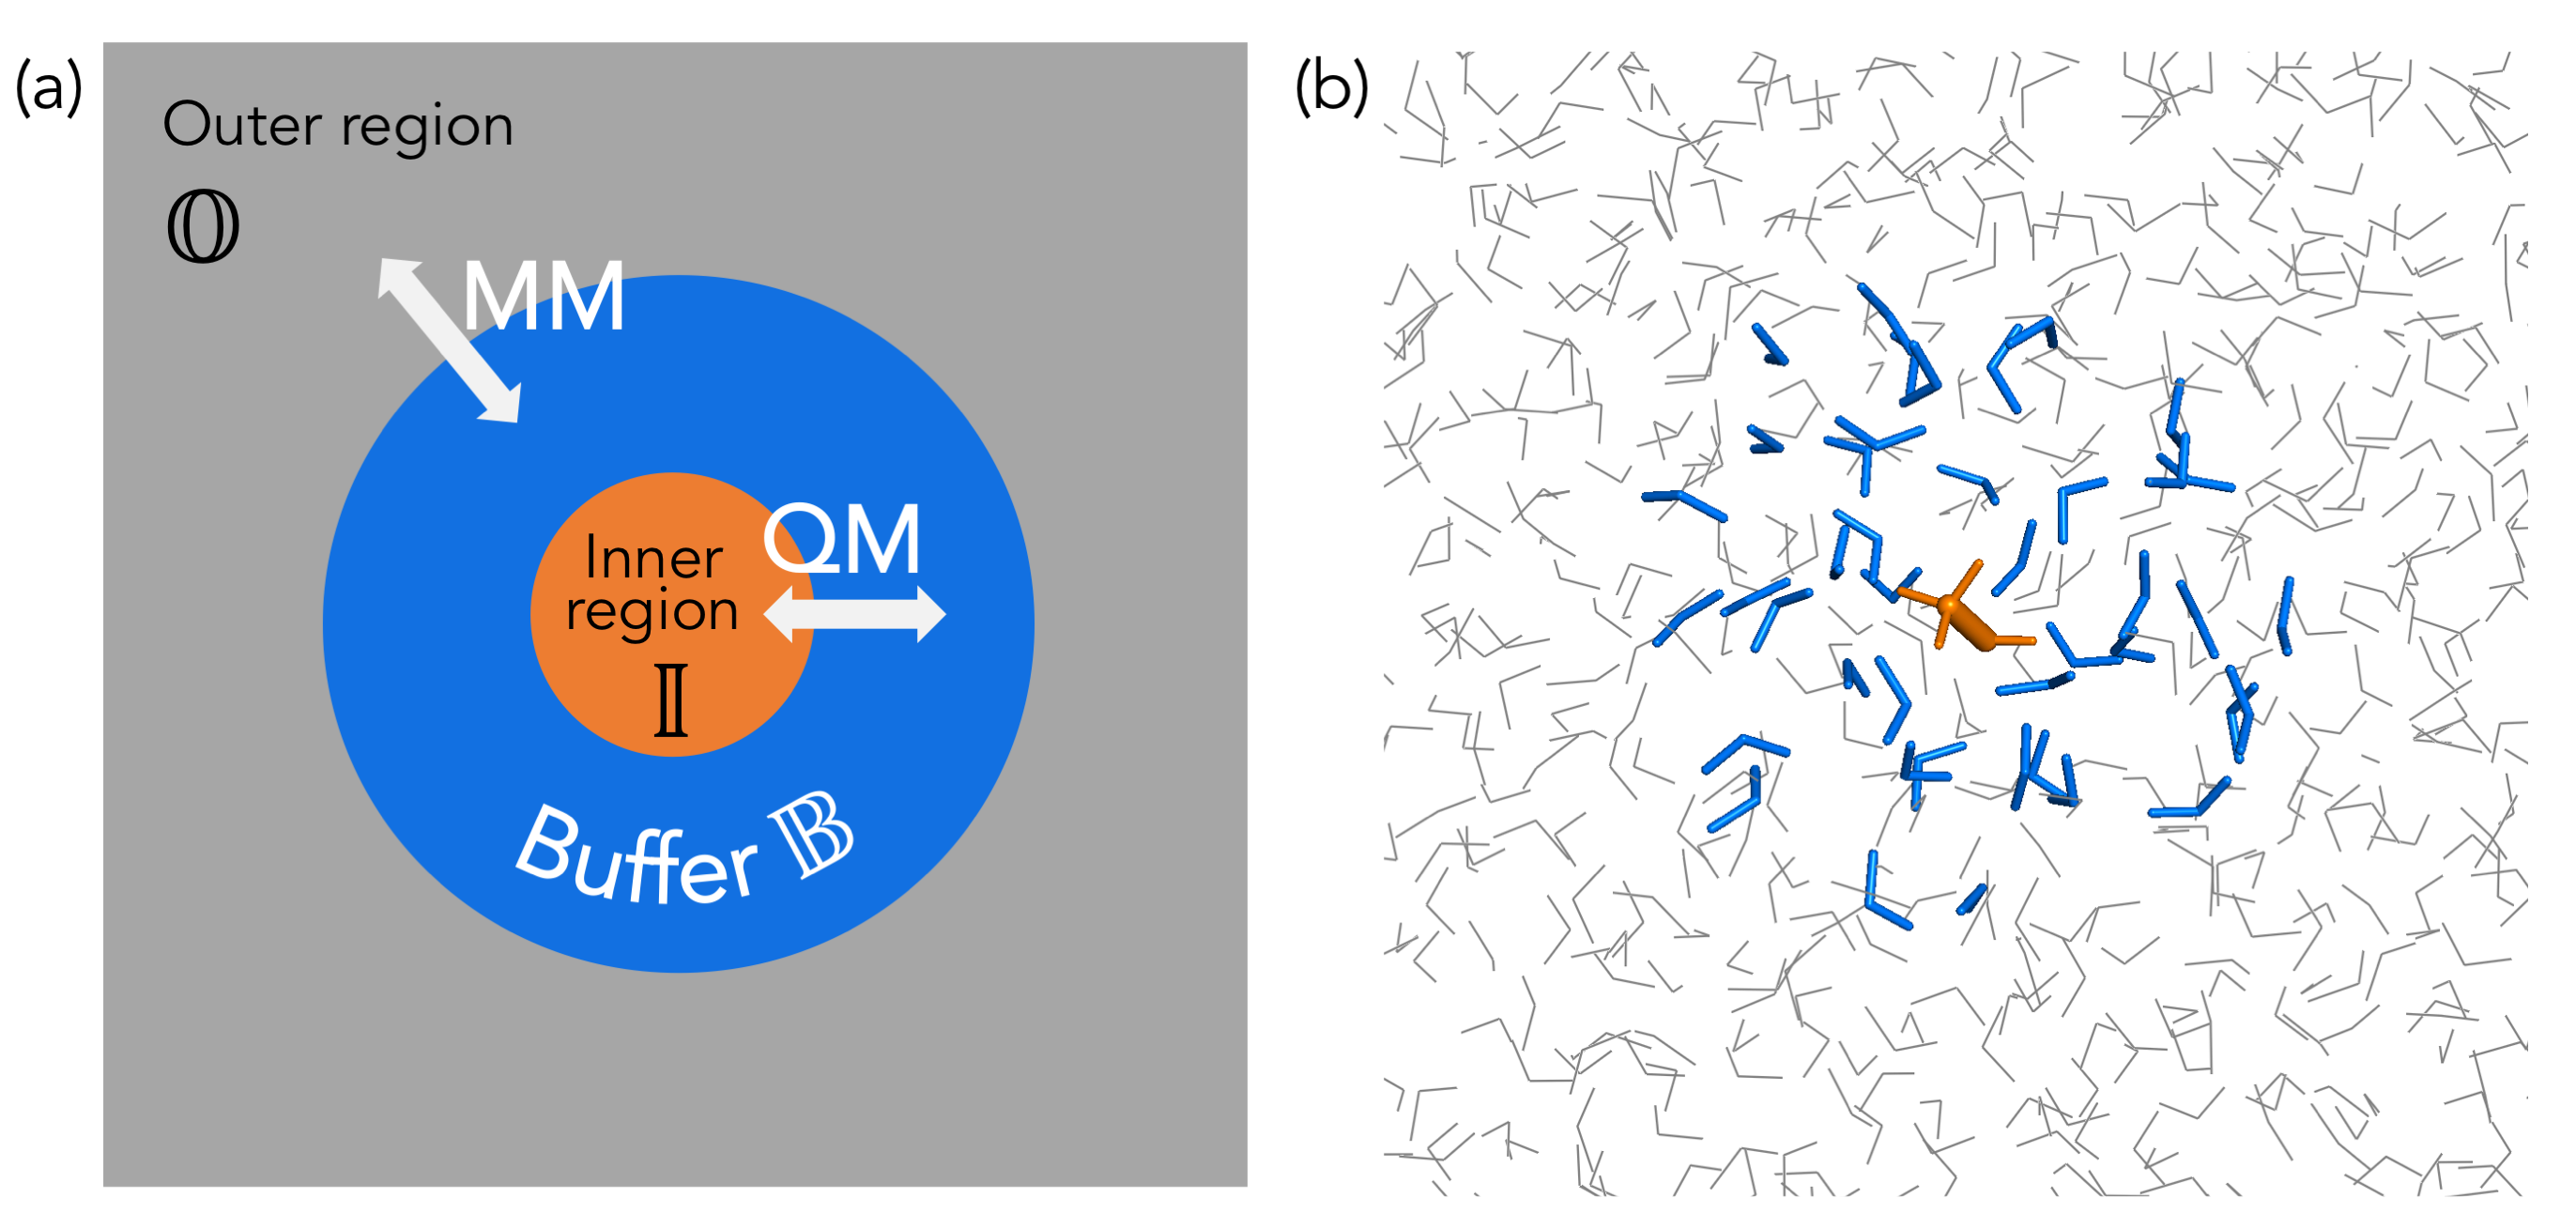
\includegraphics[scale=.33]{../09_tutorial_06/figures/BuRNN_scheme}
\caption{(a) BuRNN scheme with its three regions: Inner region (orange) described by quantum mechanics (QM), buffer region (blue) described by QM and molecular mechanics (MM), outer region (gray) described by MM. (b) Test system: methanol solvated in SPC water. Methanol is the inner region, approximately two shells of water are the buffer region, and the rest of the water box builds the outer region.}
\label{BuRNN_scheme}
\end{figure}


\subsubsection{Installation} \label{chap:burnn_install}
\paragraph{Prerequisites}
To compile and install GROMOS with the interface to SchNetPack (spk) to run NN models, you first need to have installed SchNetPack and the pybind11 library \cite{pybind11}. The interface uses the pybind11 library to call the model prediction functions in the Python code of SchNetPack. To install the SchNetPack and pybind11 library on your system, please follow their respective installation instructions. The tested version of SchNetPack is 1.0.0 and pybind11 v2.6.2.

\paragraph{GPU acceleration}
This part is optional to improve the efficiency of the simulations. The tasks in this tutorial are small enough to be run CPU-only in a reasonable time. For the production runs this is inefficient since the training and evaluation of models on a GPU is usually manifold faster. NN/MM MD simulations in GROMOS profit from this as well. Setting up your system to support the GPU acceleration is strongly architecture specific and is dependent on the installed CUDA and Pytorch versions. Please follow the installation instructions of CUDA and Pytorch to run tasks with the GPU acceleration.

\paragraph{GROMOS compilation}
Compilation of the NN-enabled version of GROMOS is activated by the \texttt{--enable-schnetpack} flag in the configuration step. The \texttt{configure} script looks up the pybind11 library automatically; however, based on the versions of the packages and the architecture, it might not be found. In that case, you should provide the flags \texttt{PYFLAGS} and \texttt{PYLDFLAGS} to the \texttt{configure} script. The \texttt{PYFLAGS} variable holds the C preprocessor flags, which can be obtained by calling

\begin{lstlisting}[breaklines=true, breakatwhitespace=false]
python3 -m pybind11 --includes
\end{lstlisting}

The \texttt{PYLDFLAGS} are the linker flags. Depending on the Python version, they can be generated by calling either 

\begin{lstlisting}[breaklines=true, breakatwhitespace=false]
python3-config --ldflags
\end{lstlisting}

\noindent{for Python version older than 3.8, or} 

\begin{lstlisting}[breaklines=true, breakatwhitespace=false]
python3-config --ldflags --embed
\end{lstlisting}

\noindent{for newer versions. An example of the \texttt{configure} script then could be:}
\begin{lstlisting}[breaklines=true, breakatwhitespace=false, showstringspaces=false]
$ ./configure --enable-schnetpack PYFLAGS='-I/path/to/include/python3.7 -I/path/to/lib/python3.7/site-packages/pybind11/include' PYLDFLAGS='-L/path/to/lib/python3.7/config -L/path/to/lib -lpython3.7 -lcrypt -lpthread -ldl -lutil -lrt -lm'
\end{lstlisting}

Further steps follow the standard compilation:
\begin{lstlisting}[breaklines=true, breakatwhitespace=false]
$ make
$ make install
\end{lstlisting}


\subsubsection{Training dataset generation and model training}
The BuRNN approach replaces expensive QM calculations with NN predictions during MD simulations. In order to train NN models, QM data points for building a training data set have to be generated first. In this tutorial, an example QM data set has been generated using the semi-empirical program MOPAC \cite{Stewart1990MOPAC, Stewart2013MOPAC}. In practice, the choice of the QM software and the reference method to be used is entirely up to the user depending on the system and accuracy requirements. However, in order to prepare the training data set in a reasonable time, it is necessary to automate the QM calculations. In addition, it takes a certain amount of time to perform the QM calculations for all the snapshots generated by MD. Therefore, a small \href{https://github.com/LierB/gromos_tutorial_livecoms/tree/burnn_tutorial_rc/tutorial_files/t_06/train_dataset_tutorial/QM_dataset_example}{QM data set} has been prepared in advance (\texttt{train\_dataset\_tutorial/QM\_dataset\_example}). The initial dataset uses molecular configurations that are generated from a purely classical MD simulation. The entire process is described in the following section.


This tutorial will be accompanied by the \href{https://github.com/LierB/gromos_tutorial_livecoms/blob/burnn_tutorial_rc/tutorial_files/t_06/train_dataset_tutorial/tutorial_v2.ipynb}{jupyter notebook} (\texttt{train\_dataset\_tutorial/tutorial\_v2.ipynb}) to give a hands-on example of building the training database. It will use the in-house written Python module \href{https://github.com/LierB/gromos_tutorial_livecoms/blob/burnn_tutorial_rc/tutorial_files/t_06/train_dataset_tutorial/additional_spk_utils.py}{\texttt{additional\_spk\_utils}} for building the training data set.


\paragraph{Extracting the QM regions from the MD trajectory}
The resulting QM data set will contain the inner plus buffer (IPB) region and the buffer region for each training configuration. Our protocol for creating such a data set is as follows: 
\begin{enumerate}
    \item Classical MD simulation of the system of interest.
    \item Extraction of the IPB regions from the MD trajectory.
    \item QM energy minimization for all (or selected) extracted IPB regions.
    \item Including all configurations along the minimization process into the data set.
    \item Extraction of the buffer regions from all the data points.
    \item Single-Point QM calculations for the IPB and buffer regions separately.
    \item Creation of the training database
\end{enumerate}


Classical MD simulations are performed as described in Tutorial 1. QM regions (inner + buffer regions) are extracted from each snapshot of the MD trajectory using the GROMOS++ program \texttt{filter}. The program writes out coordinate trajectories for atoms that are within a specified distance of a certain part of the system. The coordinates are all written into one \href{https://github.com/LierB/gromos_tutorial_livecoms/blob/burnn_tutorial_rc/tutorial_files/t_06/train_dataset_tutorial/filter/filter_output_example.cnf}{configuration file} (\texttt{filter\_output\_example.cnf}) in the \texttt{train\_dataset\_tutorial/filter} directory.

For methanol, we specify all methanol atoms as filtering centers (\texttt{@atoms 1:a}) and filter with a chargegroup-based cut-off (\texttt{@pairlist CHARGEGROUP}) of 0.5 nm radius (\texttt{@cutoff 0.5}). The optimal/reasonable size for the buffer region can be determined from an rdf analysis. It should be as small as possible, as we want to save computational effort for the following QM calculations. The chargegroup cut-off scheme is important as we want to include full water molecules in the QM calculations. Then we extract individual QM regions into separated configuration files using an in-house written Python script. The arguments we use for \texttt{filter} are as follows:

\begin{lstlisting}[breaklines=true, breakatwhitespace=false]
@topo       <topology file>
@pbc        r cog
@atoms      1:a
@pairlist   CHARGEGROUP
@cutoff     0.5
@outformat  cnf

@traj       <trajectory file(s)>
\end{lstlisting}

We provide an example of two \href{https://github.com/LierB/gromos_tutorial_livecoms/tree/burnn_tutorial_rc/tutorial_files/t_06/train_dataset_tutorial/separated_cnf_files}{configuration files} (\texttt{train\_database\_tutorial/separated\_cnf\_files}) which will be further used in this tutorial. An example of the \href{https://github.com/LierB/gromos_tutorial_livecoms/blob/burnn_tutorial_rc/tutorial_files/t_06/train_dataset_tutorial/filter/filter_meoh_example.arg}{argument file} for \texttt{filter} is provided (\texttt{filter/filter\_meoh\_example.arg}).

\paragraph{QM calculations}
In this part, we mainly focus on the concept of QM geometry optimization and single point calculations in the context of BuRNN. Once we have the coordinates of the IPB region, geometry optimization will optimize the atomic positions to find the local minimum according to the QM potential energy surface. This calculation will not only find the local energy minimum but also connects the classical snapshots with the optimal QM conformations and thus represents a sufficient part of the conformational space of the system. Therefore we include all the optimization steps into the training dataset, but we have to be aware that the training dataset will be significantly increased in size. A lot of similar structures will be present at the end of the minimization and thus clustering before proceeding with the next step is recommended. Alternatively, the minimization can be stopped well before reaching a strict energy minimum. We use MOPAC with the following keywords to perform the GO:

\begin{lstlisting}[breaklines=true, breakatwhitespace=false]
PM7 GRAD AUX(PRECISION = 9, XP, XS, XW) CHARGE=0
\end{lstlisting}

For each (remaining) configuration in the optimization procedure, a single point QM calculation is required to receive the associated QM energy and gradients (forces). The single point calculation is not only done for the IPB region but also for the buffer region alone. The coordinates of the buffer region are identical for the two calculations. The number of atoms for the inner region is required, as these atoms need to be deleted for the second calculation (buffer region only). Furthermore, the geometry of water molecules in the buffer region has to be preserved as in the following BuRNN simulations the bonds will be constrained by the SHAKE algorithm \cite{RYCKAERT1977SHAKE}. The following MOPAC keywords are used for the single point calculations:

\begin{lstlisting}[breaklines=true, breakatwhitespace=false]
PM7 GRAD AUX(PRECISION = 9, XP, XS, XW) 1SCF CHARGE=0
\end{lstlisting}


The whole process of geometry optimization and subsequent single point calculations is automated by our Python module. The examples of the \href{https://github.com/LierB/gromos_tutorial_livecoms/tree/burnn_tutorial_rc/tutorial_files/t_06/train_dataset_tutorial/MOPAC_minimzation_files}{geometry optimization outputs} (\texttt{MOPAC\_minimzation\_files}) and \href{https://github.com/LierB/gromos_tutorial_livecoms/tree/burnn_tutorial_rc/tutorial_files/t_06/train_dataset_tutorial/QM_dataset_example}{single point outputs} (\texttt{QM\_dataset\_example}) are provided. Geometry optimization was performed for two previously mentioned MD configurations. The size of the data set increased to 860 configurations after including the geometry optimization steps.


\paragraph{Building a training database}
In this chapter, we will explain how to build the ASE (atomic simulation environment) \cite{Larsen2017ASE} database from the previously calculated energies and forces of the configurations. The procedure is described in more detail in the \href{https://github.com/LierB/gromos_tutorial_livecoms/blob/burnn_tutorial_rc/tutorial_files/t_06/train_dataset_tutorial/tutorial_v2.ipynb}{jupyter notebook}. The \texttt{additional\_spk\_utils} module will be used for storing the relevant properties and metadata in the ASE database. 


\paragraph{Model training}
The last step before running BuRNN simulations is the NN model training. In the previous parts, the ASE database was created based on structures from QM geometry optimization and single point calculations. We will now use SchNetPack for training of the example NN model. Due to the significant computational requirements of the NN model training we prepared fully trained \href{https://github.com/LierB/gromos_tutorial_livecoms/tree/burnn_tutorial_rc/tutorial_files/t_06/models}{NN models} in advance, which you can all find in the \texttt{models} directory. 


The SchNet model \cite{Schuett2018SchNet} is a convolutional neural network (CNN) with a continuous filter. It is very similar to the common CNNs used in image recognition. In contrast to images, molecules can not be described by the discrete matrix of pixels and thus a continuous filter is applied instead of a discrete one. The SchNet model is composed of two NNs. The main one is responsible for the prediction of the given property itself and uses the vector of atomic numbers for the given structure as an input. The second one generates the filter for the convolution using the atomic positions as the input. The main NN is divided into three blocks. The first is the embedding layer which creates the feature vectors for the individual atoms within the structure. Therefore the whole structure is represented by the 2D matrix of shape: number of $\text{atom-wise features}\times \text{number of atoms}$. The second part of the model is the series of the interaction blocks. One interaction block contains one convolutional layer. This block is responsible for creating the representation of the system. The last part is the output module which predicts the desired property of the structure, which is in our case the energy.

For the model training we use two scripts, the Python script \href{https://github.com/LierB/gromos_tutorial_livecoms/blob/burnn_tutorial_rc/tutorial_files/t_06/train_dataset_tutorial/spk_run.py}{\texttt{spk\_run.py}} and the bash script \href{https://github.com/LierB/gromos_tutorial_livecoms/blob/burnn_tutorial_rc/tutorial_files/t_06/train_dataset_tutorial/train.sh}{\texttt{train.sh}} which runs the Python script with all the specified arguments. The Python script loads the data from the previously prepared ASE database (the \texttt{datapath} variable) and splits it into a training, validation and test set. The split is controlled by the \texttt{--split} argument. We will use a split of 80/10/10\%. The NN model is built by fitting the hyperparameters. It is reasonable to use the default values to start with the training and then optimize them later. The number of atom-wise features and the number of interaction blocks are the most important hyperparameters of the SchNet architecture, as they define the model complexity and therefore the precision and computational costs. In our case we will train very small models with only a few features and interactions (arguments \texttt{features} and \texttt{interactions}), and we will train it only for two epochs (argument \texttt{n\_epochs}). The complete list of arguments (hyperparameters) for the \texttt{spk\_run.py} is listed in the \href{https://github.com/LierB/gromos_tutorial_livecoms/blob/burnn_tutorial_rc/tutorial_files/t_06/train_dataset_tutorial/tutorial_v2.ipynb}{jupyter notebook}. The following parameters are defined in our example training:
\begin{enumerate}
    \item[-] property = property to be predicted by the model (default energy)
    \item[-] derivative = derivative of the property to be predicted
    \item[-] rho = weight factor for the property and derivative, respectively
    \item[-] split = determines how many training, validation and test data will be selected, the first value for training data size, the second for validation data size, and the rest of the dataset is used for the model evaluation (default (None, None))
    \item[-] batch\_size = batch size (default 8)
    \item[-] n\_epochs = maximum number of training epochs (default 5000)
    \item[-] lr = learning rate (default 0.0001)
    \item[-] lr\_patience = learning rate will be decreased after a certain number of epochs without improvement of the model (default 25)
    \item[-] lr\_min = minimal learning rate, when the value is reached, the training process is stopped (default 1e-06)
    \item[-] cutoff = cutoff for long-range interactions (default 5.0)
    \item[-] num\_gaussians = number of Gaussians to describe the local environment (default 50)
    \item[-] features = number of atom-wise features (default 128)
    \item[-] interactions = number of interaction blocks (default 3)
\end{enumerate}


The main goal of the training is to obtain a potential energy function, that is as close as possible to the reference one. Since besides the energies, we also have the analytical gradients or negative forces, it is beneficial to provide them for the training as well. They carry essential information about the shape of the function at the provided data points, which significantly improves the accuracy of the generated model. For that purpose, Schnetpack has a built-in functionality, which uses a loss function combining energies and forces. A loss weight (the argument \texttt{--rho}) is introduced to control the trade-off between the energy loss and the force loss. In this tutorial, we provide the optimized weights of 0.01 for the energies and 0.99 for the gradients. Please note, that the loss function mixes units of energies and forces and therefore the weights are unit-dependent. The gradients are not trained as a separate property; instead, they are used to improve the representation of the energy landscape by the model. In production runs, the model then provides the analytical gradients, which is essential for the conservation of energy in MD simulations.

The \texttt{train.sh} bash script, which calls the Python script for training, is written as follows:
\begin{lstlisting}[breaklines=true, breakatwhitespace=false]
#!/bin/bash

datapath= your path to the ASE database
modelpath= your path where the model will be stored

# model training
python spk_run.py train schnet custom $datapath $modelpath --property energy --derivative forces --rho property=0.01 derivative=0.99 --split 688 86 --batch_size 8 --n_epochs 2 --lr 0.0001 --lr_patience 10 --lr_min 1e-06 --cutoff 100.0 --num_gaussians 50 --features 32 --interactions 1
\end{lstlisting}


The script also calls the \texttt{spk\_run.py} in the evaluation mode which evaluates the model against the test data:

\begin{lstlisting}[breaklines=true, breakatwhitespace=false]
# model evaluation
python spk_run.py eval $datapath $modelpath --split test --batch_size 1
\end{lstlisting}


Run the script to train and evaluate the example model:

\begin{lstlisting}[breaklines=true, breakatwhitespace=false]
$ ./train.sh
\end{lstlisting}


The training will produce several files in the model-path directory. The model, the evaluation file, a training log file, a file with the random split, a checkpoint file and a json file with the model settings. The checkpoint file is written periodically and can be used to restart the training. For BuRNN simulations, we train at least two NN models, as we use the second model to evaluate the predictions of the first model.



\subsubsection{BuRNN simulation}

For the BuRNN simulation, we have to specify, which atoms are in the inner and buffer regions. GROMOS allows for an adaptive buffer region, i.e. the atoms are allowed to move freely between the outer and buffer region. The atoms of the inner region are not allowed to change. This information together with other specifications are specified in an additional input file \href{https://github.com/LierB/gromos_tutorial_livecoms/blob/burnn_tutorial_rc/tutorial_files/t_06/md_burnn/meoh.qmm}{\texttt{meoh.qmm}} in the \texttt{md\_burnn} directory:

\begin{lstlisting}[breaklines=true, breakatwhitespace=false]
TITLE
qmmm specification file for BuRNN  
END
QMUNIT
# QMULEN    QMUENE    QMUFOR    QMUCHR
     0.1     4.184    -41.84       1.0
END
\end{lstlisting}

The \texttt{QMUNIT} block may convert units of the model by a conversion factor for distances (\texttt{QMULEN}), energies (\texttt{QMUENE}), forces (\texttt{QMUFOR}), and charges(\texttt{QMUCHR}).

\begin{lstlisting}[breaklines=true, breakatwhitespace=false]
NNDEVICE
auto
END
NNMODEL
/path/to/best_model
# MT LT
   0  1
END
NNVALID
/path/to/best_model2
# NUMSTP THRSH FCON 
       1 4.184  0.0
END
\end{lstlisting}


The \texttt{NNDEVICE} block specifies the architecture for model execution. Allowed options are \texttt{auto}, \texttt{cuda} or \texttt{cpu}. Selecting \texttt{auto} instructs to run on GPU if available, or else fall back to CPU.

In the next block, \texttt{NNMODEL}, the path to the prediction model is specified. The model type (\texttt{MT}) is set to 0, meaning that BuRNN will be run with a single NN evaluation on the previously trained energy differences. It would also be possible to calculate differences just during the simulation in a combined model or even calculate it with QM on the fly by setting it to 1. The learning type (\texttt{LT}) is set to 1 for a standard calculation. 

The \texttt{NNVALID} block is optional and used if one or more validation model(s) are evaluated during the simulation. In this case, we use a validation model which also predicts the energy of the given configuration. The predictions of the two individually trained models are compared to estimate the robustness of the prediction. The models have to be trained with the same hyperparameters on the same data set but with a different random split.

The models will be compared at every nth step (\texttt{NUMSTP}), and the energy difference will be deemed accurate if it is below the threshold (\texttt{THRSH}). If it is above the threshold, the force constant (\texttt{FCON}) can be set positive, to push back the atoms to a configuration with a better agreement between the models (This option is not advised). 

We set the threshold to 4.184 kJ/mol, which reflects the chemical accuracy of 1 kcal/mol. The difference between the models is calculated at each time step (\texttt{NUMSTP=1}). This is convenient if we need to generate coordinates that are not included in the training set or if the simulation is not stable yet. Once we have a stable simulation, we can e.g. check the differences only every 100th step.

\begin{lstlisting}[breaklines=true, breakatwhitespace=false]
QMZONE
# CHG MULT
    0    1
# RESIDUE   ATOM     QMI   QMZ   QMLI
   1 MeOH   CA         1     6      0
   1 MeOH   OB         2     8      0
   1 MeOH   HA1        3     1      0
   1 MeOH   HA2        4     1      0
   1 MeOH   HA3        5     1      0
   1 MeOH   HB1        6     1      0
END
BUFFERZONE
# CHG MULT CUTOFF 
    0    1    0.5
# RESIDUE   ATOM     QMI   QMZ   QMLI
   1 SOLV   OW         7     8     0
   1 SOLV   HW1        8     1     0
   1 SOLV   HW2        9     1     0
   2 SOLV   OW        10     8     0
   2 SOLV   HW1       11     1     0
   2 SOLV   HW2       12     1     0
   ...
END
\end{lstlisting}


These blocks finally contain the atoms that belong to the inner region (\texttt{QMZONE}) and that are allowed to be a part of the buffer region (\texttt{BUFFERZONE}). In the first line of both blocks, we specify the charge and multiplicity of the given zone. In the \texttt{BUFFERZONE} block we also define the cutoff which we choose to be 0.5 nm. The atoms specified in the \texttt{BUFFERZONE} block are considered as buffer region as soon as they come within the cutoff of any atom of the inner region. We use a group-base cutoff, to ensure that only complete water molecules (residue) enter the buffer region.

In addition to the separate input file, the \href{https://github.com/LierB/gromos_tutorial_livecoms/blob/burnn_tutorial_rc/tutorial_files/t_06/md_burnn/md.imd}{\texttt{md.imd}} file requires a \texttt{QMMM} block:
\begin{lstlisting}[breaklines=true, breakatwhitespace=false]
QMMM
# NTQMMM NTQMSW RCUTQM NTWQMMM QMLJ QMCON      
 MMSCALE
       1      5    1.4       0    0     0
    -1.0
END
\end{lstlisting}

Most of the parameters are only relevant for conventional QM/MM simulations and will therefore not be explained in detail.

QM/MM hybrid simulations (with mechanical embedding) are enabled by setting the first parameter \texttt{NTQMMM=1}. The interactions between the inner region and the outer region are essentially on the mechanical embedding level. \texttt{NTQMSW} determines which software will be used for the QM calculation. The SchNetPack corresponds to \texttt{NTQMSW=5}. The cutoff determined by \texttt{RCUTQM} is only relevant for electrostatic or polarizable embeddings and for \texttt{NTQMMM=1} it is ignored. \texttt{NTWQMMM} can be used if QM/MM related data should be written to a separate trajectory every n-th step. For BuRNN simulations we do not want to calculate LJ for pairs of atoms within the inner region \texttt{QMLJ=0}. Constraining the bond lengths in the QM zone is optional (\texttt{QMCON}). With \texttt{MMSCALE} we can scale MM charges (by a scaling factor), but if \texttt{MMSCALE<0} no scaling is applied.

In analogy to Tutorial 1 job scripts can be generated with the \texttt{mk\_script} program. The argument file \href{https://github.com/LierB/gromos_tutorial_livecoms/blob/burnn_tutorial_rc/tutorial_files/t_06/md_burnn/md_mk_script.arg}{\texttt{md\_mk\_script.arg}} is provided. Finally, you can execute the run files.


\subsubsection{BuRNN (example) analysis}
The trajectory files produced by the BuRNN simulation are the same as those produced by the standard MD simulation in GROMOS, meaning that we can perform any analysis. Here we decided to show hydrogen bonds and the radial distribution function (rdf) between the methanol treated at the QM level and the MM water molecules around. The argument files \href{https://github.com/LierB/gromos_tutorial_livecoms/blob/burnn_tutorial_rc/tutorial_files/t_06/md_burnn/ana/hbond/hbond_meoh.arg}{\texttt{hbond\_meoh.arg}} and \href{https://github.com/LierB/gromos_tutorial_livecoms/blob/burnn_tutorial_rc/tutorial_files/t_06/md_burnn/ana/rdf/rdf_ob_ow.arg}{\texttt{rdf\_ob\_ow.arg}} for the GROMOS programs \texttt{hbond} and \texttt{rdf} are provided in the \texttt{ana} directory. 
The results can be seen in Figure~\ref{BuRNN_ana}.

\begin{figure}[H]
\centering
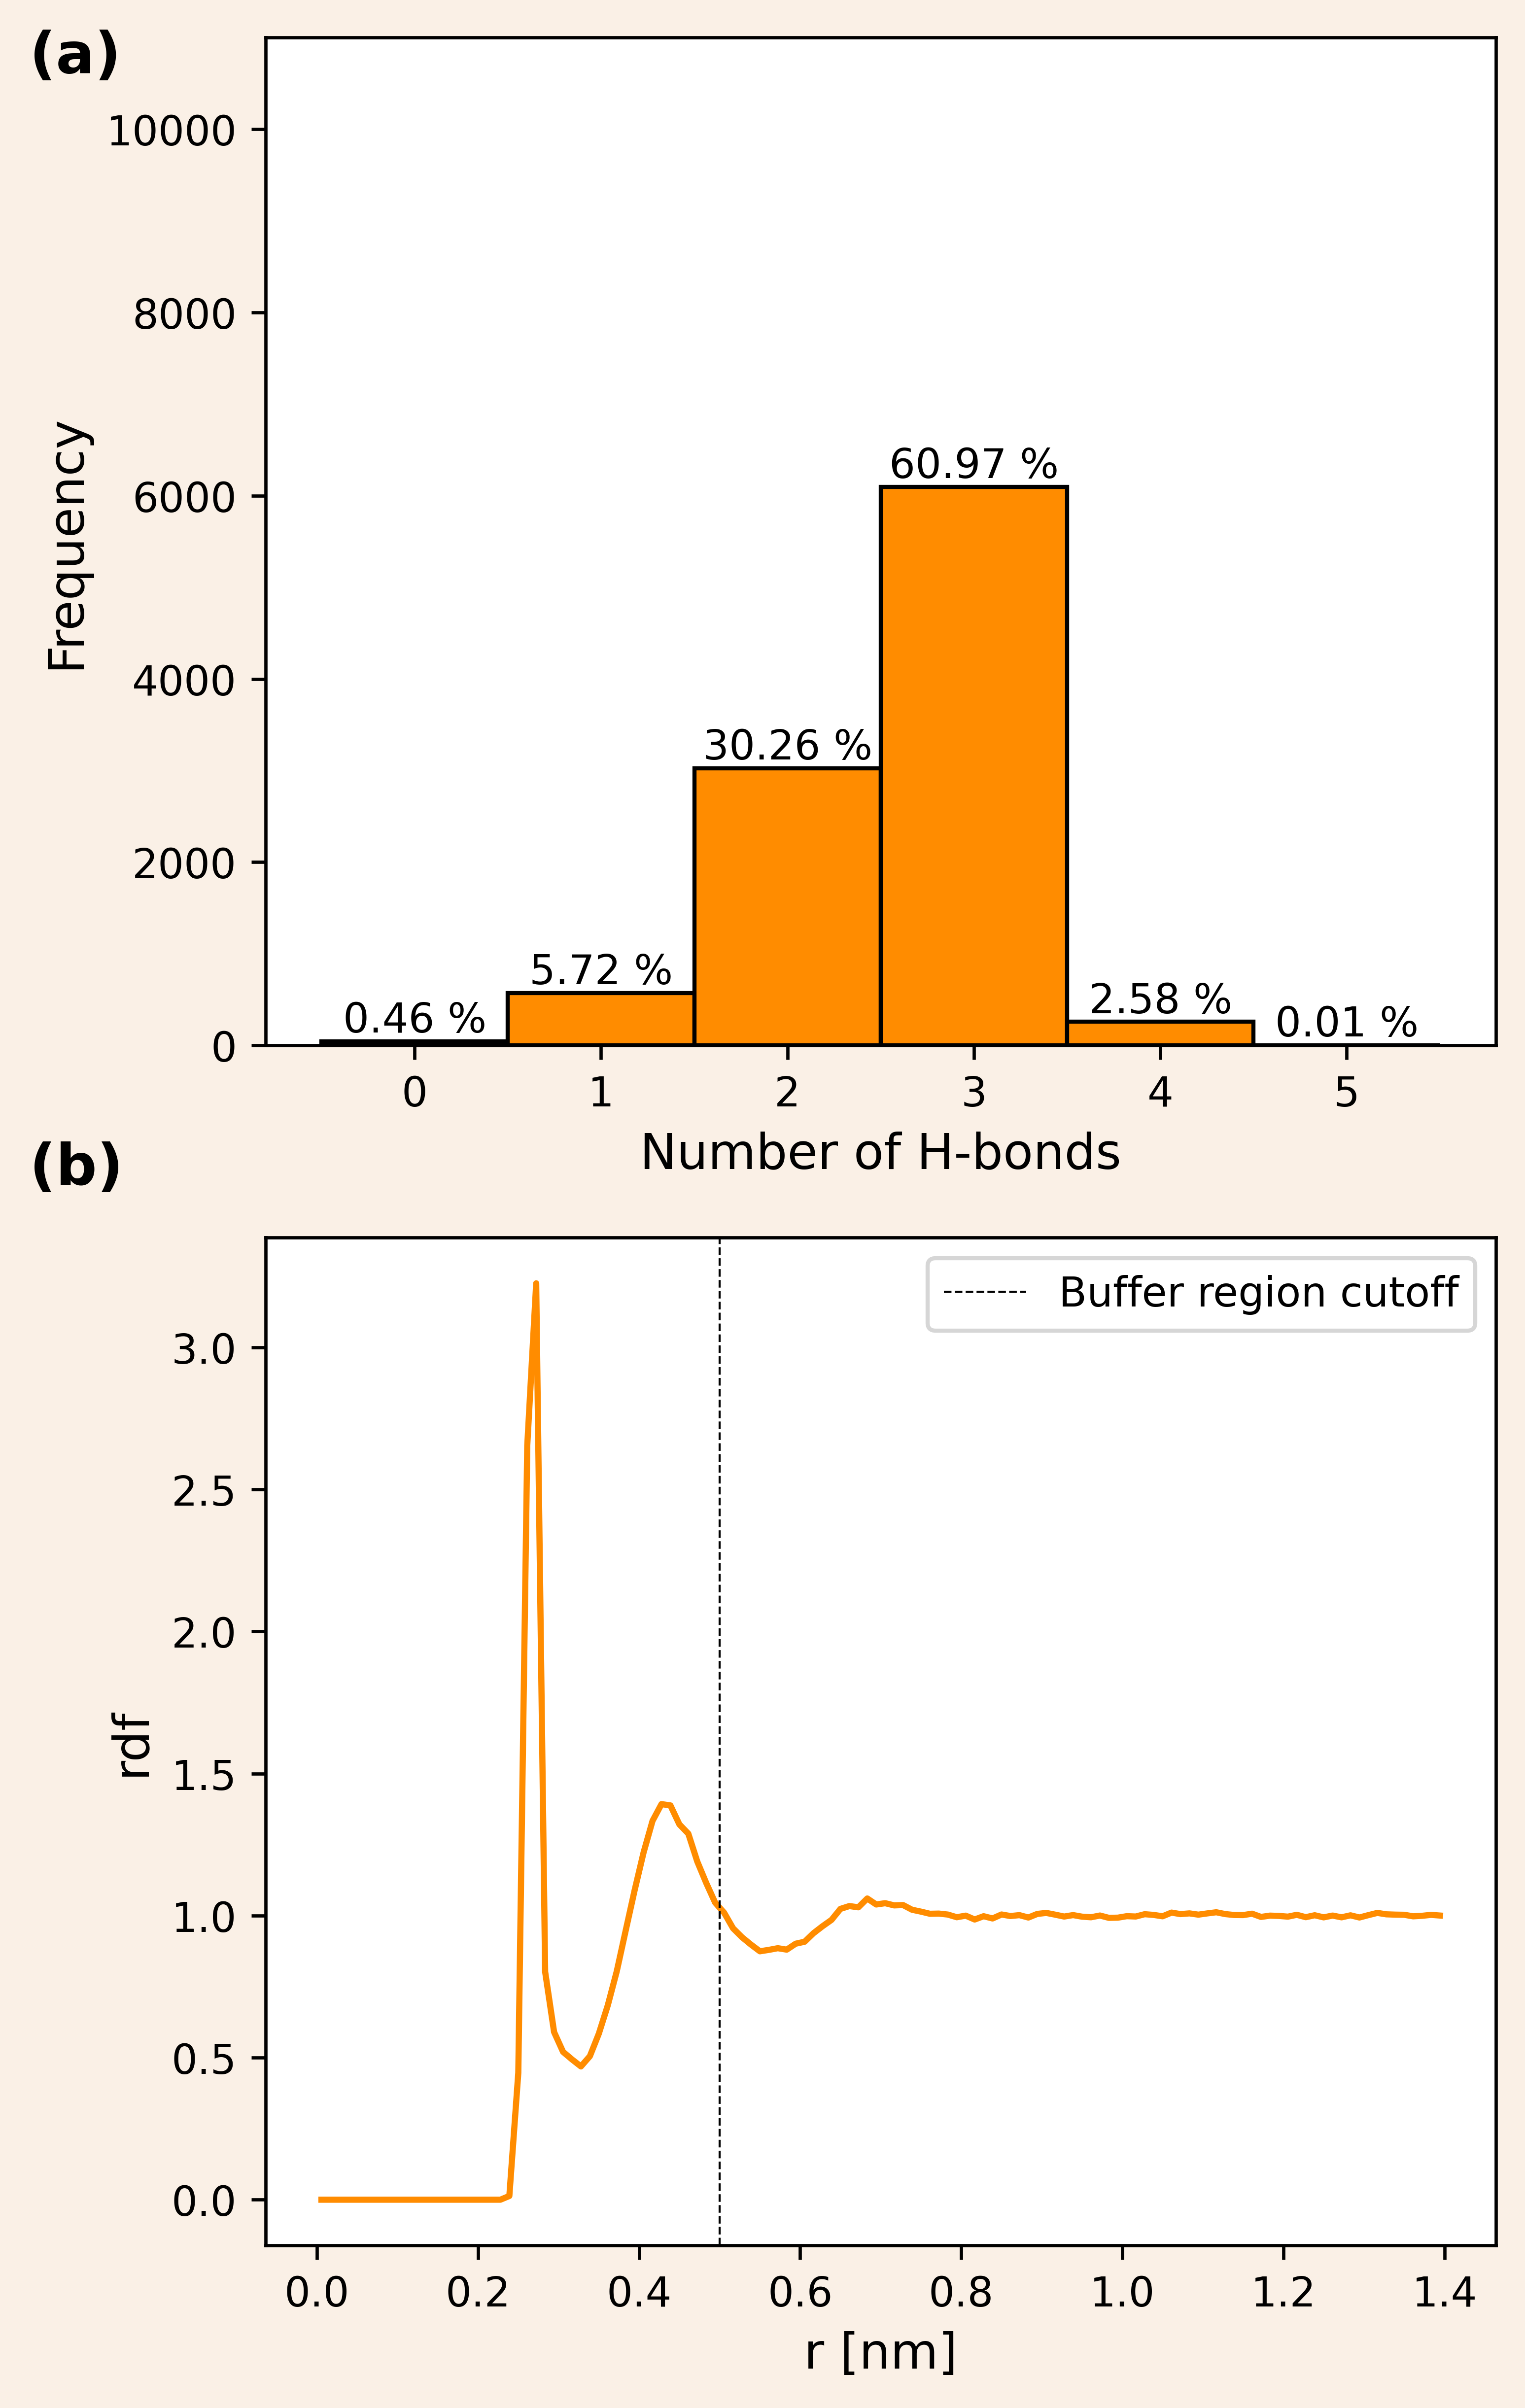
\includegraphics[scale=.66]{../09_tutorial_06/figures/BuRNN_ana.png}
\caption{\textbf{BuRNN simulation analysis. (a)} The number of hydrogen bonds formed between methanol and water for each snapshot of the trajectory. \textbf{(b)} Radial distribution function between the methanol's oxygen and all the oxygen atoms of the water molecules. The results are based on a 2 ns BuRNN simulation of the methanol in water.}
\label{BuRNN_ana}
\end{figure}



\subsubsection{Advanced options}
\paragraph{Charge model}
For running BuRNN simulations with dynamic QM charges, charges first need to be calculated with the QM method of choice and included in the training dataset. A separate NN has to be trained for the charges. SchNet was therefore adapted and the version can be found in \href{https://github.com/juliawestermayr/schnetpack}{this repository}.
In the \texttt{charge.qmm} file the \texttt{NNCHARGE} block has to be added. 

\begin{lstlisting}[breaklines=true, breakatwhitespace=false]
NNCHARGE
/path/to/best/charge_model
# NUMSTP
       1
END
\end{lstlisting}

This block contains the path to the NN charge model and how often (every \texttt{NUMSTP} steps) the charges should be updated.

Including a charge model was e.g. relevant for the hexa-aqua iron, the model system of the original BuRNN paper \cite{Lier2022BuRNN}. Where a considerable amount of charge transfer between the inner and buffer regions was observed, which needed to be reflected in their interactions with the outer region.

%\paragraph{Adaptive sampling}



\section{Author Contributions}
%%%%%%%%%%%%%%%%
% This section mustt describe the actual contributions of
% author. Since this is an electronic-only journal, there is
% no length limit when you describe the authors' contributions,
% so we recommend describing what they actually did rather than
% simply categorizing them in a small number of
% predefined roles as might be done in other journals.
%
% See the policies ``Policies on Authorship'' section of https://livecoms.github.io
% for more information on deciding on authorship and author order.
%%%%%%%%%%%%%%%%

%(Explain the contributions of the different authors here)
JG and NH prepared Tutorial 1, BL, C\"O, AdR and CO prepared Tutorials 2 and 3. OGC prepared Tutorial 4. BB prepared Tutorial 5. BL, RC, and PP prepared Tutorial 6. MBMS tested the tutorials. All authors contributed to manuscript writing.

% We suggest you preserve this comment:
%For a more detailed description of author contributions,
%see the GitHub issue tracking and changelog at \githubrepository.

\section{Other Contributions}

%%%%%%%%%%%%%%%
% You should include all people who have filed issues that were
% accepted into the paper, or that upon discussion altered what was in the paper.
% Multiple significant contributions might mean that the contributor
% should be moved to authorship at the discretion of the a
%
% See the policies ``Policies on Authorship'' section of https://livecoms.github.io for
% more information on deciding on authorship and author order.
%%%%%%%%%%%%%%%
This work has profited from the experiences of various members of the research groups of  WFvG, NH and CO using the methods explained in this tutorial.

%\textcolor{red}{(Explain the contributions of any non-author contributors here)}
% We suggest you preserve this comment:
%\textcolor{red}{For a more detailed description of contributions from the community and %others, see the GitHub issue tracking and changelog at \githubrepository.}

\section{Potentially Conflicting Interests}
%%%%%%%
%Declare any potentially competing interests, financial or otherwise
%%%%%%%
%Declare any potentially conflicting interests here, whether or not they pose an actual conflict in your view.
WFvG, CO and NH and their research groups are developers of the GROMOS simulation package.

\section{Funding Information}
%%%%%%%
% Authors should acknowledge funding sources here. Reference specific grants.
%%%%%%%
NH acknowledges funding by the Deutsche Forschungsgemeinschaft (DFG, German Research Foundation) under Germany’s Excellence Strategy – EXC 2075 – 390740016.
CO acknowledges the Austrian Federal Ministry for Digital and Economic Affairs, The National Foundation for Research, Technology and Development and the Christian Doppler Research Association for funding.

\section*{Author Information}
\makeorcid

\bibliography{livecoms-sample}

%%%%%%%%%%%%%%%%%%%%%%%%%%%%%%%%%%%%%%%%%%%%%%%%%%%%%%%%%%%%
%%% APPENDICES
%%%%%%%%%%%%%%%%%%%%%%%%%%%%%%%%%%%%%%%%%%%%%%%%%%%%%%%%%%%%

%\appendix


\end{document}
